%%	SECCION documentclass																									 %%	
%%---------------------------------------------------------------------------%%
\documentclass[a4paper]{report}

%%---------------------------------------------------------------------------%%
%%	SECCION usepackage																											 %%	
%%---------------------------------------------------------------------------%%
\usepackage{amsmath, amsthm}
\usepackage[spanish,activeacute]{babel}
\usepackage{caratula}
\usepackage{a4wide}
\usepackage{hyperref}
\usepackage{fancyhdr}
% \usepackage{moreverb}
\usepackage{graphicx} % Para el logo magico!
\usepackage{capt-of}
\usepackage{afterpage}
\usepackage{float}
\usepackage{amssymb}
\usepackage{amsmath}
\usepackage[latin1]{inputenc}
\usepackage{subfigure}
\usepackage[dvipsnames,usenames]{color}
\usepackage{amsfonts}
\usepackage{pdflscape}
\usepackage{booktabs}
\usepackage{colortbl}
\usepackage{tabularx}
\usepackage{dis}
%%---------------------------------------------------------------------------%%
%%	SECCION opciones																												 %%	
%%---------------------------------------------------------------------------%%
\parskip    = 11 pt
\headheight	= 13.1pt
\pagestyle	{fancy}
\definecolor{orange}{rgb}{1,0.5,0}

\addtolength{\headwidth}{1.0in}

\addtolength{\oddsidemargin}{-0.5in}
\addtolength{\textwidth}{1.0in}
\addtolength{\topmargin}{-0.5in}
\addtolength{\textheight}{0.7in}

%%---------------------------------------------------------------------------%%
%%	SECCION document	 %%	
%%---------------------------------------------------------------------------%%
\begin{document}
\renewcommand{\chaptername}{Parte }

%%---- Caratula -------------------------------------------------------------%%
\materia{Ingenier�a de Software I (2do cuatrimestre de 2008)}
\titulo{Trabajo Pr�ctico 1}

\integrante{Gonzalez, Emiliano}{426/06}{xjesse\_jamesx@hotmail.com}
\integrante{Gonzalez, Sergio}{481/06}{seges.ar@gmail.com}
\integrante{Mart'inez, Federico}{17/06}{federicoemartinez@gmail.com}
\integrante{Sainz-Tr�paga, Gonzalo}{454/06}{gonzalo@sainztrapaga.com.ar}
\grupo{Grupo 5}
\resumen{
Se presenta en este trabajo una especificaci�n completa de la soluci�n propuesta para el proyecto de software de
administraci�n de pizzer�a. En el mismo se presenta un panorama general as� como un an�lisis detallado del problema, 
y nuestra propuesta para su resoluci�n. En primer lugar se plantea una descripci�n general de la soluci�n, y a
continuaci�n se detallan algunos aspectos importantes haciendo uso de herramientas desarrolladas en clase como
diagramas de actividad, m�quinas de estado finito y otras.
}
\newcommand{\noig}{$<>$}
\newcommand{\negrita}[1]{{\bf #1}}
\newcounter{restriccion}
\setcounter{restriccion}{1}
\newcommand{\flecha}{\textcolor{Blue}{$\rightarrow$} }
\newcommand{\restr}[3]{
%\begin{tabularx}{14cm}{X}
\negrita{\therestriccion . #1:} \\
\negrita{Context #2} \\
\negrita{Inv:} \textsl{#3} \\
%\end{tabularx}
\stepcounter{restriccion}
}

% ----- Token list para las instrucciones ------------------------------------
\newtoks\oplist\oplist={}
% ----- Comando para que el usuario agregue operaciones del CU

\newcounter{PasoCu}
\setcounter{PasoCu}{1}

\newcommand{\op}[2]
{
\oplist=\expandafter{\the\oplist #1 & #2 \\ \hline}
\stepcounter{PasoCu}
}

\newcounter{casoUso}
\setcounter{casoUso}{1}

\definecolor{light-gray}{gray}{0.9}
\newcommand{\cu}[6]{ 
{\setlength{\arrayrulewidth}{1mm}

\begin{tabularx}{16cm}{|X|X|}
\hline
\multicolumn{2}{|>{\columncolor{Black}}l|}{\textcolor{White}{\negrita{Caso de Uso: #1}}} \\
\hline
\multicolumn{2}{|>{\columncolor{Black}}l|}{\textcolor{White}{\negrita{N�mero \thecasoUso}}} \\
\hline
\multicolumn{2}{|>{\columncolor{light-gray}}l|}{\negrita{Actores intervinientes: #2}} \\
\hline
\multicolumn{2}{|>{\columncolor{light-gray}}l|}{\negrita{Requerimientos relacionados: #3}} \\
\hline
\multicolumn{2}{|>{\columncolor{light-gray}}l|}{\negrita{Precondici�n: #4}} \\
\hline
\multicolumn{2}{|>{\columncolor{light-gray}}l|}{\negrita{Poscondici�n: #5}} \\
\hline
\multicolumn{1}{|>{\columncolor{light-gray}}X|}{\negrita{Descripcion:}} &
\multicolumn{1}{>{\columncolor{light-gray}}X|}{\negrita{#6}} \\
\hline
\multicolumn{1}{|>{\columncolor{light-gray}}X|}{\negrita{Curso normal}} &
\multicolumn{1}{>{\columncolor{light-gray}}X|}{\negrita{Curso alternativo}}\\
\hline
\the\oplist
\end{tabularx}
\stepcounter{casoUso}
}
\newtoks\oplist\oplist={}
}

\newcounter{req}
\setcounter{req}{1}


\newcommand{\desreq}[5]{
{\setlength{\arrayrulewidth}{1mm}
\begin{tabular}{|| c | p ||}
\multicolumn{1}{|>{\columncolor{Black}}c|}{\textcolor{White}{\negrita{Requerimiento:}}} &
\multicolumn{1}{|>{\columncolor{Black}}l|}{\textcolor{White}{#1}}\\
\hline
\multicolumn{1}{|>{\columncolor{light-gray}}c|}{\negrita{Numero:}} &
\multicolumn{1}{|l|}{\thereq}\\
\hline
\multicolumn{1}{|>{\columncolor{light-gray}}c|}{\negrita{Tipo:}} &
\multicolumn{1}{|l|}{#2}\\
\hline
\multicolumn{1}{|>{\columncolor{light-gray}}c|}{\negrita{Importancia:}} &
\multicolumn{1}{|l|}{#3}\\
\hline
\multicolumn{1}{|>{\columncolor{light-gray}}c|}{\negrita{Descripci�n:}} &
\multicolumn{1}{|p{13cm}|}{#4}\\
\hline
\multicolumn{1}{|>{\columncolor{light-gray}}c|}{\negrita{Motivo:}} &
\multicolumn{1}{|p{13cm}|}{#5}\\\hline
\end{tabular}
\stepcounter{req}
}
}

% TOC, usa estilos locos
\maketitle
\pagestyle{empty}
{
\fancypagestyle{plain}
    {
    \fancyhead{}
    \fancyfoot{}
    \renewcommand{\headrulewidth}{0.0pt}
    } % clear header and footer of plain page because of ToC
\tableofcontents
}

\newpage
% arreglos los estilos para el resto del documento, y
% reseteo los numeros de pagina para que queden bien
\pagenumbering{arabic}
\fancypagestyle{plain} {
    \fancyhead[LO]{Gonzalez, Gonzalez, Mart�nez, Sainz-Tr�paga}
    \fancyhead[C]{}
    \fancyhead[RO]{P\'agina \thepage\ de \pageref{LastPage}}
    \fancyfoot{}
    \renewcommand{\headrulewidth}{0.4pt}
}
\pagestyle{plain}

\chapter{Introducci�n}
\section{Objetivo del documento}
%\textcolor{Blue}{Aqu� se espera una breve introducci�n con respecto a este informe.}

% FIXME: completar
% sirve para
% validar que el software haga lo que piden
% especificar el comoportamiento para permitir el testing
% servir de lineamiento general para todo el desarrollo posterior
% servir  de introduccion y descripci�n general al problema para quienes necesiten entenderlo
% servir de documento de base para la creaci�n de otros documentos m�s precisos

\section{Convenciones de notaci�n}
%FIXME: papelon
En este documento CU se entiende como Caso de Uso.
%\textcolor{Blue}{Describir aqu� cualquier convenci�n de notaci�n que se utilice en el presente documento, de manera de facilitar la lectura y comprensi�n del mismo por parte de los destinatarios. Notar que esta secci�n no se refiere a la sintaxis de las t�cnicas a utilizar, sino de definir las condiciones, siglas, simbolog�a o abreviaturas utilizadas espec�ficamente por los autores en el documento. 
%Por ej.}

%\textcolor{ForestGreen}{ 	CdC: En el presente documento figurar�n con la presente notaci�n los comentarios especiales a la c�tedra respecto del presente informe.}

\section{Destinatarios del documento}
El presente documento est� dirigido en primer lugar al due�o y los empleados de la pizzer�a, con el objetivo de que lo revean y examinen la din�mica de uso del sistema para validar que las funcionalidades propuestas son correctas. A su vez, estas personas son id�neas para sugerir mejoras o modificaciones a la operatoria propuesta, ya que son las que en el futuro deber�n interactuar fluidamente con el software.

En segunda instancia, tambi�n son destinatarios del documento aquellas personas que supervisar�n el desarrollo del software por parte del cliente que lo encarg�, en particular el �rea de Calidad de Software designado por �ste, que utilizar� este documento como referencia de comportamiento del software a los efectos de realizar pruebas de funcionamiento y desempe�o.

% Empleados de la pizzer�a (que lo van a usar)
% Due�o de la pizzer�a (que se va a beneficiar de un mejor conocimiento del negocio)
% QA ("clientes" simulados por el �rea de calidad de software, deben conocer el funcionamiento te�rico del sistema)
% Algo mas?

\section{Descripci�n del problema}

El problema a abordar es la introducci�n de mejoras en la administraci�n de una pizzer�a. En particular, se deber�n resolver algunos problemas que con el mecanismo actual de organizaci�n son recurrentes y representan una dificultad importante en el d�a a d�a del negocio. Por otro lado, el sistema deber� mejorar todo el proceso de gesti�n y manejo de pedidos, con el objeto de acrecentar su rendimiento mediante el mejor uso de los recursos tanto f�sicos como humanos. Finalmente, el sistema debe tener en cuenta el proyecto de expansi�n de la pizzer�a mediante la generaci�n de nuevas formas de pedido y cobro, as� como la incorporaci�n de un servicio de \textit{delivery}. Es de crucial importancia que el sistema utilice su capacidad de registro para realizar estad�sticas que permitan conocer el rendimiento y las limitaciones en la producci�n de la pizzer�a.

Contamos entonces cuatro objetivos principales:
\begin{itemize}
\item Resolver los problemas de operaci�n actuales (evitar que se pierdan pedidos, evitar tomar pedidos que no pueden ser satisfechos)
\item Mejorar la administraci�n de la pizzer�a (gesti�n del stock, planeamiento eficaz del uso de hornos y cocina, informatizaci�n de las comunicaciones entre los participantes del proceso)
\item Ampliar las formas de pedido y pago, permitiendo ingresar pedidos por tel�fono, Web o SMS
\item Realizar an�lisis estad�sticos en base a la informaci�n registrada
\end{itemize}

%\textcolor{Blue}{Breve descripci�n del problema al que se refiere el proyecto.}

%%%%%%%%%%%%%%%%%%%%
% crecimiento de la pizzeria
% automatizar pizzeria
% control de pedidos
% incorporar nuevas formas de venta
%%%%%%%%%%%%%%%%%%%%%

% Atacar problemas funcionales: pedidos no satisfacibles, pedidos que se pierden o se procesan en desorden
% Brindar mejoras al negocio:
%  - Mejor aprovechamiento de recursos (tanto de mano de obra como de hornos y de stock)
%  - Mejor conocimiento de la din�mica del negocio mediante indicadores estad�sticos
%  - Ampliaci�n de formas de pedido
% Estas mejoras deber�an permitir "agrandar" el negocio atendiendo a m�s clientes y con mayor calidad.

\section{Documentos relacionados}
El principal documento a tener en cuenta es \textit{Enunciado TP V1}, donde se detallan los requerimientos e intenciones de los clientes a los efectos del sistema. Como no se hicieron reuniones formales para discutir la funcionalidad del sistema, no se dispone de minutas de reuniones ni ninguna otra fuente primaria de informaci�n. La gran mayor�a de las cuestiones que conciernen a la funcionalidad del sistema fueron explicadas en clase o discutidas por correo electr�nico con los docentes de la materia.


%\textcolor{Blue}{Se deber�an enumerar aqu� los diferentes documentos relacionados con el presente y que pueden ser de inter�s para el lector de este informe.}
%
%\textcolor{ForestGreen}{CdC: No se espera aqu� que detallen bibliograf�a sino documentaci�n de inter�s directo con el proyecto. Por ej., aqu� podr�an estar mencionadas las minutas de reuniones de relevamiento.}

\section{Organizaci�n del informe}
El presente documento se organiza de la siguiente manera:
\begin{enumerate}
\item Introducci�n: se presentan  los objetivos del documento, as� como una breve descripci�n del problema a resolver y del alcance de este documento.
\item Descripci�n: se presenta una descripci�n general de la soluci�n, su alcance y perspectiva, al tiempo que se presentan las caracter�sticas de los usuarios, limitaciones, supuestos y dependencias que pudieran afectar al software a desarrollar.
\item Consideraciones globales de la soluci�n: se describe la soluci�n desde un punto de vista global. En este apartado se encuentran los requerimientos del sistema, los principales casos de uso, conceptos y contexto de funcionamiento del software.
\item Aspectos particulares de la soluci�n: se analizan los distintos aspectos de la soluci�n desde una �ptica mas especifica a cada componente de la soluci�n. En este inciso se detallan cuestiones tales como el el ingreso de pedidos, el ciclo de vida de un pedido y la administraci�n de los hornos, entre otros.
\item Ap�ndice I - Extensiones: se detallan posibles extensiones y mejoras al software descripto previamente, que si bien est�n por fuera de la soluci�n propuesta podr�an ser de inter�s para futuras revisiones del producto.
\item Ap�ndice II - Glosario: se describe la terminolog�a utilizada en todo el documento para referirse a agentes, componentes y otros t�rminos relevantes que aparecen en este documento.
\end{enumerate}

%\textcolor{Blue}{Breve descripci�n del documento, aclaraciones sobre c�mo se debe leer, etc, etc.}

\chapter{Descripci�n General}
Dado que uno de los aspectos principales del problema es la organizaci�n de los pedidos, es una parte fundamental del producto controlar el estado de los mismo, permitir su ingreso controlado, asi como brindar un seguimiento que permita conocer que pasa con los pedidos ingresados. Por otro lado se espera que el software sea capaz de interactuar con diversos tipos de clientes a fin de lograr variadas formas de ingreso de pedidos.

El sistema deber� ademas ser capaz de brindar estadisticas que permitan estudiar el funcionamiento del negocio, asi como tambi�n realizar un seguimiento de los productos vendidos a fin de lograr buenos precios.
%\textcolor{Blue}{Esta secci�n busca describir los factores generales que afectan al producto y sus requerimientos. No se detallan aqu� los requerimientos espec�ficos, pero provee un conocimiento b�sico general para dichos requerimientos.}

\section{Perspectiva del producto}
El producto es autocontenido en lo referente a la gestion de los pedidos, asi como tambi�n en el manejo del stock de productos e insumos. Sin embargo el software no se encarga de la facturaci�n, ya que la misma
%\textcolor{Blue}{Esta secci�n encuadra el producto en la perspectiva con otros productos relacionados. Si el producto es independiente y totalmente autocontenido, dicha situaci�n deber�a explicitarse aqu�.}

\section{Funciones principales del producto} 
%\textcolor{Blue}{Esta secci�n deber�a proveer un resumen de las funciones principales que el producto debe realizar. }

El sistema se encarga de monitorear el ciclo de vida de los pedidos que se realizan a la pizzer�a y el stock de las materias primas. Es responsable tambi�n de la optimizaci�n del uso del horno, la estimaci�n de lapsos de producci�n y entrega, y por �ltimo de conservar un registro de los eventos de inter�s con fines estad�sticos. 

En el caso de los pedidos realizados remotamente (v�a Web o SMS), el sistema se encarga tambi�n de su ingreso. Para los pedidos realizados de forma directa (ya sea a un mesero o llamando por tel�fono) existir� un inviduo responsable de su ingreso.

Desde el momento del ingreso de los pedidos, el sistema verifica su factibilidad en funci�n del stock de insumos. Una vez ingresados los pedidos, el sistema actualiza la informaci�n de stock inmediatamente (y at�micamente junto con la inserci�n del pedido). A continuaci�n se inserta el pedido en la cola de pedidos y se presenta a quien ingres� el pedido (usuario o encargado) una estimaci�n de la demora en la preparaci�n del pedido.

Dentro de la cocina, los maestros pizzero y empanadero tienen acceso al sistema en el cual pueden observar los pedidos que deben preparar e indicar su estado de preparaci�n (en espera, preparado, en el horno). Tras la preparaci�n, si el pedido debe ser entregado el sistema contin�a monitoreando su estado y la demora en la entrega, tras la cual se recibe una notificaci�n por parte del delivery. El sistema env�a los datos de los pedidos que deben ser facturados al sistema de facturaci�n mediante un archivo en un formato especificado que contiene informaci�n tal como la cantidad de items, su precio y la forma de pago.

En todo momento el encargado de pedidos puede reordenar la cola de pedidos, o cancelar alguno de ellos, as� como los usuarios pueden consultar el estado de los mismos (v�a Web). Un segundo encargado responsable de stock (que puede o no ser la misma persona f�sica que el encargado de pedidos) puede actualizar el stock de insumos.

El sistema no es responsable de la log�stica de la distribuci�n ni de la interacci�n directa con los clientes que no utilizan los medios Web o SMS. Tampoco existen operaciones automatizadas que afecten al negocio: todo lo que el sistema hace es coordinar a los actores que participan. El proceso de preparaci�n y cocci�n de los alimentos es totalmente manual, as� como lo es la reposici�n del stock y el armado de los pedidos para su posterior entrega.

\section{Caracter�sticas de los usuarios}
%\textcolor{Blue}{Esta secci�n deber�a describir las caracter�sticas generales de los usuarios para los que est� pensado el producto.} 

Dadas las caracter�sticas mencionadas anteriormente sobre el producto, resulta imprescindible que los usuarios que interact�an con el sistema tengan conocimiento de como utilizarlo.

Es el caso de los empleados del local, los mozos deben saber como utilizar las computadoras de mano que le ser�n dadas para ingresar nuevos pedidos al sistema. En el caso de los maestros dentro de la cocina (ya sea el maestro empanadero, o el maestro pizzero) es necesario que sepan como pedirle al sistema el pr�ximo pedido a preparar, y adem�s como realizar los diferentes cambios de estado por los que pasa un pedido (desde que se comienza a preparar, hasta que ya se tiene el pedido listo para entregar) utilizando la pantalla de tipo touchscreen. Por �ltimo, el encargado de pedidos, que es el encargado de ingresar todos los pedidos que no sean remotos, cancelarlos, administrar las asignaciones a los hornos, y con la posibilidad de realizar consultas estad�sticas, debe estar capacitado para poder desempe�arse sin tener inconvenientes. 

Si bien no se requieren empleados con conocimientos tecnicos, si se espera que estos sepan interactuar con el sistema de manera fluida. Por esta raz�n podria ser necesario un periodo de capacitaci�n para que los distintos actores aprendar como utilizar correctamente el sistema.

Con respecto a los clientes, aquellos que quieran realizar pedidos via WEB deber�n saber como desempe�arse en internet, es decir tener m�nimos conocimientos del uso de un navegador de internet y como ingresar a las distintas paginas. Los usuarios que quieran utilizar el servicio, haciendo un pedido mediante mensajes de tipo SMS deber�n saber como utilizar un tel�fono celular para enviar los mensajes, adem�s saber cual es el n�mero al cual deben enviarlos para que el sistema los reciba. Aquellos usuarios que utilicen el tel�fono, deber�n saber como realizar una llamada y cual es el n�mero telef�nico del local.

\section{Restricciones}
Dado que a nivel presupuestario no hay restricciones, en principio la soluci�n no cuenta con limitaciones a nivel hardware. Basicamente se espera que las terminales del local sean computadoras actuales.

Con respecto al lenguaje o plataforma de desarrollo, tampoco se presentaron restricciones. %Intentamos hacerlo en haskell pero al maestro no le gustaba el pattern matching, probamos con hq9+ pero no era turing completo y no nos alcanzo :D

%TODO: no me da la cara para seguir escribiendo

%\textcolor{Blue}{Esta secci�n deber�a proveer una descripci�n general de cualquier cuesti�n que limite las opciones del desarrollador (ej, regulaciones, limitaciones de hardware, requerimientos sobre lenguajes de alto nivel, etc.)}

\section{Supuestos y dependencias}
%TODO: aca tampoco
%\textcolor{Blue}{Esta secci�n deber�a enumerar cada uno de los factores que afectan los requerimientos declarados en el documento. Estos factores no son restricciones de dise�o del software, sino m�s bien representan cuestiones cuyo cambio puede afectar los requerimientos.}


\chapter{Consideraciones globales de la soluci�n}

El objetivo de esta secci�n es evaluar el problema en su totalidad y describir la soluci�n propuesta desde un punto de vista hol�stico. En la secci�n siguiente se detallar�n de forma m�s precisa varios aspectos t�cnicamente importantes de lo aqu� descripto. Sin embargo, optamos por realizar esta descripci�n de lo general a lo particular para ofrecer una mayor claridad en la explicaci�n sin resignar detalle en los puntos importantes.

\section{Contexto del sistema}

A continuaci�n presentamos el contexto y las interacciones que realiza el sistema con el mundo exterior mediante el diagrama de contexto de nuestra soluci�n.

El objetivo de este diagrama es modelar la interfaz del sistema con sus usuarios y con los dem�s agentes involucrados en su funcionamiento.
Las flechas est�n coloreadas del mismo color que los agentes responsables de controlar los eventos representados por esas flechas, para mayor claridad en la lectura del diagrama.

R�pidamente puede verse que los agentes que m�s trascendencia tienen son el encargado de pedidos y el cliente. Desde el punto de vista del sistema, estos dos agentes tienen una gran participaci�n. El encargado de pedidos se encarga de toda la coordinaci�n de la producci�n y de la priorizaci�n de pedidos antes de su entrada a la cocina. Los clientes, por su parte, en raz�n de que pueden autogestionarse ingresando pedidos a trav�s de la Web o de SMS, necesitan tambi�n una interfaz rica en funcionalidades.

Otros agentes de importancia son el Mozo, el Cajero, el Delivery  y los Maestros, que tambi�n tienen interacci�n directa con el sistema y participan activamente en toda la din�mica de la pizzer�a, incluyendo tambi�n muchas actividades que no pasan por el sistema pero que son esenciales para su funcionamiento.

Por �ltimo tenemos agentes que son de menor jerarqu�a por la cantidad de operaciones que realizan. Podemos contar entre estos al encargado de stock, al due�o y a los sistemas bancario y de facturaci�n, que tienen roles m�s tangenciales y solo interact�an con el sistema de forma m�s espor�dica.

En raz�n de estas observaciones, ser� razonable destinar un tiempo acorde a la importancia de cada agente a pulir las interfases que lo conciernen. Esto es particularmente cr�tico para el caso de los clientes, en que disponer de una buena interfaz amigable y pr�ctica en lugar de una mala puede ser la diferencia entre realizar o no una venta.

Por �ltmo cabe aclarar que este diagrama representa el modo de operaci�n normal. Existe un modo de operatoria de contingencia donde las interacciones se ven modificadas. Esta alternativa de contingencia se discute en la secci�n 4.10, donde se incluye un segundo diagrama de contexto representativo de ese escenario.

\begin{figure}[H]
\centering
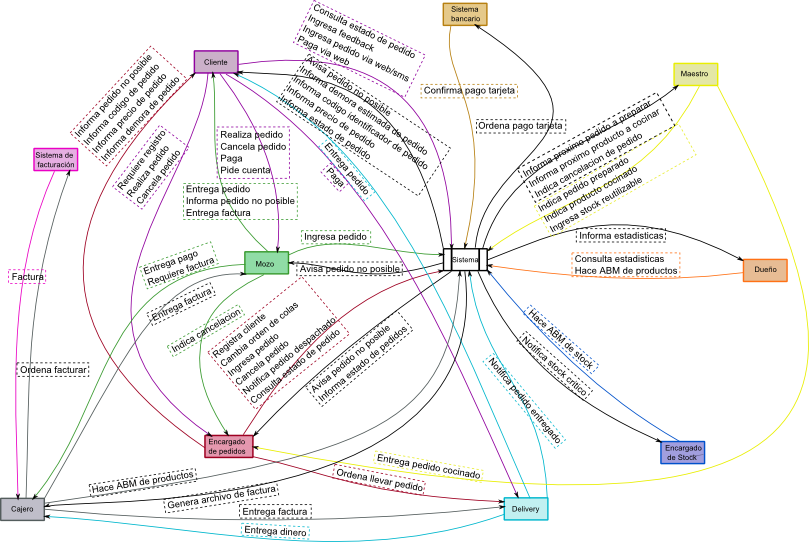
\includegraphics[angle=90,width=16cm]{./figuras/ContextoNormal.png}
\end{figure}

\section{Objetivos de la soluci�n y requerimientos del sistema}
A continuaci�n se presenta el diagrama de objetivos de la soluci�n, junto con un detalle de los requerimientos del sistema. 


\begin{figure}[H]
\centering
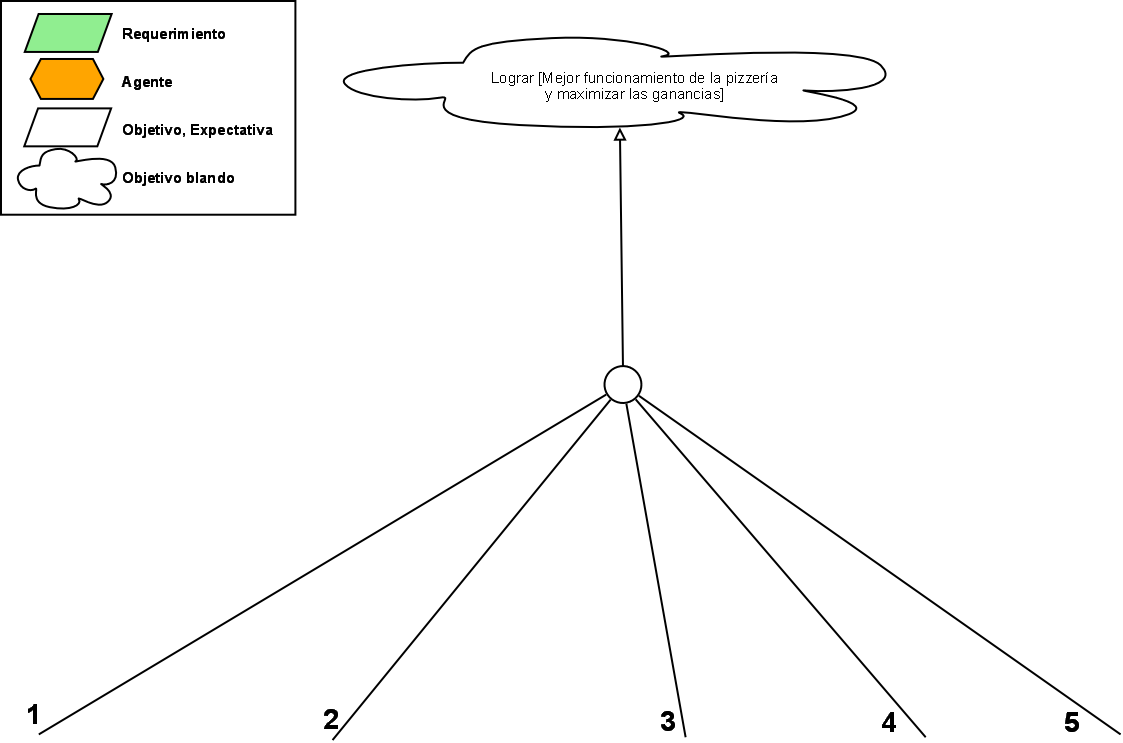
\includegraphics[height=13cm,angle=90]{./figuras/DiagramaObjetivos4.png}
\end{figure}

\begin{landscape}
\begin{figure}
\centering
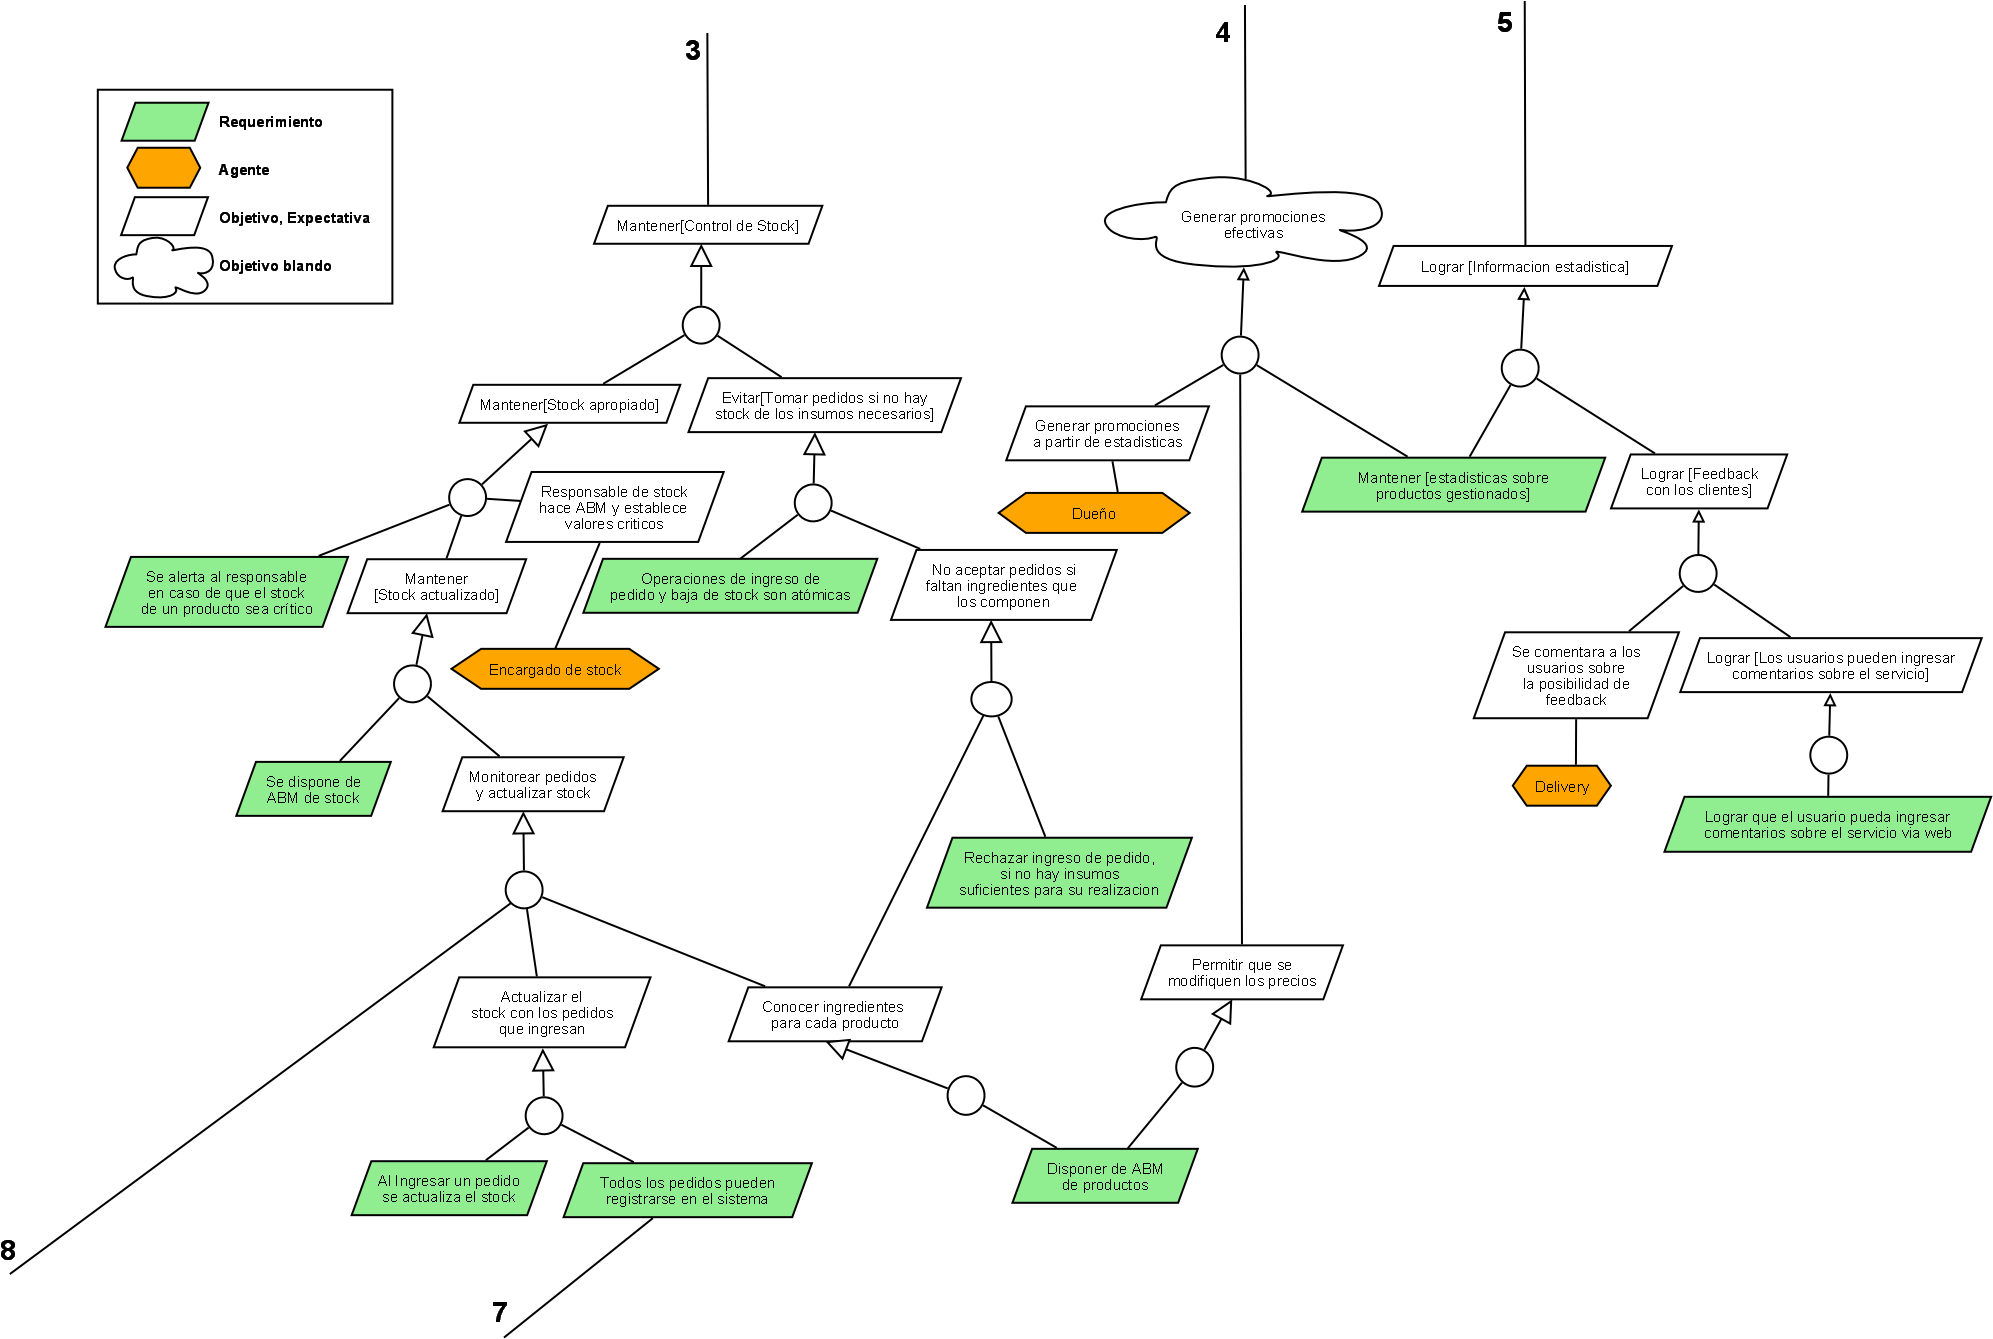
\includegraphics[height=16cm]{./figuras/DiagramaObjetivos3.png}
\end{figure}
\end{landscape}

% FIXME: hay que revisar todas las clasificaciones de esencial/importante y funciona/no funcional

\desreq{Se alerta al responsable en caso de que el stock de un producto sea cr�tico}
{Funcional}
{Esencial}
{Cuando el stock de un producto queda por debajo de un l�mite preestablecido, se debe generar un mensaje dirigido al responsable de stock a fin de notificar esta situaci�n.}
{Es una funcionalidad pedida expl�citamente, que ayuda a mantener un stock apropiado de los distintos productos y evitar as� la falta de insumos para realizar pedidos.}

\desreq{Se dispone de ABM de stock}
{Funcional}
{Importante}
{El sistema debe permitir que las altas, bajas y modificaciones de productos se registren en el sistema, para de esta manera controlar el stock de las materias primas y bebidas.}
{Mantener el stock de insumos actualizados, lo que contribuye a tener un control de stock apropiado.}

\desreq{Al ingresar pedido se actualiza el stock}
{Funcional}
{Importante}
{El sistema decrementar� el stock de materias primas o bebidas necesarias para un pedido al momento en que este ingresa al sistema.}
{Permite que el ingreso de pedidos modifique el stock consistentemente y de esta manera tener un stock actualizado.}

\desreq{Todos los pedidos pueden registrarse en el sistema}
{Funcional}
{Esencial}
{Los pedidos realizados pueden ingresarse al sistema y registrarse.}
{Este requerimiento ayuda controlar el stock de insumos y conocer el estado de los pedidos.}

\desreq{Operaciones de ingreso de pedido y baja de stock son at�micas}
{No funcional}
{Importante}
{El ingreso de un pedido y la disminuci�n del stock de sus materias primas son indisociables. Esto garantiza la consistencia del sistema de stock asegurando as� que los recursos necesarios para la realizaci�n de un pedido est�n efectivamente disponibles al momento de su ingreso.}
{Evitar tomar pedidos si no se dispone de los recursos para satisfacerlos.}

\desreq{Rechazar ingreso de pedido si no hay insumos suficientes para su realizaci�n}
{Funcional}
{Esencial}
{Si cuando se realiza un pedido no se dispone de los recursos necesarios para completarlo, el mismo no debe ingresar al sistema y se debe notificar a quien est� intentando realizar el pedido de dicha situaci�n}
{Evitar tomar pedidos si no se dispone de los recursos para satisfacerlos.}

\desreq{Disponer de ABM de productos}
{Funcional}
{Importante}
{Se debe proveer de una interfaz para registrar nuevos productos al men� (por ejemplo, nuevas variedades de pizza) as� como tambi�n modificar precios de productos ya registrados o sacarlos del men�.}
{Permitir modificaciones al men� y a la lista de precios.}

\desreq{Mantener estad�sticas sobre productos gestionados}
{Funcional}
{Esencial}
{El sistema debe ser capaz de retener la informaci�n sobre los productos que se gestionan para poder realizar estad�sticas sobre los pedidos, y de esta forma conocer m�s el funcionamiento de la pizzer�a.}
{Se pide de forma expl�cita tener informaci�n estad�stica sobre el funcionamiento de la pizzer�a, los pedidos, las cancelaciones, y productos m�s vendidos para hacer promociones.}

\desreq{Lograr que el usuario pueda ingresar comentarios sobre el servicio v�a web}
{Funcional}
{Deseable}
{Como aporte original proponemos que el usuario pueda ingresar comentarios sobre el servicio luego de recibir un pedido. El sistema debe ser capaz de registrar esos comentarios v�a Web.}
{Este requerimiento ayuda a generar informaci�n estadistica, con el objetivo de mejorar el servicio.}

\begin{landscape}
\begin{figure}
\centering
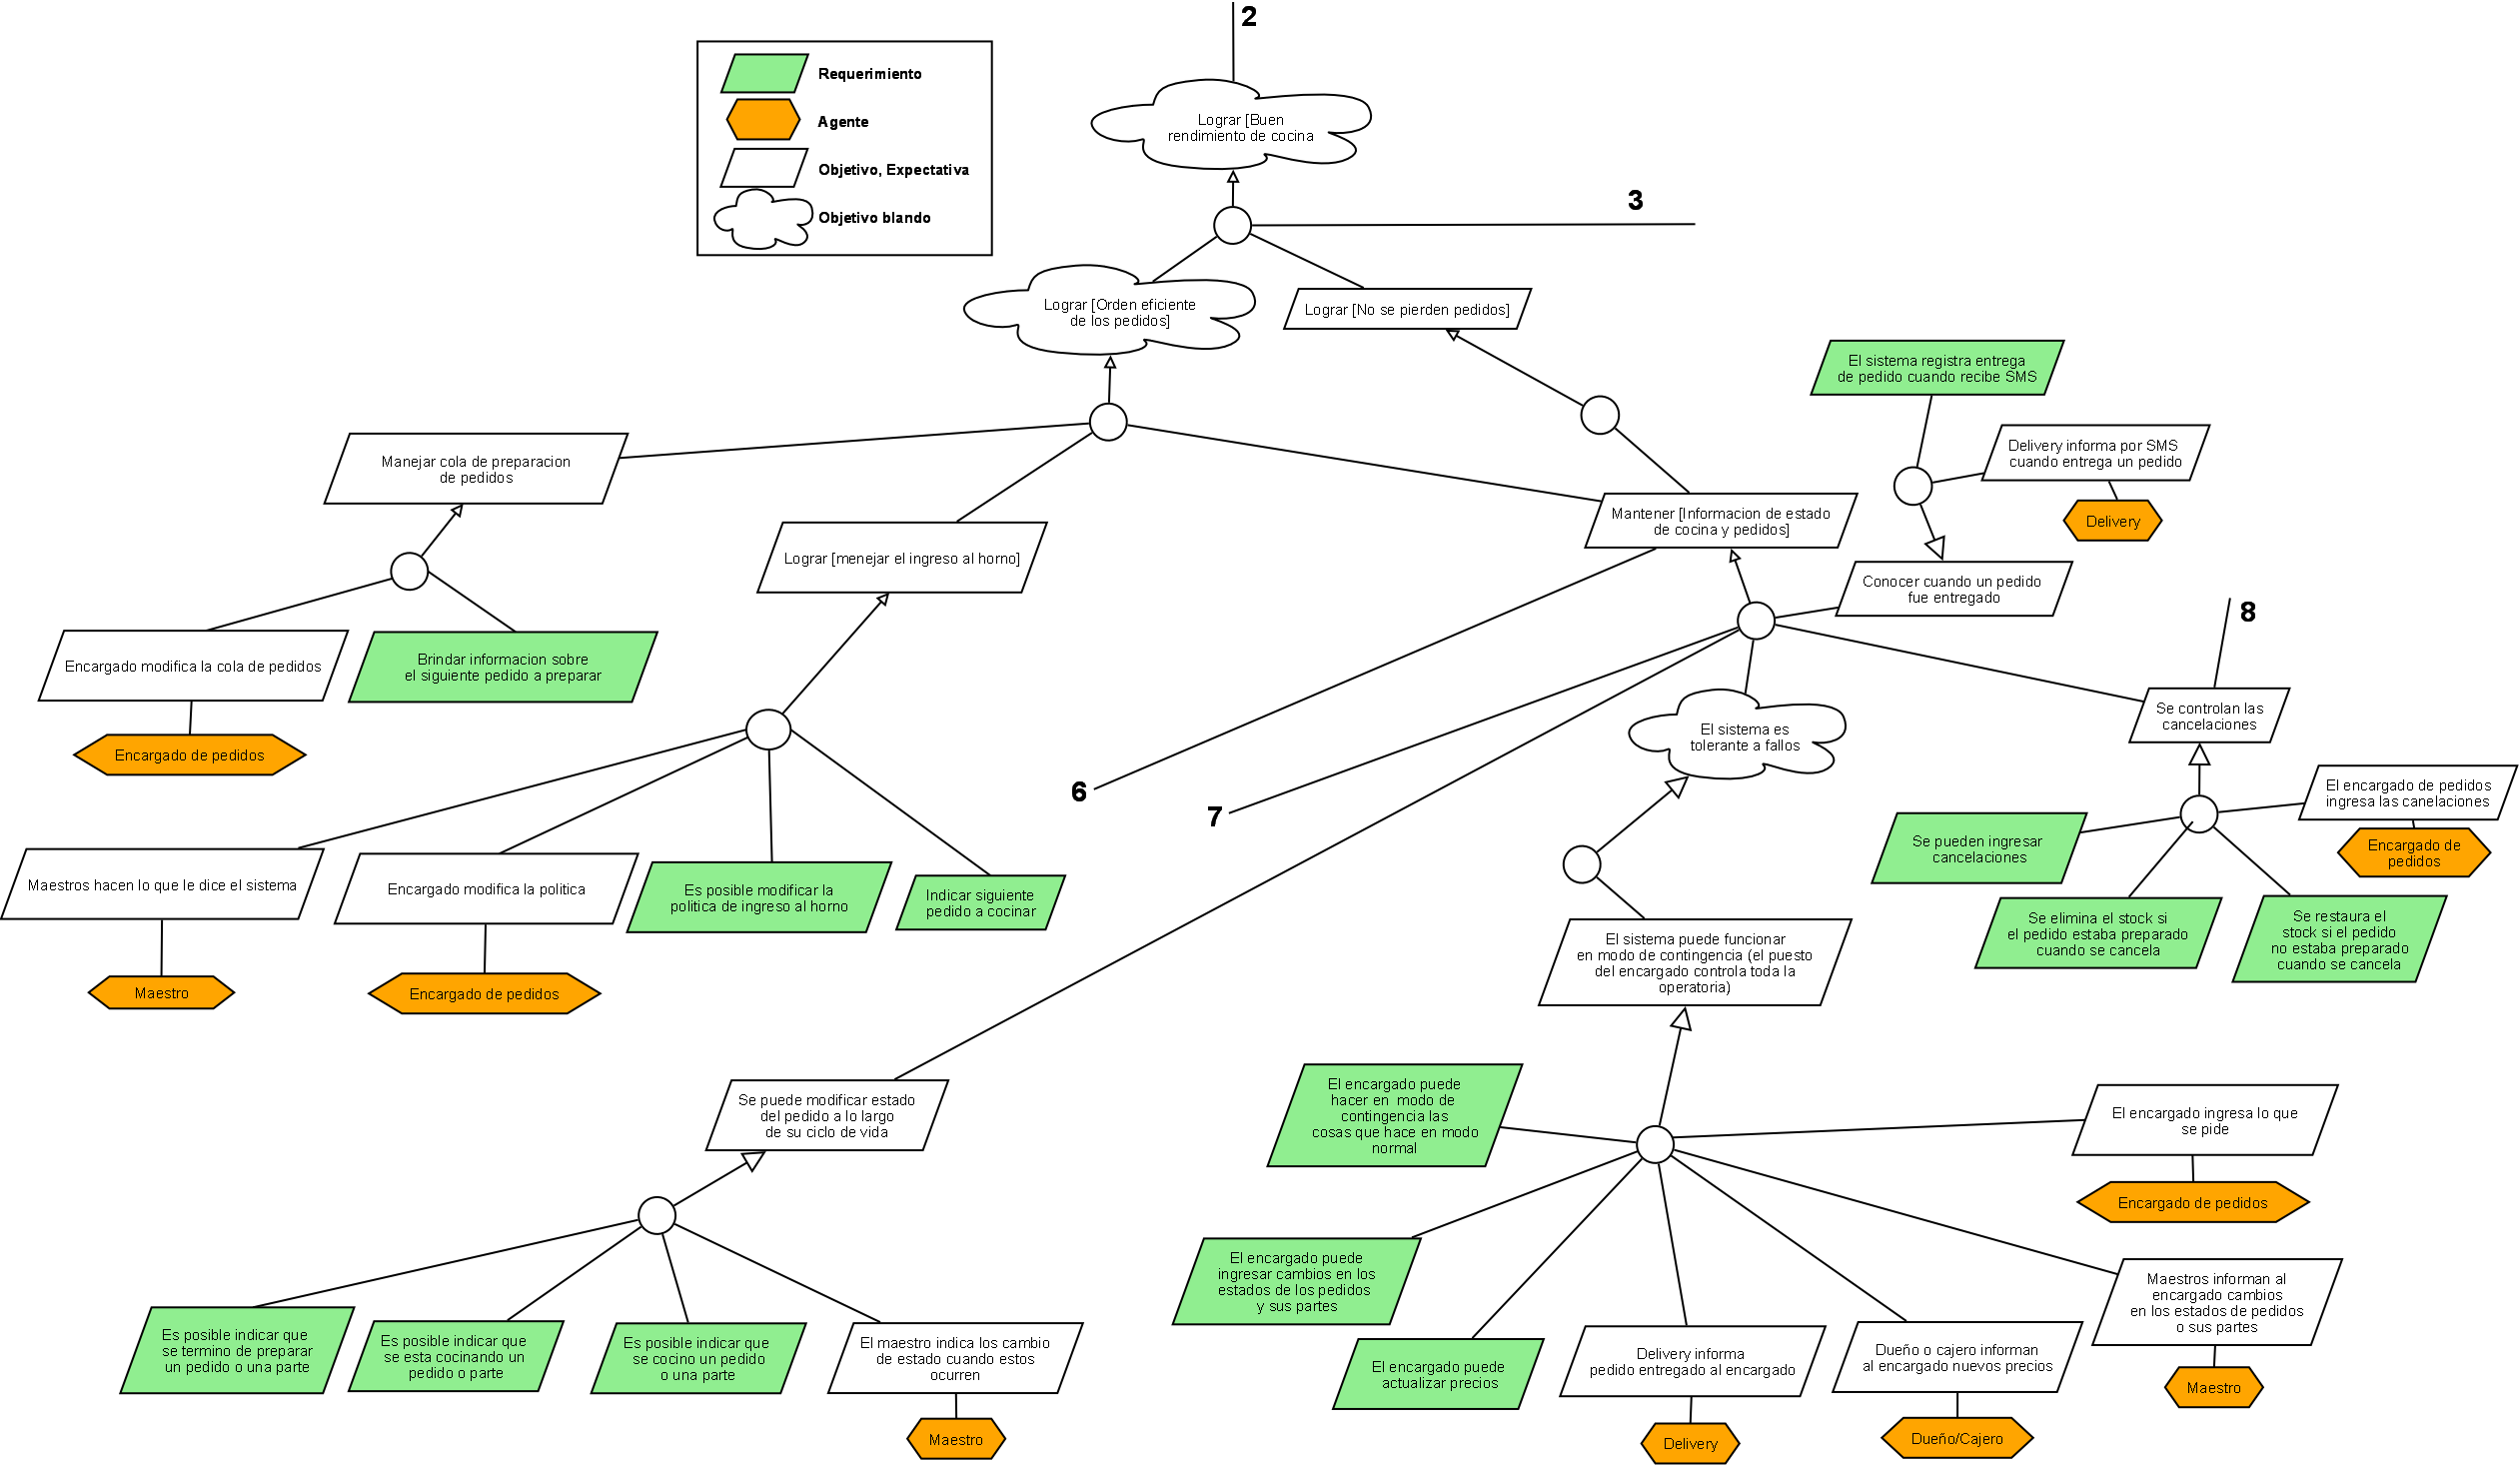
\includegraphics[height=17cm]{./figuras/DiagramaObjetivos2.png}
\end{figure}
\end{landscape}

\desreq{Es posible indicar que se termin� de preparar un pedido o una parte}
{Funcional}
{Importante}
{Cuando se prepara un pedido (o una parte de �l), debe ser posible indicar al sistema la tarea que se ha realizado.}
{Permite mantener actualizado el estado del pedido, adem�s de contribuir a la funcionalidad de poder cambiar el estado del mismo a lo largo de su ciclo de vida.}

\desreq{Es posible indicar que se est� cocinando un pedido o una parte}
{Funcional}
{Importante}
{Cuando un pedido est� preparado, el maestro puede comenzar a cocinar el pedido completo o una parte de �l. En cualquiera de los dos casos se debe poder indicar al sistema que ese pedido o parte del mismo se comenz� a cocinar.}
{Ayuda a poder modificar el estado del pedido a lo largo de su ciclo de vida, adem�s de controlar el estado del mismo.}

\desreq{Es posible indicar que se cocin� un pedido o una parte}
{Funcional}
{Importante}
{Cuando el maestro termina de cocinar un pedido o una parte de �l, debe poder indicarlo al sistema.}
{Ayuda a poder modificar el estado del pedido a lo largo de su ciclo de vida y controlar el estado del mismo.}

\desreq{Brindar informaci�n sobre el siguiente pedido a preparar}
{Funcional}
{Importante}
{El sistema administra los pedidos que se encuentran esperando a ser preparados en una cola de preparaci�n de los mismos, de esta se forma indica que pedido es el que sigue y por ende, cual es el que se tiene que preparar.}
{Permite manejar la cola de pedidos que se encuentran esperando para ser preparados, y adem�s contribuye a tener un orden eficiente de los pedidos que deben ingresar a la cocina.}

\desreq{Es posible modificar la pol�tica de ingreso al horno}
{Funcional}
{Importante}
{El encargado de pedidos puede realizar una modificaci�n de la pol�tica que administra los pedidos que requieren ingresar al horno para ser cocinados.}
{Permite tener un mejor control de los pedidos que ingresar�n al horno, y contribuir as� a tener un buen rendimiento en la cocina.}

\desreq{Indicar siguiente pedido a cocinar}
{Funcional}
{Importante}
{El sistema le indica al maestro que es lo que se debe cocinar a continuaci�n cuando �ste tenga la oportunidad de hacerlo.}
{Este requerimiento contribuye al manejo del ingreso de los pedidos al horno, con el fin de tener un buen rendimiento de la cocina.}

\desreq{El encargado puede hacer en contingencia las cosas que hace en modo normal}
{Funcional}
{Importante}
{Cuando el sistema se encuentra en modo de contingencia, el encargado de pedidos va a poder continuar haciendo las funciones que tiene asignadas en modo normal.}
{Este requerimiento aporta al funcionamiento del sistema en modo de contingencia permitiendo que el mismo sea tolerante a fallas.}

\desreq{El encargado puede ingresar cambios en los estados de los pedidos y sus partes}
{Funcional}
{Importante}
{Cuando el sistema se encuentra en modo de contingencia, es el encargado de pedidos el responsable de realizar las funcionalidades no disponibles para los actores que normalmente son responsables. En este caso, el encargado de pedidos deber� poder realizar los cambios de estado de los diferentes pedidos y sus respectivas partes. }
{Este requerimiento ayuda a que no se pierda la funcionalidad del sistema en modo de contingencia, ayudando a que el mismo sea tolerante a fallas.}

\desreq{El encargado puede actualizar precios}
{Funcional}
{Importante}
{El encargado puede realizar cambios en los precios de los productos cuando el sistema se encuentra en modo de contingencia.}
{Ayuda a que la funcionalidad del sistema no se pierda en modo de contingencia, lo que contribuye a que �ste sea tolerante a fallas.}

\desreq{Se pueden ingresar cancelaciones}
{Funcional}
{Importante}
{El sistema debe permitir que un pedido pueda ser cancelado, sin importar el estado en el que se encuentre. La excepci�n es el estado finalizado, que caracteriza al mismo cuando el mozo llev� el pedido a la mesa, el cliente retir� el pedido del mostrador o cuando el delivery logr� entregar el pedido.}
{Este requerimiento contribuye al control de las cancelaciones, que permite mantener informaci�n sobre el estado de los pedidos.}

\desreq{Se elimina el stock si el pedido estaba preparado cuando se cancela}
{Funcional}
{Importante}
{Los productos ya preparados o cocinados de un pedido no se pueden reutilizar, por lo que deben ser descartados. Este requerimiento est� relacionado con que este descarte sea automatico, es decir que no se tengan que ingresar las bajas de stock correspondientes de forma manual.}
{Provee un m�todo para controlar las cancelaciones de pedidos y seguir el stock con facilidad. Como el descarte es autom�tico, ayuda tambi�n a llevar el estado del stock.}

\desreq{Se restaura el stock si el pedido no estaba preparado cuando se cancela}
{Funcional}
{Importante}
{Si se cancela un pedido antes de prepararlo, las materias primas que no se usaron deben volver al stock a fin de que puedan ser usadas para preparar un nuevo pedido. Dicha funcionalidad es autom�tica.}
{Permite controlar las cancelaciones, mejorar la eficiencia de la cocina, y contribuye a llevar el estado del stock.}

\desreq{El sistema registra entrega de pedido cuando recibe SMS}
{Funcional}
{Importante}
{Cuando el delivery manda un mensaje SMS al sistema con el pedido que se entreg�, �ste registra al pedido como finalizado.}
{Este requerimiento contribuye a conocer cuando un pedido fue entregado, para mantener informaci�n de estado de los pedidos.}

\begin{landscape}
\begin{figure}
\centering
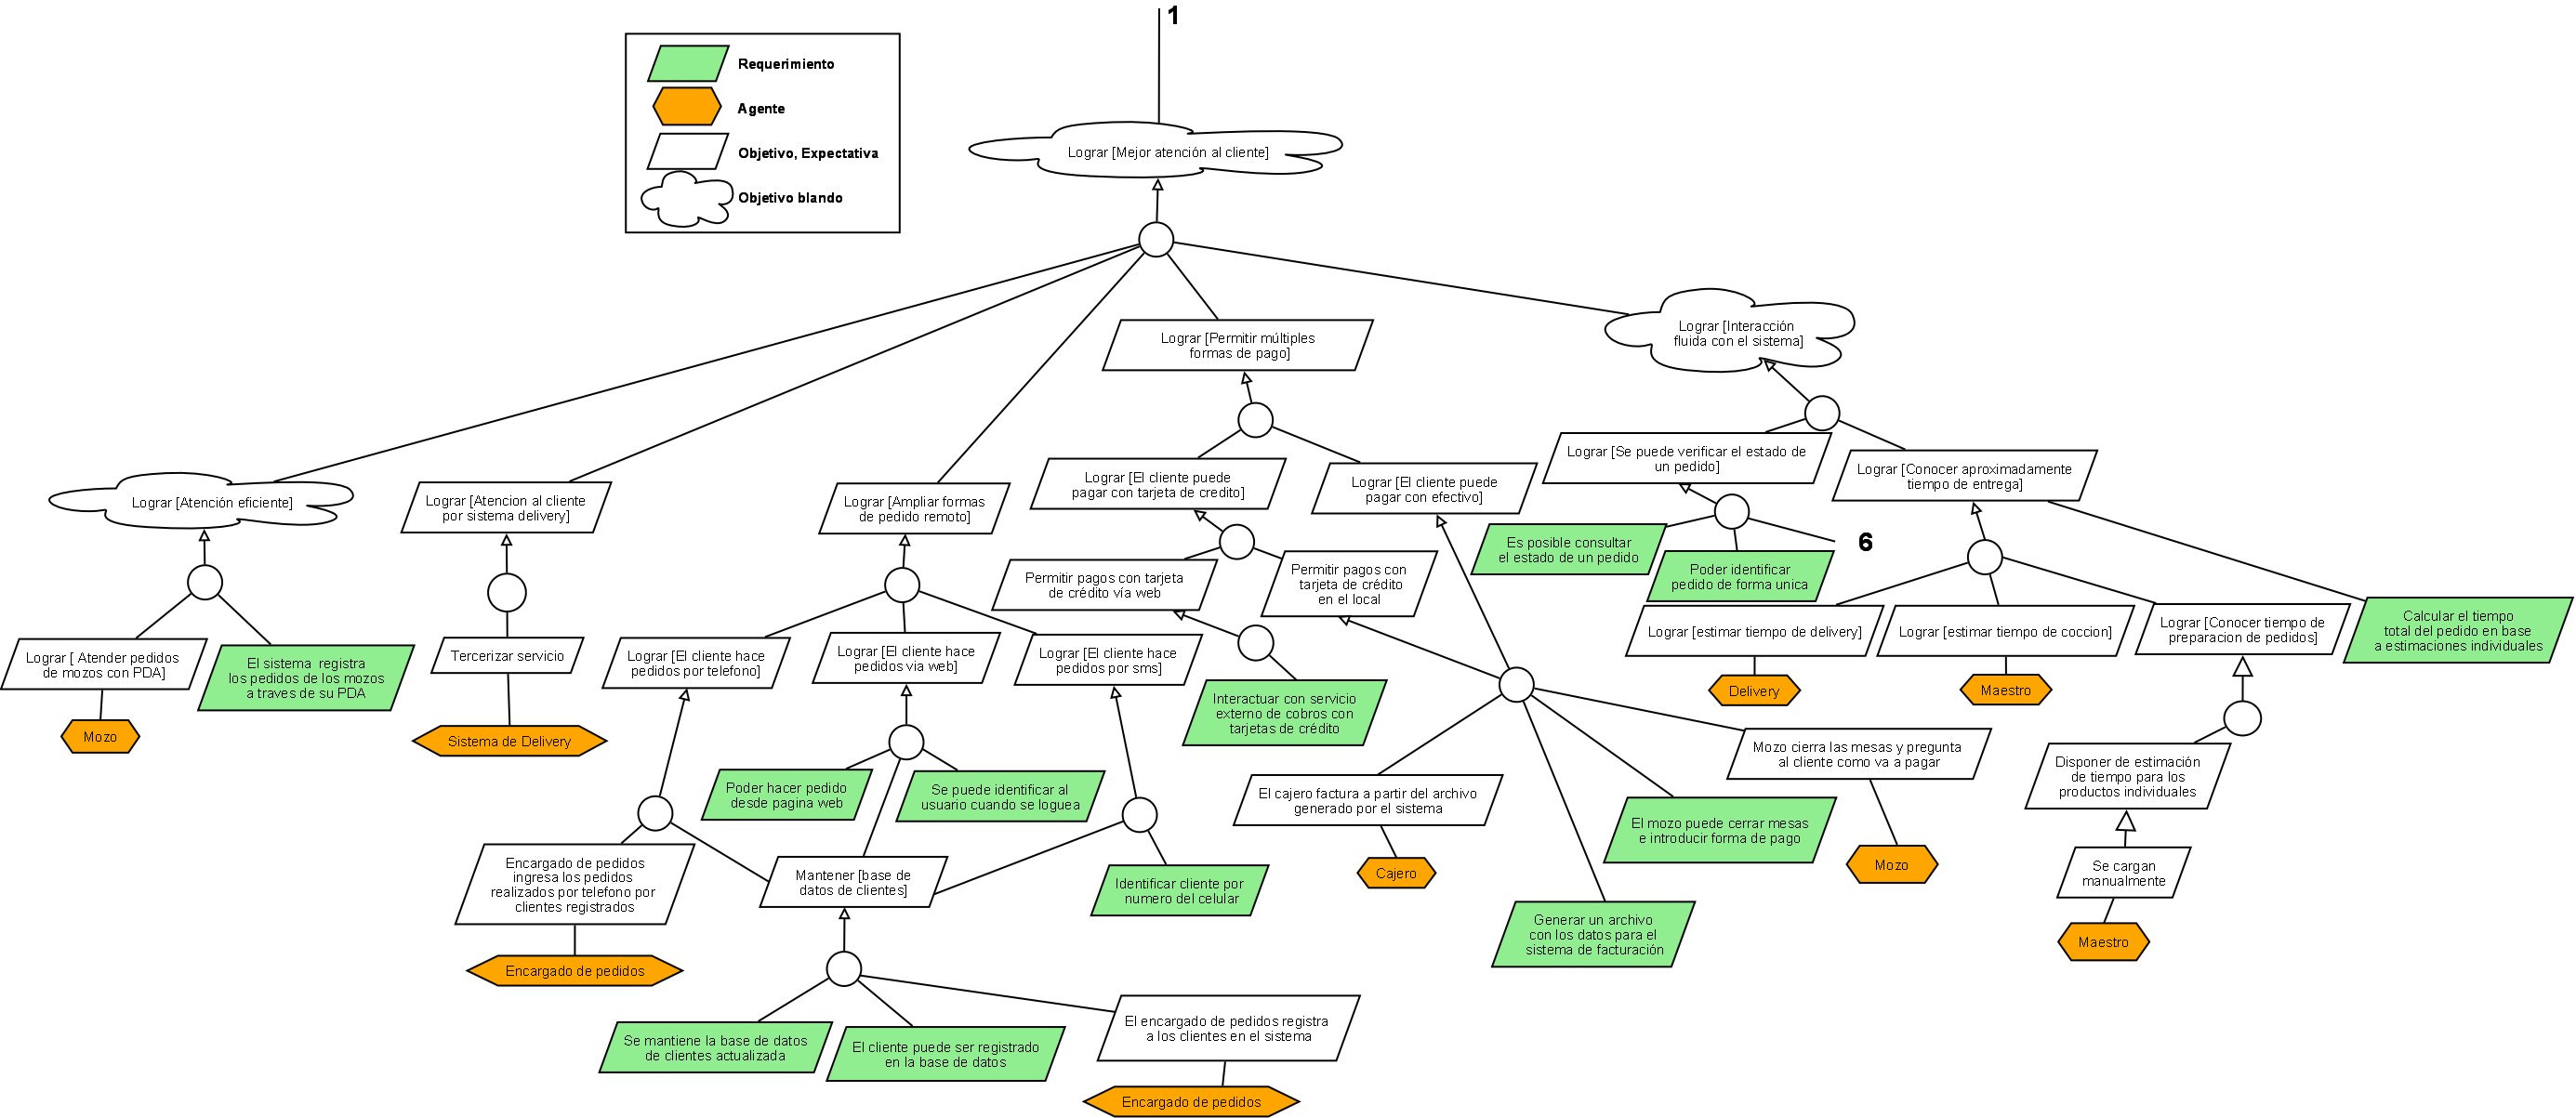
\includegraphics[height=16cm]{./figuras/DiagramaObjetivos1.png}
\end{figure}
\end{landscape}

\desreq{El sistema registra los pedidos de los mozos a trav�s de sus PDA}
{Funcional}
{Importante}
{Cuando un mozo toma un pedido desde una mesa, este puede ingresarlo al sistema utilizando una computadora de mano. Estos pedidos quedan registrados en el sistema.}
{Contribuye a lograr una atenci�n eficiente de los clientes locales.}

\desreq{Poder hacer pedido desde p'agina web}
{Funcional}
{Importante}
{El usuario tiene que poder ingresar un pedido desde la interfaz que brinda la p�gina web de la pizzer�a.}
{Para ampliar las formas de venta, el cliente debe poder hacer pedidos v�a web.}

\desreq{Se puede identificar al usuario cuando se loguea}
{Funcional}
{Importante}
{Es necesario poder identificar al usuario que quiere utilizar algun servicio de la pizzeria v�a web. Para ello tendr� asignado un usuario y una contrase�a para ingresar a su cuenta.}
{Cada usuario tendr� una cuenta, que utilizar� para realizar pedidos y revisar el estado de los mismos. Esto se requiere para poder proveer una mejor atenci�n a los clientes.}

\desreq{Se mantiene la base de datos de clientes actualizada}
{Funcional}
{Importante}
{Una base de datos actualizada es necesaria para poder tener informaci�n de los usuarios y permitirles realizar pedidos remotos.}
{Mantener una base de datos de clientes actualizada permite identificar de forma correcta a cada uno de ellos, y de esta manera registrar correctamente sus pedidos, permitiendo as� conocer informaci�n estad�stica sobre la distribuci�n de los pedidos. Esta informaci�n puede servir para crear promociones efectivas y mejorar la atenci�n al cliente.}

\desreq{El cliente puede ser registrado en la base de datos}
{Funcional}
{Importante}
{Deber� ser posible que el encargado de pedidos registre nuevos usuarios que se lo piden ya sea personal o telef�nicamente. De esta forma acceder�n a la posibilidad de realizar pedidos remotos.}
{Ayuda a mantener la base de datos de los clientes actualizada, permitiendo recibir pedidos remotos.}

\desreq{Identificar al cliente por su n�mero de celular}
{Funcional}
{Importante}
{An�logamente al caso Web, para poder hacer un pedido v�a SMS es necesario poder identificar el n�mero del celular que 
env�a el mensaje, y que �ste corresponda con alg�n cliente que se encuentre registrado en el sistema.}
{Contribuye a brindar el servicio de pedidos v�a SMS, ampliando las formas de pedido, lo que hace que se mejore la atenci�n a los clientes.}

\desreq{Interactuar con servicio externo de cobros con tarjeta de cr�dito}
{Funcional}
{Importante}
{El sistema debe ser capaz de interactuar con algun servicio externo tipo PayPal para permitir que un usuario realice el pago de su pedido utilizando una tarjeta de cr�dito.}
{Contribuye a tener una mayor variedad formas de pago, dejando que el cliente opte por la opci�n que m�s le convenga.}

\desreq{Generar un archivo con los datos para el sistema de facturaci�n}
{Funcional}
{Importante}
{Cuando se completa un pedido que deber� ser entregado por el delivery (cuando se encuentra en estado Listo, cocinado y con las bebidas), el sistema genera un archivo con los datos necesarios para realizar la factura cuando el cajero lo crea adecuado.}
{Contribuye a brindar la funcionalidad de pagos en efectivo o con tarjeta de cr�dito por parte de los clientes, interactuando con el sistema de facturaci�n existente.}

\desreq{El mozo puede cerrar mesas e introducir forma de pago}
{Funcional}
{Importante}
{Cuando se cierra una mesa, el mozo que la atiende debe preguntarle al cliente que forma de pago untilizar� e indicarselo al sistema.}
{Este requerimiento contribuye a permitir diferentes formas de pago.}


\begin{landscape}
\begin{figure}
\centering
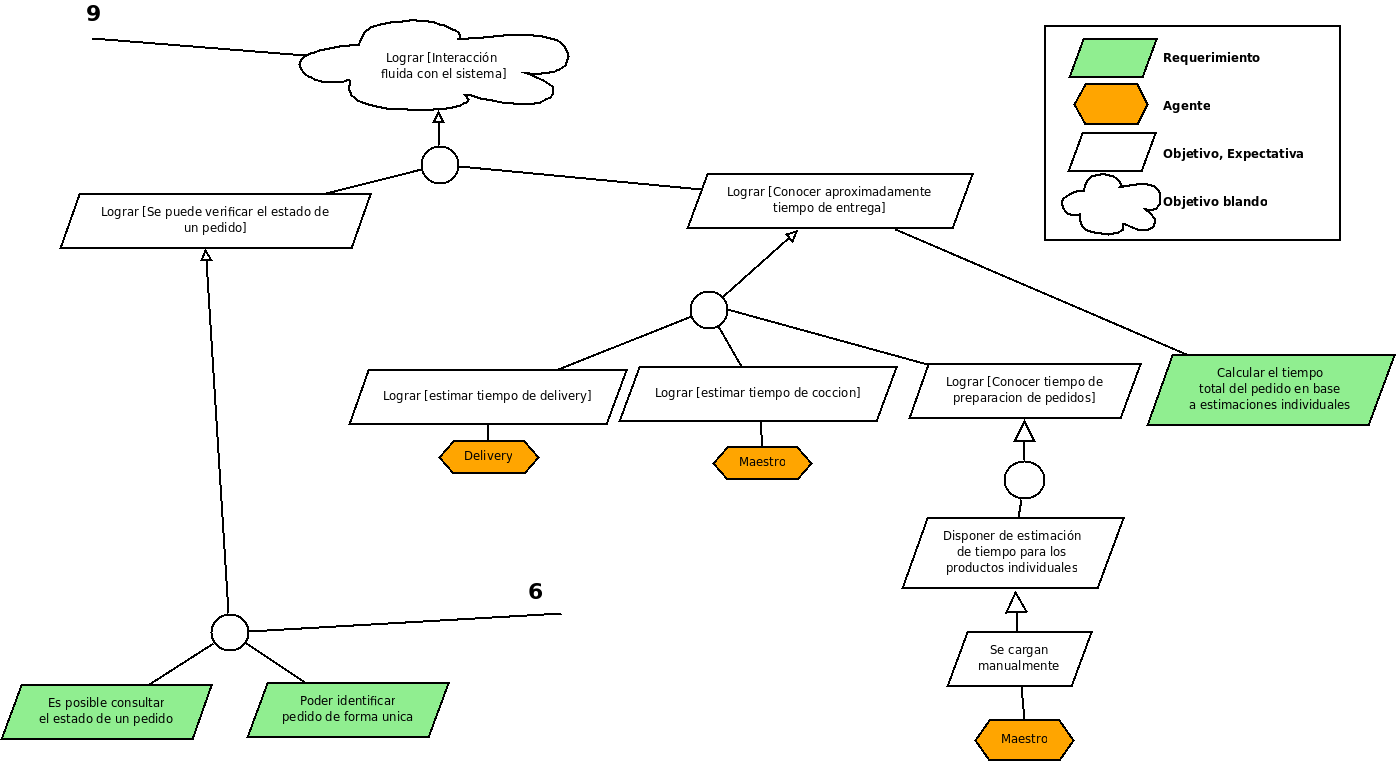
\includegraphics[height=12cm]{./figuras/DiagramaObjetivos5.png}
\end{figure}
\end{landscape}

\desreq{Es posible consultar el estado de un pedido}
{Funcional}
{Importante}
{Tanto un cliente como el encargado deben tener la posibilidad de consultar el estado de un pedido en cualquier momento. Para el caso de un usuario, lo podr� hacer directamente a trav�s de la Web.}
{Contribuye a permitir la consulta del estado de un pedido, y a lograr una interacci�n fluida del sistema con el usuario.}

\desreq{Poder identificar un pedido de forma �nica}
{Funcional}
{Importante}
{Debe ser posible referenciar a un pedido ingresado al sistema de forma un�voca para fines diversos (consultas de estado, modificaciones, etc)}
{Teniendo una �nica forma de identificar un pedido, se puede brindar la opci�n al cliente de verificar el estado de su pedido de forma remota, lo que mejora la interacci�n del sistema con el usuario y brinda una mejor atenci�n.}

\desreq{Calcular tiempo total del pedido en base a estimaciones individuales}
{Funcional}
{Importante}
{Los tiempos individuales para los productos deben usarse para poder estimar el tiempo de un pedido teniendo en cuenta la cola
de producci�n, la politica de asignaci�n, etc.}
{Se desea estimar el tiempo de preparaci�n de los pedidos, para contribuir a una mejor atenci�n de los clientes.}


\section{Casos de Uso}

\subsection{Diagrama de Casos de Uso}
\begin{figure}[H]
\centering
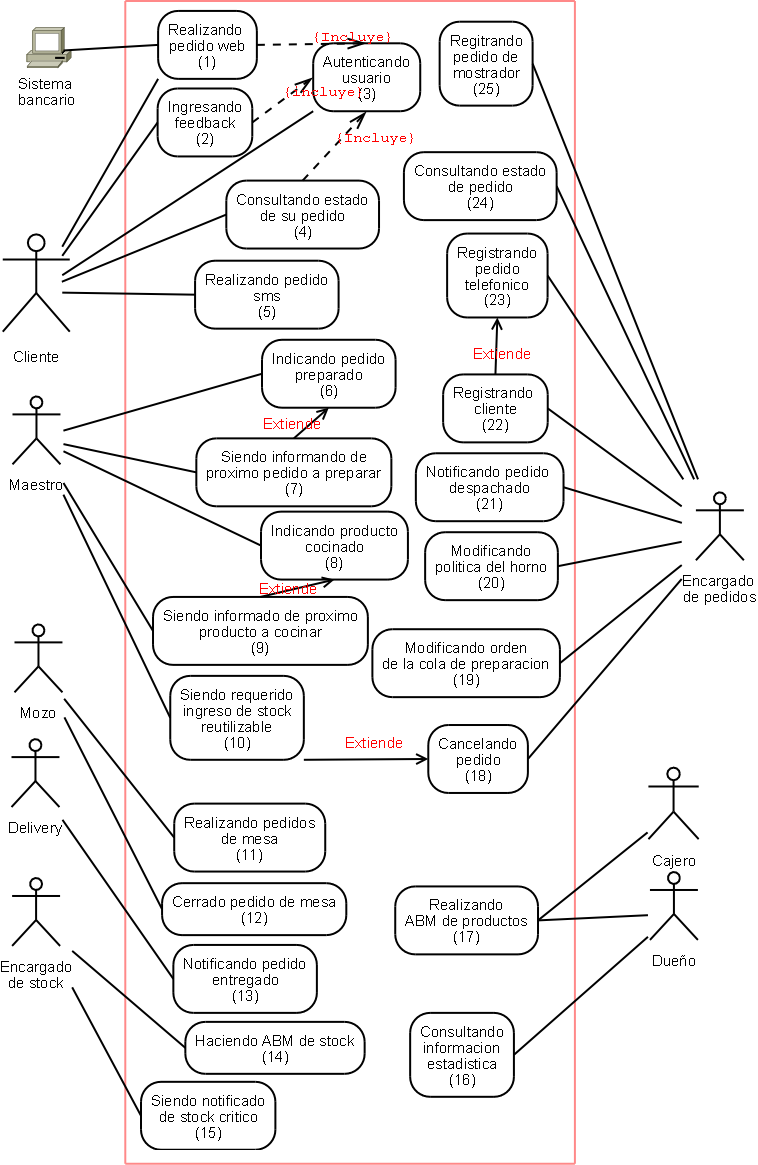
\includegraphics[height=21cm]{./figuras/casosdeuso.png}
\end{figure}

%%%%%%%%%%%%%%%%%%%%%%%%%%%%%%%%%%%%%%%%%%
% plantilla para casos de uso %%%%%%%%%%%%
%%%%%%%%%%%%%%%%%%%%%%%%%%%%%%%%%%%%%%%%%%
%\op{agrego una operacion en contexto normal}{y ahora su contexto de excepcion}
%\op{agrego otra}{lo malo es q no se numeran solas}
%\cu{nombre del caso de uso}{actor relacionado}{requerimiento}{pre}{pos}
%\oplist={} vacio la lista para otro caso de uso
%\cu{hola}{colo}{trolo}{fonolo}{rqqq}
%

\subsection{Descripci�n de Casos de Uso}
% Realizando pedido web
\op{1. INCLUYE autentificando usuario}{}
\op{2. Cliente selecciona de una lista los productos qu'e desea y su cantidad}{}
\op{3. El sistema brinda al cliente una estimaci'on de la demora del pedido y el costo total}{}
\op{4. El sistema pregunta al cliente si desea pagar con tarjeta de cr'edito o pagar en efectivo al delivery}{}
\op{5. El cliente elige forma de pago}{}
\op{6. Si el cliente eligi'o pagar en efectivo, ir al paso 14}{}
\op{7. Si el cliente eligi'o pagar con tarjeta y la tarjeta no se encuentra registrada, el sistema le pide al cliente que ingrese su n'umero de tarjeta, sino ir al paso 12}{}
\op{8. El cliente ingresa la tarjeta al sistema}{}
\op{9. El sistema pide al sistema bancario verificar si la tarjeta existe}{}
\op{10. Si la tarjeta existe, el sistema pide al sistema bancario verificar el monto}{10. Sino el sistema muestra un mensaje de error al cliente. Ir al paso 4}
\op{11. El sistema registra la tarjeta}{}
\op{12. El sistema pide al sistema bancario verificar si la tarjeta tiene fondos}{}
\op{13. Si el pago con tarjeta es posible, el sistema espera que el cliente confirme el pedido}{13. Sino Ir al paso 2}
\op{14. El cliente presiona el boton de enviar pedido}{}
\op{15. El sistema verifica si el pedido es viable (ver figura 4.3 FSM Chequeo de stock para m'as detalle)}{}
\op{16. Si el pedido es posible, ir al siguiente paso}{16. Si el pedido no es posible, se muestra mensaje de error al cliente indicando qu'e productos no estan disponibles. Ir al paso 2}
\op{17. Si el cliente eligi'o pagar con tarjeta, el sistema indica al sistema bancario que haga el pago}{}
\op{18 El sistema registra el pedido como ingresado}{}
\op{19. El sistema actualiza el stock}{}
\op{20. El sistema brinda al cliente un id de pedido para que luego consulte el estado del pedido si lo necesita}{}
\op{21. Fin CU}{}

\cu{Realizando pedido web}{Cliente, Sistema bancario}{3, 4, 5, 6, 24, 29, 30, 33}{TRUE}{Pedido registrado}{El cliente ingresa un pedido al sistema desde la pagina web (el diagrama de actividades de este caso de uso se puede ver en la secci'on de ingreso de pedidos remotos (4.2.1))}

%Ingresando feedback
\op{1. El cliente ingresa a la p�gina web de feedback}{}
\op{2. Se incluye CU autentificando usuario}{}
\op{3. Ingresa al apartado de feedback}{}
\op{4. Ingresa el n�mero de pedido}{}
\op{5. El sistema verifica que el n�mero de pedido corresponda con un pedido enviado por delivery a ese cliente, y obre el cual el mismo no halla ingresado feedback}{}
\op{6. Si el n�mero era valido, se muestra un formulario al usuario para que envia sus opini�n}{5. Si el n�mero no coincide se envia un mensaje de error al usuario}
\op{7. Fin CU}{}
\cu{Ingresando feedback}{Cliente}{8, 9}{TRUE}{Comentario ingresado}{Permite que el usuario envie al sistema su opini�n sobre un pedido recibido por delivery}

% Autenticando usuario
\op{1. El cliente ingresa su nombre de usuario en el campo correspondiente}{}
\op{2. El cliente ingresa su contrase�a en el campo correspondiente}{}
\op{3. El cliente presiona el boton de ingresar}{}
\op{4. El sistema valida los datos}{}
\op{5. Si los datos ingresados son validos, cliente autentificado}{5. Los datos no son validos, se muestra al cliente mensaje informativo y se le permite re ingresar los datos}
\op{6. Fin CU}{}
\cu{Autenticando usuario}{Cliente}{9, 24, 25}{TRUE}{Cliente logueado}{Autentificaci�n de un cliente web}

% Consultando estado de su pedido
\op{1. INCLUYE autentificando usuario}{}
\op{2. El cliente selecciona consultar estado de pedidos}{}
\op{3. El sistema muestra al cliente la lista de los pedidos del usuario pendientes de entrega cada uno con su estado correspondiente y demora estimada}{}
\op{4. Fin CU}{}
\cu{Consultando estado de su pedido}{Cliente}{32, 33, 34}{TRUE}{Se muestra el estado del pedido}{Permite al cliente ver en que estado se encuentran sus pedidos en un momento dado}

% Realizando pedido via SMS
\op{1. El cliente consulta el cat'alogo de c'odigos de producto y combos, publicados en la web del sistema junto con el formato que debe tener el mensaje}{}
\op{2. El cliente env'ia un mensaje al sistema con el pedido a solicitar}{}
\op{3. El sistema verifica si el n�mero desde donde proviene el mensaje est'a registrado con alg�n cliente}{}
\op{4. Si el n'umero no se encuentra registrado, el sistema responde al cliente sugiri'endole registrarse por tel'efono o personalmente y el pedido es descartado. Ir a Fin CU}{3. Si el n�mero est'a registrado pero el mensaje no corresponde con ning�n c�digo se notifica al cliente que el c�digo no es v�lido}
\op{5. El sistema verifica si es posible satisfacer el pedido (ver figura 4.3 FSM Chequeo de stock para m'as detalle)}{}
\op{6. Si es posible se ingresa el pedido al sistema y se envia al usuario un mensaje, notific'andole que su pedido est'a ingresado, el importe total, el tiempo de demora aproximado y el c'odigo de pedido para realizar consultas sobre el mismo}{6. Sino el sistema le env'ia un mensaje al cliente avis'andole que el pedido no podr'a ser satisfecho, informando adem'as qu'e producto/s no est'an disponibles}
\op{7. El sistema actualiza el stock}{}
\op{8. Fin CU}{}
\cu{Realizando pedido sms}{Cliente}{3, 4, 5, 6, 28, 30, 36}{TRUE}{Pedido ingresado al sistema}{El cliente hace un pedido via sms}

% Indicando pedido preparado
\op{1. El maestro indica al sistema que finaliz'o la preparaci'on del 'ultimo pedido que le pidi'o}{}
\op{2. El sistema registra el 'ultimo pedido que le orden'o preparar al maestro como preparado}{}
\op{3. Si hay pedido para preparar el sistema le informa que debe preparar a continuaci�n. EXTIENDE caso de uso Siendo informado de proximo pedido a preparar}{} 
\op{4. Fin CU}{}
\cu{Indicando pedido preparado}{Maestro}{8, 10, 13, 33}{El maestro tiene un pedido en preparaci�n}{El pedido se registra como preparado}{El maestro, luego de preparar un pedido, indica al sistema que el mismo est'a preparado (el diagrama de actividades de este caso de uso se puede ver en la secci'on de ingreso de pedidos remotos (4.2.1))}

% Siendo informado de proximo pedido a preparar
\op{1. El sistema indica al maestro preparar el primer pedido en la cola de pedidos a preparar y espera que el maestro confirme}{}
\op{2. El maestro indica al sistema que empezar'a a preparar la parte pedida}{}
\op{3. El pedido cambia su estado a ``en preparacion'' y sale de la cola de pedidos}{}
\op{4. Si hay m'as pedidos a preparar, ir a paso 1}{}
\op{5. Fin CU}{}
\cu{Siendo informado de proximo pedido a preparar}{Maestro}{8, 10, 13, 33}{La cola de pedidos a preparar no est'a vac'ia}{La parte de pedido comienza a prepararse}{El sistema le ordena al maestro que parte de pedido preparar}

% Indicando producto cocinado
\op{1. El maestro indica al sistema que finaliz'o la cocci'on de ciertas partes de un pedido}{}
\op{2. El sistema muestra al maestro un men'u de partes que deb'ian cocinarse y espera que el maestro indique la parte}{}
\op{3. El maestro indica al sistema qu'e parte finaliz'o la cocci'on}{}
\op{4. El sistema registra la parte como cocinada}{}
\op{5. El sistema verifica si la 'ultima parte cocinada completa el pedido}{}
\op{6. Si es as'i, el sistema registra al pedido como listo}{}
\op{7. Si hay productos para cocinar el sistema le informa al maestro que de debe poner a continuaci�n. EXTIENDE caso de uso Siendo informado de proximo producto a cocinar}{}
\op{8. Fin CU}{}
\cu{Indicando producto cocinado}{Maestro}{8, 11, 12, 14, 15}{True}{La parte de pedido se registra como cocinada}{El maestro, luego de cocinar una parte de un pedido, indica al sistema que la misma est'a cocinada  (este caso de uso se relaciona con el diagrama de actividad al informar productos cocinados (secci'on 4.7 Cola de horno))}

% Siendo informado de proximo producto a cocinar
\op{1. El maestro pide al sistema que pedido debe cocinar a continuaci'on}{}
\op{2. El sistema indica al maestro una parte a cocinar}{}
\op{3. Si es la primera parte de un pedido, el sistema cambia el estado del mismo a ``en horno''}{}
\op{4. Fin CU}{}
\cu{Siendo informado de proximo producto a cocinar}{Maestro}{8, 11, 12, 14, 15}{La cola del horno no est'a vac'ia}{La parte comienza a cocinarse}{El sistema le ordena al maestro que parte de pedido debe cocinar  (este caso de uso se relaciona con el diagrama de actividad al informar productos cocinados (secci'on 4.7 Cola de horno))}

% Siendo requerido ingreso de stock reutilizable
\op{1. El sistema indica al maestro que el pedido en preparaci'on fue cancelado}{}
\op{2. El sistema pide al maestro que indique que parte de los insumos se puede reutilizar para reingresar al stock}{}
\op{3. El maestro ingresa las cantidades y tipo de los insumos reutilizables}{}
\op{4. El maestro confirma reingresar insumos}{}
\op{5. El sistema lo registra y actualiza el stock}{}
\op{6. Fin CU}{}
\cu{Siendo requerido ingreso de stock reutilizable}{Maestro}{3, 22}{Hay cancelaci'on de un pedido que est'a en preparaci'on}{Los insumos reutilizables son reingresados al stock}{Cuando el maestro esta preparando un pedido que es cancelado, este debe reingresar al sistema los insumos que no utiliz� en la preparaci�n}

% Realizando pedidos mesa
\op{1. El cliente informa al mozo lo que quiere pedir}{}
\op{2. El mozo marca en su PDA los productos que el cliente pide con sus respectivas cantidades}{}
\op{3. Cuando el cliente inform� todo el pedido, el mozo ingresa el pedido}{}
\op{4. El sistema verifica si el pedido es posible (ver figura 4.3 FSM Chequeo de stock para m'as detalle)}{}
\op{5. Si el pedido se puede tomar, el sistema genera el id del pedido, calcula el costo total, y si no era de solo bebidas, estima el tiempo del mismo, y muestra estos datos al mozo}{5. Sino el sistema indica mediante un mensaje de error que producto/s no estaba/n disponible/s, y el mozo le comunica al cliente sobre la situaci'ion. Ir a paso 1}
\op{6. El sistema actualiza el stock}{}
\op{7. Fin CU}{}

\cu{Realizando pedidos mesa}{Mozo}{3, 4, 5, 6, 23, 30, 33}{TRUE}{El pedido de la mesa queda registrado}{El cliente del local hace un pedido a un mozo, quien ingresa el pedido (el diagrama de actividades de este caso de uso se puede ver en la secci'on de ingreso de pedidos locales (4.2.2))}

% Cerrando pedido de mesa
\op{1. El cliente llama al mozo}{}
\op{2. El cliente dice al mozo que va a pagar}{}
\op{3. El mozo selecciona el/los pedidos de la mesa, y pide al cliente forma de pago}{}
\op{4. El mozo ingresa la forma de pago que el cliente comunica y cierra la mea}{}
\op{5. Fin CU}{}

\cu{Cerrando pedido de mesa}{Mozo}{30, 31}{TRUE}{Se registra la forma de pago del pedido y se cierra la mesa}{Permite que el cliente le informe al mozo su forma de pago, que el mozo la registre y el pedido este listo para ser facturado}

% Notificando pedido entregado
\op{1. El delivery entrega el pedido al cliente}{1. Si es imposible entregar el pedido, el delivery env'ia un mensaje para que quede cancelado}
\op{2. El delivery envia un mensaje con el codigo del pedido}{}
\op{3. El sistema recibe el mensaje y el estado del pedido cambia a entregado}{}
\op{4. Fin CU}{}

\cu{Notificando pedido entregado}{Delivery}{8, 33}{True}{El pedido se registra como entregado}{Permite que el delivery mediante SMS informe inmediatamente la entrega o no entrega de un pedido}

% Haciendo ABM de stock
\op{1. El encargado de stock elige que operaci�n realizar}{}
\op{2. El sistema le pide al encargado de stock que ingrese el nombre o n'umero del insumo}{}
\op{3. El encargado de stock ingresa el nombre o el n'umero identificador}{}
\op{4.1. Si se trata de un alta ir a paso 6}{}
\op{4.2. Si se trata de una modificaci�n ir a paso 9}{}
\op{4.3. Si se trata de una baja ir a paso 9.}{}
\op{5. El sistema permite ingresar la cantidad y otros datos del insumo}{}
\op{6. El encargado de stock ingresa cantidad en stock del nuevo insumo y datos}{}
\op{7. El sistema agrega el insumo a la lista con su cantidad en stock y datos}{}
\op{8. Ir a Fin CU}{}
\op{9. El sistema verifica que el insumo exista en la lista de insumos}{}
\op{10. Si es asi, se sigue al siguiente paso}{Si el insumo no existe, el sistema produce un mensaje de error y se procede a Fin CU}
\op{11. Si se trata de se una baja de un insumo, el sistema elimina el insumo de la lista, sino se procede a paso 13}{}
\op{12. Ir a Fin CU}{}
\op{13. El sistema le pide al encargado de stock que ingrese la cantidad a aumentar o a quitar}{}
\op{14. El encargado de stock ingresa la cantidad en stock del insumo}{}
\op{15. El sistema modifica la cantidad en stock del insumo}{}
\op{16. Fin CU}{}

\cu{Haciendo ABM de stock}{Encargado de stock}{2}{TRUE}{El stock queda actualizado con las modificaciones}{Se puede hacer alta, baja y modificaci'on de insumos y kits comprados o caducados (los diagramas de m'aquina de estado explican un poco m'as en la secci'on 4.14 ABM de stock la relaci'on de este caso de uso con el caso de uso Siendo notificado de stock cr'itico)}

% Siendo notificado de stock critico
\op{1. El sistema detecta que la cantidad de un insumo es por debajo del nivel cr'itico}{}
\op{2. El sistema advierte al encargado de stock qu'e insumo es cr'itico hasta que este confirme que el mensaje le ha llegado}{}
\op{3. El encargado de stock confirma al sistema que el mensaje le lleg'o}{}
\op{4. Fin CU}{}

\cu{Siendo notificado de stock cr'itico}{Encargado de stock}{1}{Alg'un kit o insumo est'a por debajo del nivel cr'itico}{Surge una advertencia de stock cr'itico}{En caso de que el stock de algun producto quede por debajo de un nivel cr'itico, el sistema avisar'a al encargado de stock de esta situaci'on (los diagramas de m'aquina de estado explican un poco m'as en la secci'on 4.14 ABM de stock la relaci'on de este caso de uso con el caso de uso Siendo notificado de stock cr'itico)}

% Consultando informacion estadistica
\op{1. Si el due�o desea observar informaci�n estadistica sobre un producto ir a paso 2, sino ir a paso 6}{}
\op{2. El due�o le indica al sistema que requiere datos estad'isticos sobre un producto o pedido}{}
\op{3. El due�o ingresa el n'umero de producto o pedido sobre el cual necesita averiguar estad'isticas}{}
\op{4. El sistema verifica que el producto o pedido exista}{}
\op{5. Si es asi, el sistema imprime en pantalla los datos estad'isticos}{Sino se produce un mensaje de error y se procede a Fin CU}
\op{6. El due�o elige que estadisticas observar entre las disponibles (ver detalle en informaci�n estadistica)}{} %TODO: ver que este link lleve a alguna parte :)
\op{7. Cuando el due�o observo las estadisticas que deseaba, ir a fin CU}{}
\op{8. Fin CU}{}

\cu{Consultando informaci'on estad'istica}{Encargado/Due�o}{8}{TRUE}{Las estad'isticas son mostradas en pantalla}{El due�o puede consultar la informaci'on estad'istica sobre los productos y pedidos gestionados}

% Realizando ABM de productos
\op{1. El due�o o cajero eligen si desean hacer un alta, baja o modificaci�n}{}
\op{2. Si quieren hacer un alta, ingresan el nombre del producto, precio, ingredientes y tiempo de cocci�n y preparaci�n (que deben ser dichos al due�o o cajero por el maestro). Si terminaron ir a Fin CU, sino ir a 1}{}
\op{3. Si quieren hacer una baja, eligen hacer baja y el prducto que quieren dar de baja. Si terminaron ir a Fin CU, sino ir a 1}{}
\op{4. Si lo que quer�an es hacer una modificaci�n, pueden escoger el producto y modificar los datos del mismo. Si terminaron ir a Fin CU, sino ir a 1}{}
\op{5. Fin CU}{}

\cu{Realizando ABM de productos}{Cajero, Due�o}{7, 20, 21, 22, 34}{TRUE}{Se realizan las altas, bajas o modificaciones pedidas por el Due�o o cajero}{Permite ingresar nuevos productos a la carta de la pizzar�a, indicar tiempos estimados de cocci�n y preparaci�n, modificar precios y dar de baja productos}

% Cancelando pedido
\op{1. El cliente informa al encargado de pedido su nombre o nombre de usuario y el id de pedido, o el cliente informa al mozo que desea cancelar un pedido y el mozo informa al encargado de pedidos el deseo de la mesa de cancelar el pedido}{}
\op{2. El encargado ingresa al sistema el nombre proporcionado por el cliente y el id de pedido}{}
\op{3. Se verifica que el pedido no haya sido entregado}{3. Si ya fue entregado, no se puede cancelar. Ir a fin CU}
\op{4. El sistema verifica que el pedido exista y que el cliente haya hecho el pedido}{}
\op{5. Si el pedido existe y est'a en estado preparando, se deben reingresar los insumos reutilizables. EXTIENDE caso de uso Agregando insumos reutilizables}{}
\op{6. Fin CU}{}

\cu{Cancelando pedido}{Encargado de pedido}{19, 33}{Pedido no entregado}{Pedido cancelado}{Un cliente solicita cancelar un pedido, por tel'efono o personalmente, y el encargado de pedidos se encarga de esta cancelaci'on.} 

% Modificando orden de la cola de preparacion
\op{1. El encargado de pedido selecciona modificar cola de pedidos}{}
\op{2. Selecciona de la lista asigando a cada maestro un pedido y lo mueve hacia la posici�n deseada}{}
\op{3. Ingresa aceptar}{}
\op{4. Fin CU}{}

\cu{Modificando orden de cola de preparaci�n}{Encargado de pedidos}{33}{True}{Orden de preparaci�n modificado}{Permite que el encargado de pedidos modifique la cola de pedidos}

% Modificando politica del horno
\op{1. El encargado de pedidos selecciona modificar pol'itica de horno}{}
\op{2. El sistema muestra las pol'iticas posibles y espera que el encargado elija una}{}
\op{3. El encargado elige una pol'itica}{}
\op{4. Si el encargado eligi'o la pol'itica de cola normal, el sistema registra que la pol'itica de horno a usar ser'a cola. Ir a Fin CU}{}
\op{5. Si el encargado eligi'o la pol'itica de colas con sector 'agil, el sistema le pide que ingrese cuales son los m'odulos 'agiles}{}
\op{6. El encargado ingresa los m'odulos 'agiles}{}
\op{7. El sistema registra que la pol'itica de horno a usar ser'a cola con sector 'agil}{}
\op{8. Fin CU}{}

\cu{Modificando pol'itica del horno}{Encargado de pedidos}{14}{No hay pedidos hechos}{Pol'itica de cola modificada}{El encargado de pedidos modifica la pol'itica de cola del horno. Este caso de uso se lleva a cabo cuando inicia el sistema}

% Notificando pedido despachado
\op{1. El encargado de pedidos selecciona al pedido que se va a despachar de entre los pedidos listos}{}
\op{2. Si el pedido era para delivery, el pedido pasa a estado enviado y se despachar'a a cargo del delivery}{}
\op{3. Si el pedido era para el local, el pedido pasa a estado finalizado y se despachar'a a cargo del mozo para que le entregue el pedido al cliente}{}
\op{4. Si el pedido era de mostrador, el pedido pasa a estado finalizado}{}
\op{3. Fin CU}{}

\cu{Notificando pedido despachado}{Encargado de pedidos}{8, 30}{El pedido debe estar listo}{Pedido marcado como despachado (o entregado en el caso de que sea local)}{Permite indicar que un pedido sali� con el delivery o que fue entregado al cliente en mostrador o por el mozo en la mesa}

\op{1. Si el cliente quiere actualizar sus datos ir a paso 7}{}
\op{2. El cliente solicita al encargado de pedidos registrarse (por via telef'onica o personalmente)}{}
\op{3. El encargado pide al cliente los datos:
\begin{itemize}
\item Nombre
\item Apellido
\item Direcci�n
\item Tel'efono
\item Usuario, password (opcional, solo necesario para hacer pedidos via Web)
\item E-Mail (opcional)
\item C�lular (opcional, solo necesario para poder hacer pedidos vis SMS)
\end{itemize}
}{}
\op{4. El cliente informa al encargado de pedidos sus datos}{}
\op{5. El encargado de pedidos registra estos datos en el sistema}{}
\op{6. El sistema registra el usuario en la lista de usuarios, ir a fin CU}{}
\op{7. El encargado de pedidos verifica los datos del usuario}{}
\op{8. El usuario indica que datos modificar, y con que valores}{}
\op{9. El encargado ingresa dichos datos}{}
\op{10. El sistema actualiza los datos}{}
\op{11. Fin CU}{}
\cu{Registrando cliente}{Encargado de pedidos}{25, 26, 27, 28}{El cliente no esta registrado en el sistema}{El cliente esta registrado en el sistema}{El cliente desea registrarse en la pizzer'ia y el encargado de pedidos lo atiende y registra}

% Registrando pedido telefonico
\op{1. El cliente llama al n'umero telef'onico de la pizzer'ia y lo atiende el encargado de pedidos}{}
\op{2. El encargado le pide al cliente sus datos de identificaci'on}{}
\op{3. El cliente informa al encargado de pedidos sus datos}{}
\op{4. El encargado indica al sistema que desea ingresar un pedido y luego ingresa los datos del cliente al sistema}{}
\op{5. El sistema verifica si el cliente est'a registrado}{}
\op{6. Si el cliente est'a registrado, el sistema muestra al encargado el perfil del cliente}{6. Sino el encargado de pedidos le sugiere al cliente la posibilidad de registrarse. Si el cliente no lo desea entonces ir a fin CU, sino se procede a registrarlo (EXTIENDE Registrando cliente e ir a paso 9 )} 
\op{7. El encargado de pedidos verifica el tel'efono del cliente registrado con el tel'efono desde el cual cliente est'a llamando}{}
\op{8. Si el tel'efono registrado no coincide con el tel'efono desde el cual est'a llamando pero el cliente tiene usuario y clave, el encargado le pide al cliente que este indique usuario y clave y verifica}{8. Si el tel'efono registrado no coincide con el tel'efono desde el cual el cliente est'a llamando y el cliente no tiene usuario y clave informar que no es posible tomar el pedido e ir a Fin CU}
\op{9. El encargado de pedidos indica al cliente que le dicte el pedido}{}
\op{10. Una vez finalizado, el encargado de pedidos intenta ingresar el pedido al sistema}{}
\op{11. El sistema verifica si es posible satisfacer el pedido (ver figura 4.3 FSM Chequeo de stock para m'as detalle)}{}
\op{12. Si el pedido es posible y no es de solo bebida, el sistema estima el tiempo del mismo, calcula el costo total y el encargado se lo comunica al cliente, sino el sistema indica mediante un mensaje de error que producto/s no estaba/n disponible/s, para que el encargado se lo comunique al cliente. Ir a paso 9}{}
\op{13. Si era de solo bebida, se registra el pedido como listo y se calcula el costo total, se lo comunica al cliente}{}
\op{14. El sistema actualiza el stock}{}
\op{15. Si el pedido es mixto, el sistema pide al encargado de pedidos que asigne un horno}{}
\op{16. El sistema genera el identificador de pedido y notifica al encargado de pedidos sobre estos datos, para que el encargado se lo notifique al cliente}{}
\op{17. Fin CU}{}

\cu{Registrando pedido telef'onico}{Encargado de pedidos}{3, 4, 5, 6, 30, 33}{True}{Pedido ingresado al sistema}{El cliente quiere hacer un pedido por v'ia telef'onica, el encargado de pedidos lo atiende y luego de verificar los datos ingresa el pedido al sistema (el diagrama de actividades de este caso de uso se puede ver en la secci'on de ingreso de pedidos remotos (4.2.1))}

\op{1. El encargado de pedidos indica al sistema que desea consultar el estado de un pedido}{}
\op{2. El sistema pide al encargado que ingrese el identificador o cliente del pedido quiere consultar}{}
\op{3. El encargado de pedidos indica al sistema que pedido desea consultar}{}
\op{4. El verifica si el pedido existe}{}
\op{5. Si es asi, seguir al siguiente paso}{Sino, ir a Fin CU}
\op{6. Si el encargado pidi'o consultar un pedido identificando al cliente, el sistema mostrar'a toda la informaci'on de los pedidos pendientes de entrega del cliente}{}
\op{7. Si el encargado pidi'o consultar un pedido identificando al mismo mediante el identificador, el sistema mostrar'a toda la informaci'on correspondiente al pedido que tiene tal identificador}{}
\op{8. Fin CU}{}

\cu{Consultando estado de pedido}{Encargado de pedidos}{32, 33, 34}{TRUE}{Se muestra la informaci'on del pedido consultado}{El encargado le pide informaci'on al sistema sobre un pedido en particular o sobre el cliente que haya hecho el pedido}

% Registrando pedido de mostrador
\op{1. El cliente comunica al encargado de pedidos que desea hacer un pedido}{}
\op{2. El encargado pregunta si el cliente esta registrado}{}
\op{3. Si es asi el cliente da sus datos al encargado, si no el pedido se registrara sin cliente}{}
\op{4. El encargado indica al sistema que desea ingresar un pedido de mostrador}{}
\op{5. El encargado de pedidos indica al cliente que le dicte el pedido}{}
\op{6. Una vez finalizado, el encargado de pedidos intenta ingresar el pedido al sistema}{}
\op{7. El sistema verifica si es posible satisfacer el pedido (ver figura 4.3 FSM Chequeo de stock para m'as detalle)}{}
\op{8. Si el pedido es posible y tiene alguna empanada o pizza, el sistema estima el tiempo del mismo, calcula el costo total y el encargado se lo comunica al cliente, sino el sistema indica mediante un mensaje de error que producto/s no estaba/n disponible/s, para que el encargado se lo comunique al cliente. Ir a paso 5}{}
\op{9. Si solo tenia bebidas, el pedido se ingresa como listo y se calcula el total}{}
\op{10. El sistema actualiza el stock}{}
\op{11. Si el pedido es mixto, el sistema pide al encargado de pedidos que asigne un horno}{}
\op{12. El sistema genera el identificador de pedido y notifica al encargado de pedidos sobre estos datos, para que el encargado se lo notifique al cliente}{}
\op{13. El encargado pregunta forma de pago al cliente, e ingresa esa forma de pago en el sistema, a fin de que luego se pueda generar el archivo para el sistema de facturaci�n}{}
\op{14. Fin CU}{}

\cu{Registrando pedido mostrador}{Encargado de pedidos}{3, 4, 5, 6, 33}{}{Pedido ingresado al sistema}{El cliente quiere hacer un pedido en el local para llevar}
\subsection{Matriz de trazabilidad}

A continuaci�n presentamos una matriz donde se pueden observar las relaciones entre requerimientos y casos de uso.
Dicha tabla contiene en sus filas a los requerimientos y en sus columnas a los casos de uso. Se indica con una cruz cuando
un caso de uso contribuye a satisfacer un cierto requerimiento. Esto permite visualizar r�pidamente la completitud
del sistema en lo que a requerimientos refiere.

Es de notar que hay tres filas en la tabla que no tienen ning�n caso de uso asociado. Se trata de los requerimientos 16, 17 y 18, y
la raz�n de esta anomal�a es que los requerimientos afectan al modo de operaci�n de contingencia. Los casos de uso correspondientes
a este modo no se encuentran listados en esta secci�n, sino que se discuten m�s adelante en la secci�n \ref{alternativacontingencia}, y por tanto no
aparecen en esta tabla.

\begin{landscape}

\begin{tabular}{|c|c|c|c|c|c|c|c|c|c|c|c|c|c|c|c|c|c|c|c|c|c|c|c|c|c|}
\hline 
Requerimiento\textbackslash{}Caso de uso & 1 & 2 & 3 & 4 & 5 & 6 & 7 & 8 & 9 & 10 & 11 & 12 & 13 & 14 & 15 & 16 & 17 & 18 & 19 & 20 & 21 & 22 & 23 & 24 & 25\tabularnewline
\hline
\hline 
1 &  &  &  &  &  &  &  &  &  &  &  &  &  &  & X &  &  &  &  &  &  &  &  &  & \tabularnewline
\hline
\hline 
2 &  &  &  &  &  &  &  &  &  &  &  &  &  & X &  &  &  &  &  &  &  &  &  &  & \tabularnewline
\hline
\hline 
3 & X &  &  &  & X &  &  &  &  & X & X &  &  &  &  &  &  &  &  &  &  &  & X &  & X\tabularnewline
\hline
\hline 
4 & X &  &  &  & X &  &  &  &  &  & X &  &  &  &  &  &  &  &  &  &  &  & X &  & X\tabularnewline
\hline
\hline 
5 & X &  &  &  & X &  &  &  &  &  & X &  &  &  &  &  &  &  &  &  &  &  & X &  & X\tabularnewline
\hline
\hline 
6 & X &  &  &  & X &  &  &  &  &  & X &  &  &  &  &  &  &  &  &  &  &  & X &  & X\tabularnewline
\hline
\hline 
7 &  &  &  &  &  &  &  &  &  &  &  &  &  &  &  &  & X &  &  &  &  &  &  &  & \tabularnewline
\hline
\hline 
8 &  & X &  &  &  & X & X & X & X &  &  &  & X &  &  & X &  &  &  &  & X  &  &  &  & \tabularnewline
\hline
\hline 
9 &  & X & X &  &  &  &  &  &  &  &  &  &  &  &  &  &  &  &  &  &  &  &  &  & \tabularnewline
\hline
\hline 
10 &  &  &  &  &  & X & X &  &  &  &  &  &  &  &  &  &  &  &  &  &  &  &  &  & \tabularnewline
\hline
\hline 
11 &  &  &  &  &  &  &  & X & X &  &  &  &  &  &  &  &  &  &  &  &  &  &  &  & \tabularnewline
\hline
\hline 
12 &  &  &  &  &  &  &  & X & X &  &  &  &  &  &  &  &  &  &  &  &  &  &  &  & \tabularnewline
\hline
\hline 
13 &  &  &  &  &  & X & X &  &  &  &  &  &  &  &  &  &  &  &  &  &  &  &  &  & \tabularnewline
\hline
\hline 
14 &  &  &  &  &  &  &  &  & X &  &  &  &  &  &  &  &  &  &  & X &  &  &  &  & \tabularnewline
\hline
\hline 
15 &  &  &  &  &  &  &  & X & X &  &  &  &  &  &  &  &  &  &  &  &  &  &  &  & \tabularnewline
\hline
\hline 
16 &  &  &  &  &  &  &  &  &  &  &  &  &  &  &  &  &  &  &  &  &  &  &  &  & \tabularnewline
\hline
\hline 
17 &  &  &  &  &  &  &  &  &  &  &  &  &  &  &  &  &  &  &  &  &  &  &  &  & \tabularnewline
\hline
\hline 
18 &  &  &  &  &  &  &  &  &  &  &  &  &  &  &  &  &  &  &  &  &  &  &  &  & \tabularnewline
\hline
\hline 
19 &  &  &  &  &  &  &  &  &  &  &  &  &  &  &  &  &  & X &  &  &  &  &  &  & \tabularnewline
\hline
\hline 
20 &  &  &  &  &  &  &  &  &  &  &  &  &  &  &  &  & X &  &  &  &  &  &  &  & \tabularnewline
\hline
\hline 
21 &  &  &  &  &  &  &  &  &  & X &  &  &  &  &  &  & X &  &  &  &  &  &  &  & \tabularnewline
\hline
\hline 
22 &  &  &  &  &  &  &  &  &  &  &  &  &  &  &  &  & X &  &  &  &  &  &  &  & \tabularnewline
\hline
\hline 
23 &  &  &  &  &  &  &  &  &  &  & X &  &  &  &  &  &  &  &  &  &  &  &  &  & \tabularnewline
\hline
\hline 
24 & X &  & X &  &  &  &  &  &  &  &  &  &  &  &  &  &  &  &  &  &  &  &  &  & \tabularnewline
\hline
\hline 
25 &  &  & X &  &  &  &  &  &  &  &  &  &  &  &  &  &  &  &  &  &  & X &  &  & \tabularnewline
\hline
\hline 
26 &  &  &  &  &  &  &  &  &  &  &  &  &  &  &  &  &  &  &  &  &  & X &  &  & \tabularnewline
\hline
\hline 
27 &  &  &  &  &  &  &  &  &  &  &  &  &  &  &  &  &  &  &  &  &  & X &  &  & \tabularnewline
\hline
\hline 
28 &  &  &  &  & X &  &  &  &  &  &  &  &  &  &  &  &  &  &  &  &  & X &  &  & \tabularnewline
\hline
\hline 
29 & X &  &  &  &  &  &  &  &  &  &  &  &  &  &  &  &  &  &  &  &  &  &  &  & \tabularnewline
\hline
\hline 
30 & X &  &  &  & X &  &  &  &  &  & X & X &  &  &  &  &  &  &  &  & X &  & X &  & \tabularnewline
\hline
\hline 
31 &  &  &  &  &  &  &  &  &  &  &  & X &  &  &  &  &  &  &  &  &  &  &  &  & \tabularnewline
\hline
\hline 
32 &  &  &  & X &  &  &  &  &  &  &  &  &  &  &  &  &  &  &  &  &  &  &  & X & \tabularnewline
\hline
\hline 
33 & X &  &  & X & X & X & X &  &  &  & X &  & X &  &  &  &  & X & X &  &  &  & X & X & X\tabularnewline
\hline
\hline 
34 &  &  &  & X &  &  &  &  &  &  &  &  &  &  &  &  & X &  &  &  &  &  &  & X & \tabularnewline
\hline
\hline 
Requerimiento\textbackslash{}Caso de uso & 1 & 2 & 3 & 4 & 5 & 6 & 8 & 7 & 9 & 10 & 11 & 12 & 13 & 14 & 15 & 16 & 17 & 18 & 19 & 20 & 21 & 22 & 23 & 24 & 25\tabularnewline
\hline
\end{tabular}
\end{landscape}
\section{Modelo conceptual}
A continuacion presentaremos un diagrama de conceptos que pretende modelar los principales conceptos visibles en nuestra soluci�n. El mismo pretende brindar una visi�n completa de lo que el sistema puede observar

\begin{landscape}
\subsection{Diagrama}
\begin{figure}[H]
\centering
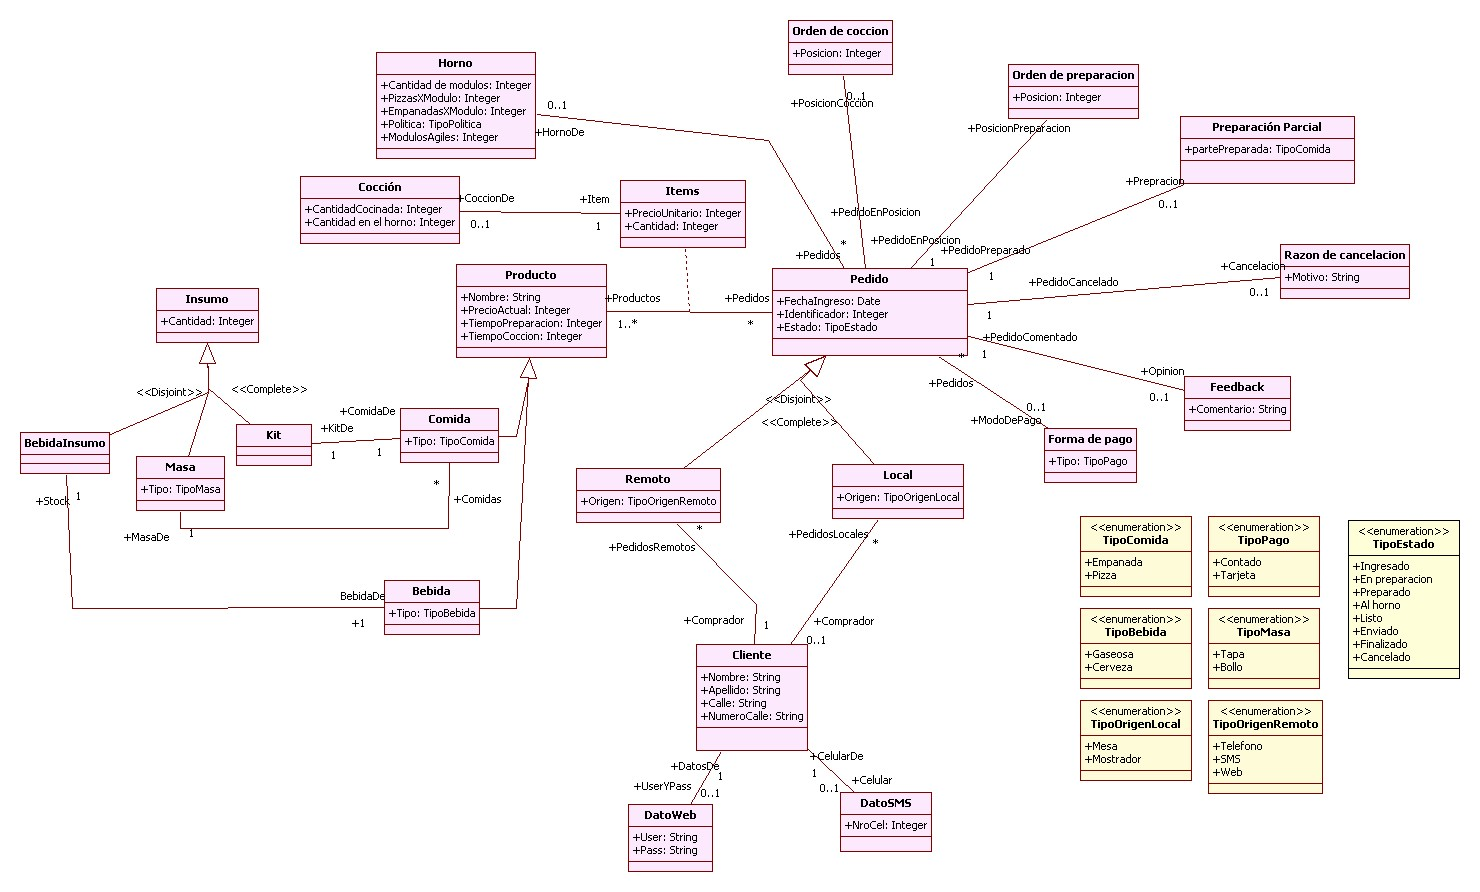
\includegraphics[scale=.5]{conceptos}
\end{figure}
\end{landscape}
%TODO: controlar esta descripci�n.
En el diagrama lo que observamos primeramente es que los pedidos son el concepto principal. Un pedido tiene una fecha de ingreso, un identificador unico en el sistema, y un estado. El pedido esta asociado a varios productos (Pizzas de muzzarella, napolitana, empanadas de carne, coca cola), y lleva una cierta cantidad de cada uno de ellos. Ademas estos productos se ligaron al pedido con un precio particular, que no necesariamente es el precio actual ya que los precios pueden cambiar.
Segun el estado que posea un pedido, esta relacionado con diferentes clases conceptuales. Por ejemplo un pedido cancelado, tiene una razon de cancelaci�n, un pedido ingresado tiene un orden en la cola de ingreso de pedidos a la cocina, el cual determina cuando pasa a ser preparado; una preparaci�n parcial esta relacionado con un pedido mixto que posee alguno de sus subproductos (pizzas o empanadas) ya preparados.

Los productos pueden ser comida (pizzas o empanadas) o bebidas. Para cada uno de ellos el sistema controla la cantidad disponible de insumos, en el caso de la comida es masa y kit, mientras que en el caso de las bebidas es la cantidad de bebidas en stock.

Los pedidos pueden ser locales o remotos segun su origen. Los pedidos remotos siempre tienen asociados a un cliente registrado, en cambio los pedidos locales podr�an estar vinculados a un cliente cuyos datos son desconocidos, por eso podemos considerar que pueden estar vinculados a 0 clientes. Un pedio remoto tiene necesariamente un forma de pago vinculada, mientras que un pedido local puede no tenerla, ya que si el cliente esta en una mesa, la forma de pago se decide cuando el cliente este dispuesto a pagar.

Un cliente registrado tiene cierta informaci�n basica, pero ademas puede registrar en alg�n momento otra informaci�n extra que lo habilita a hacer pedidos web, o pedidos SMS.

Cuando un pedido esta cocinandose, algunos de sus items estan en el horno, otros ya fueron cocinados. Esta informaci�n se encuentra en la clase cocci�n relacionada con los items de un producto.

Un pedido tiene uno o cero hornos porque el pedido podria ser exclusivamente de bebidas.
\subsection{Diccionario de datos} %TODO: no se q es

\subsection{Restricciones al MC en OCL}
\restr{Un pedido tiene un conjunto de estados valido}{}
\restr{Un pedido llega a los estado en orden valido}{}
\restr{Si el pedido no era en el local o ya fue entregado, entonces tiene una forma de pago}{}
\restr{Forma de pago tarjeta si y solo si pedido local o web}{}
\restr{Cliente tiene pedidos remotos web si tiene datos web y remotos sms si tiene numero de celular}{}
\restr{Si el pedido tiene solo pizzas y se esta preparando, empanadaspreparadas es true}{}
\restr{Si el pedido tiene solo empanadas y se esta preparando, pizzaspreparadas es true}{}
\restr{Un pedido tiene feedback si era remoto}{}
\restr{Cada estado se relaciona con un estado-pedido adecuado}{}
\restr{Todos los datos web son diferentes}{}
%TODO: q onda con los numeros?
\restr{Todos los numeros de celular son diferentes}{}
\restr{Todos los numeros de telefono son diferentes}{}
%TODO: dudoso
\restr{Para los pedidos de la misma fecha, los precios de sus items son iguales}{}
\restr{Un pedido tiene un horno si y solo si no es de solo bebidas}{}
\restr{Hay solo siete estados y tienen los nombres de los estados de pedido}{}
\restr{No hay dos pedidos con el mismo identificador}{}
\restr{}{}

\chapter{Aspectos particulares de la soluci�n}

\section{Ciclo de vida de un pedido}
Desde que el pedido es ingresado de alguna de las diversas maneras posibles, hasta que el cliente puede disfrutarlo, se suceden diversos estados, en lo que denominamos el ciclo de vida de un pedido.

Los estados en los que puede encontrarse un pedido una vez que ingres� al sistema son:
\begin{itemize}
\item Ingresado: El pedido pas� los chequeos necesarios, se determin� que es posible llevarlo a cabo con �xito y se ingres� al sistema, yendo a parar a una cola donde espera a que la cocina est� lista para prepararlo.
\item	En preparaci�n: El pedido ya fue recibido por la cocina y est� siendo preparado por un cocinero.
\item	Preparado: El pedido ya fue preparado en su totalidad y est� listo para ingresar al horno cuando haya lugar disponible.
\item	En el horno: El pedido (o al menos una de sus partes) est� en el horno.
\item	Listo: El pedido est� listo para ser entregado al cliente.
\item	Enviado: El pedido fue entregado al delivery para su entrega a domicilio.
\item	Finalizado: El pedido fue entregado con �xito (ya sea a la mesa o a domicilio).
\item	Cancelado: El pedido fue cancelado antes de su entrega.
\end{itemize}

En breve, un proceso ingresa al sistema cuando es requerido por un cliente por alg�n medio de comunicaci�n. Enseguida se indica a la cocina que el pedido debe ser preparado. Una vez completada la preparaci�n de la comida, los responsables de cocina lo indican al sistema que planifica de forma independiente la asignaci�n de lugares en los hornos. Finalmente, despu�s de que el pedido es horneado, se entrega a la mesa o al delivery seg�n corresponda. Por �ltimo cuando existe confirmaci�n de la entrega se marca el pedido como finalizado y se almacena con fines de registro. El pedido puede ser cancelado en cualquier punto (salvo despu�s de ser finalizado), con implicaciones varias en el sistema de control de stock.

Los estados presentados tienen utilidad para el sistema puesto que hay necesidad de indicar al cliente sobre el estado de su pedido. As�, se podr� indicar si un pedido est� siendo preparado o ya fue enviado al destinatario. Si bien para estos fines alcanza con 3 estados (preparando, enviando, finalizado), se agregan los dem�s con fines de control para el sistema. Adem�s, la granularidad m�s fina permite al sistema hacer predicciones y organizaciones m�s eficientes del uso de los recursos. Por ejemplo, al controlar los tiempos de preparaci�n por separado de los de horneado resulta m�s sencillo, en caso de un cuello de botella en la cocina, determinar cual es el factor limitante.


La figura \ref{cicloPedido} nos ilustra este ciclo de vida.

\begin{figure}[H]
\centering
\includegraphics[width=17cm]{./figuras/ciclo_pedido}
\caption{Ciclo de vida de un pedido}
\label{cicloPedido}
\end{figure}

A lo largo de las siguientes secciones se desarrollaran los diferentes aspectos de cada momento en la vida de un pedido, asi como otros aspectos relaciones a los pedidos.

\section{Ingreso de pedidos}
Los pedidos basicamente pueden ser remotos o locales. Los pedidos remotos se pueden realizar via telefonica, via web, o via sms.

Todos los pedidos tienen un �nico horno asignado, con la excepci�n de los pedidos de solo bebidas, a los que no se les asigna ning�n horno.

En todos los ingresos de pedidos, se realiza un chequeo de la disponibilidad del stock, a fin de evitar tomar pedidos que no se pueden satisfacer. La siguiente fsm presenta un modelo del control de stock para el ingreso de pedidos.

Supongamos que en la pizzeria hay hasta $k$ pedidos, hay $e$ tipos de empanadas y $i$ pizzas,
consideremos las siguientes variables:
stock pizza 1 : $[0...MAX_{STOCK}]$,
...
stock pizza i : $[0...Max_{STOCK}]$,
stock empanada 1 : $[0...MAX_{STOCK}]$,
...
stock empanada e : $[0...Max_{STOCK}]$,
stock stock bollo : $[0...MAX_{STOCK}]$,
stock stock tapas : $[0...Max_{STOCK}]$,

todas ellas comenznado con un valor SSTOCK constante.

pizza 1 1 : $[0...MAX]$
...
pizza 1 k : $[0...MAX]$
pizza 2 1 : $[0...MAX]$
...
pizza i k : $[0...MAX]$

donde pizza n m tiene cuantos kits de pizza del tipo n quiere el pedido m

de forma analoga tenemos las variables:

empanada 1 1 : $[0...MAX]$
...
empanada 1 k : $[0...MAX]$
empanada 2 1 : $[0...MAX]$
...
empanada e k : $[0...MAX]$

que guardan la cantidad de kits de empanadas de cada tipo que quiere cada pedido

pizzas 1 : $[0...MAX]$
...
pizzas k : $[0...MAX]$
indica cuantos bollos de pizza requiere cada pedido

empanadas 1 : $[0...MAX]$
...
empanadas k : $[0...MAX]$
indica cuantas tapas requiere cada pedido.

Entonces, la FSM de la figura \ref{fsmIngresoPedidos} modela el ingreso de pedidos para cada pedido $j = 0 ... k$

\begin{figure}[H]
\centering
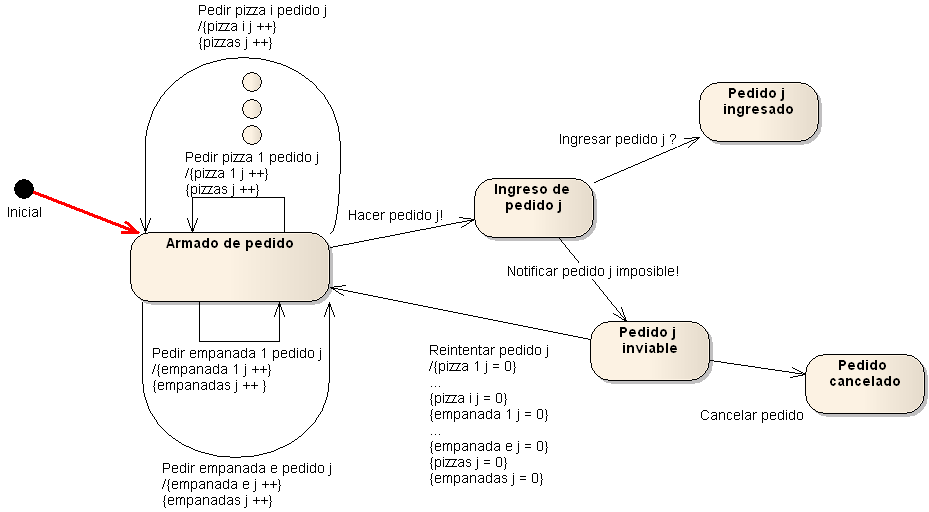
\includegraphics[scale=0.5]{./figuras/ingresoPedidos}
\caption{FSM ingreso de pedidos j}
\label{fsmIngresoPedidos}
\end{figure}

Lo que nos muestra dicha FSM es que durante el estado de armado de un pedido se seleccionan distintos productos con una cantidad dada de cada uno de ellos. Cuando el pedido esta armado, se intenta hacer el pedido. Entonces el mismo puede ser ingresado, o puede ser cancelado, pudiendo intentar hacer un pedido diferente o desistir.

En la figura \ref{fsmChequeoStock} vemos a la FSM que se encarga de controlar el stock para evitar el ingreso de pedidos no satisfacibles.

Esta fsm se encarga de decidir si el pedido se puede ingresar o no en base a la cantidad de stock y de productos necesarios.

La FSM que regula el ingreso de pedidos en base al stock se obtiene como:
FSM Ingreso Controlado de pedidos = FSM ingreso de pedidos 1 $||$ ... $||$ FSM ingreso de pedidos k $||$ FSM chequeo de stock

Analizando las trazas de la composici�n, podemos notar que cuando se hace un pedido, la decision de si se puede ingresar o no asi como el decremento del stock es un evento atomico, es decir no puede ocurrir que un pedido se este por ingresar y antes de decrementar el stock se ingresa otro. Situaci�n que podr�a hacer que se tomen pedidos y luego no se puedan satisfacer.
  
A continuaci�n detalleremos los distintos tipos de pedidos, asi como tambi�n describiremos las actividades propias de su ingreso

\begin{figure}[H]
\centering
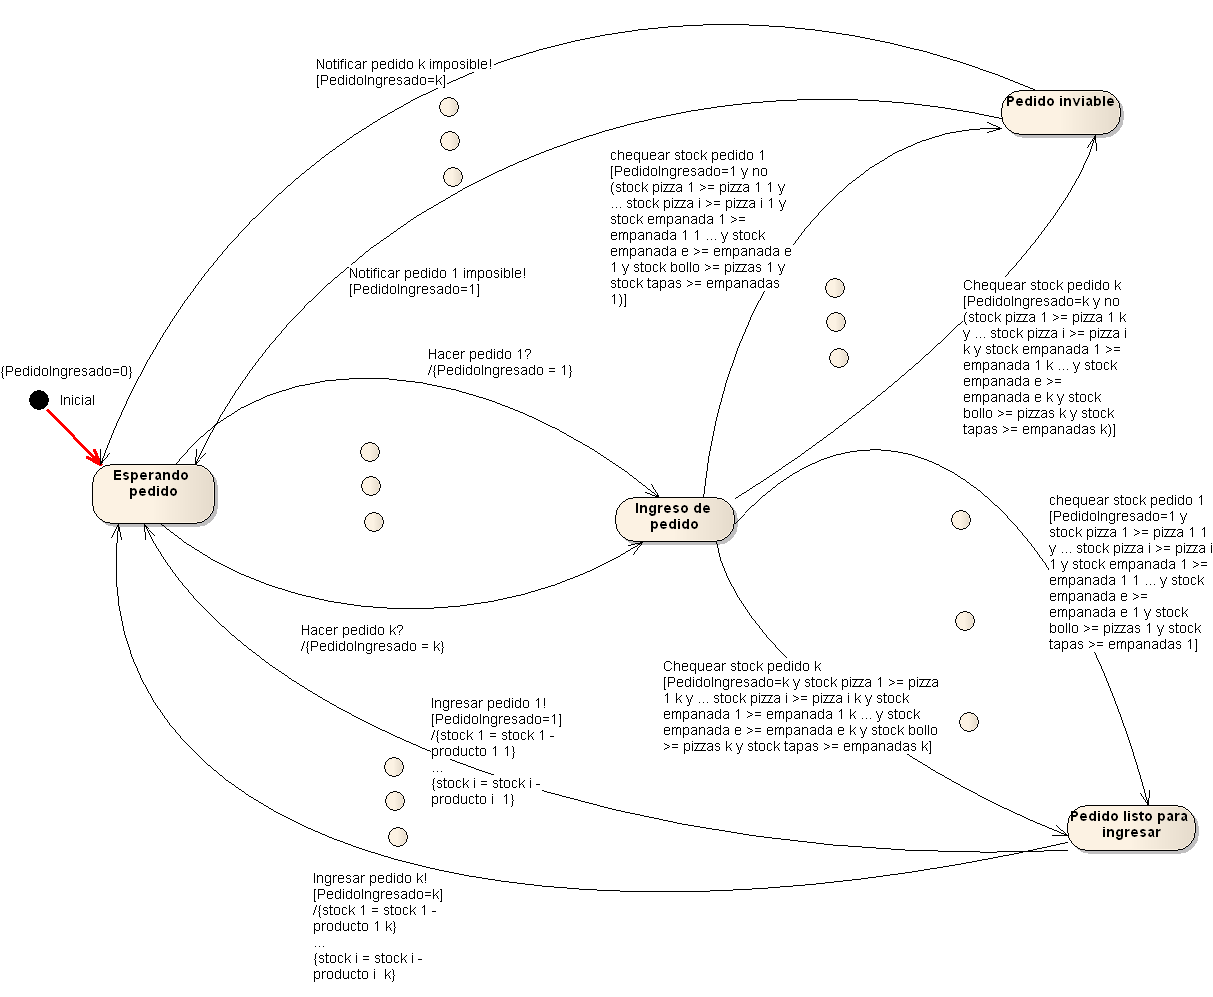
\includegraphics[scale=0.4]{./figuras/chequeoStock}
\caption{FSM chequeo de stock}
\label{fsmChequeoStock}
\end{figure}

\subsection{Pedidos remotos}
Los pedidos remotos requieren que los usuarios esten registrados en el sistema. Esto se hace por cuestiones de seguridad, a fin de evitar la realizaci�n de pedidos por parte de usuarios anonimos que podrian cancelar constantemente o dar direcciones falsas. La registracion de usuarios se realiza personalmente o telefonicamente. Decidimos no permitir regitro de usuarios via web, ya que consideramos que el m�todo no era del todo fiable (es facil crear usuarios ficticios y hacer pedidos en broma).

Si un usuario desea poder hacer pedidos v�a web, deber� elegir un nombre de usuario y una contrase�a al momento de registrarse, as� como proveer una direcci�n de mail. Si se desean hacer pedidos SMS, el usuario deber� brindar un n�mero de celular, al que se ``autoriza'' para efectuar pedidos a nombre de ese usuario. Para todo tipo de pedidos que involucren delivery, el usuario deber� registrar una direcci�n (aunque podr�a tener m�s de una, existe una �nica que es predeterminada).

A continuaci�n describiremos los procedimientos para la realizaci�n de pedidos remotos.

\subsubsection{Pedidos telefonicos}
El cliente que desee realizar un pedido telefonico debe llamar al n�mero de la pizzer�a. El encargado de pedidos es el responsable de atender los llamados telefonicos. El cliente debe brindar informaci�n de identificaci�n al encargado para permitir individualizarlo (nombre, direcci�n o nombre de usuario). El encargado corrobora entonces el n�mero desde el que est� llamando el usuario para verificar su identidad (eventualmente si llama desde otro n�mero puede identificarse con usuario y password si lo tuviera).

Si el usuario no estaba registrado, el encargado debe sugerirle la posibilidad de registrarse. Si el usuario no esta registrado y no desea registrarse, no se toma el pedido. %TODO: caso de uso chequear datos de usuario

Una vez autentificado el usuario, el mismo procede a dictar su pedido al encargado de pedidos. Una vez finalizado, el encargado de pedidos intenta ingresar el pedido al sistema, el cual se encarga de verificar si es posible satisfacer dicho pedido. En caso de no ser posible el sistema indicara mediante un mensaje de error que el pedido no fue posible de realizar e indicara que producto/s no estaba/n disponible/s. El cliente puede entonces dar un pedido diferente.

Si el pedido s� pod�a ser tomado, el sistema se encarga de registrar el pedido como ingresado. Se genera un identificador de pedido, se estima el tiempo del mismo y se calcula el costo total. Ademas si el pedido es mixto se brinda la posibilidad de que el encargado de pedidos asigne un horno. %TODO: caso de uso loco

\begin{figure}
\centering
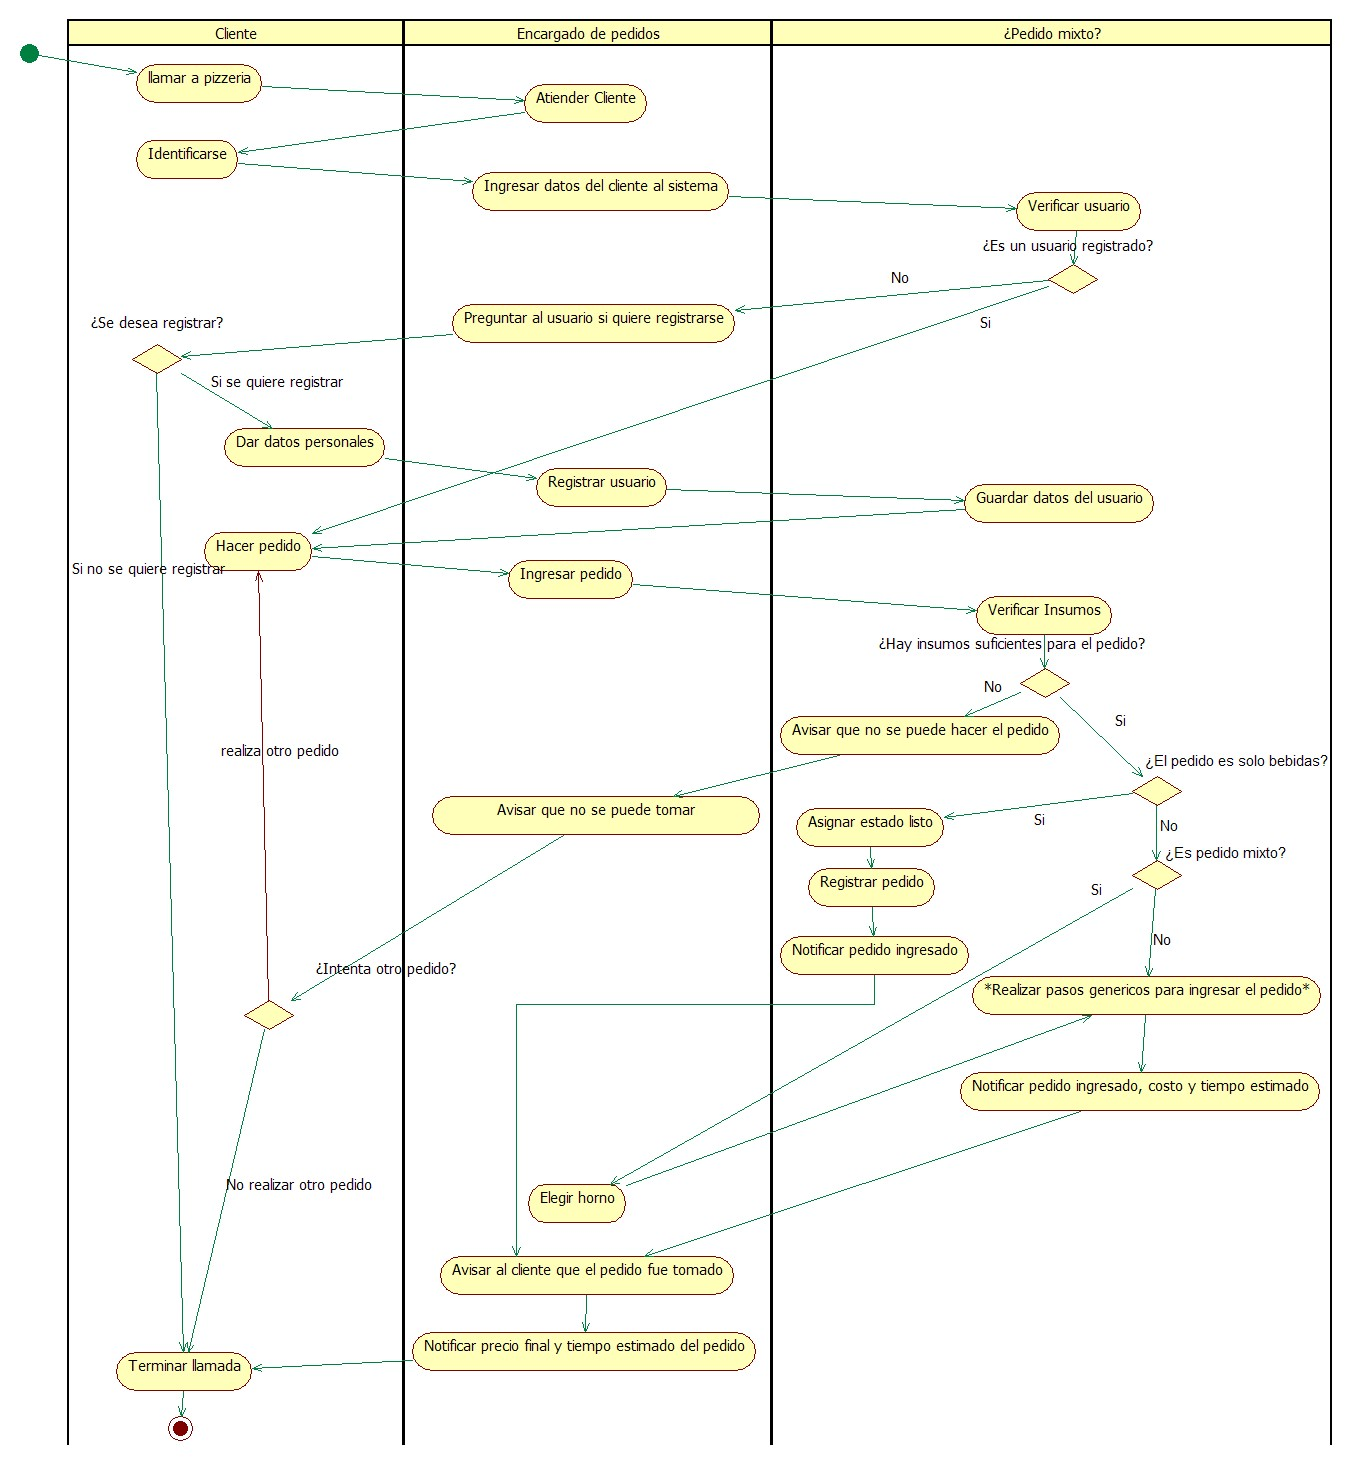
\includegraphics[height=19cm]{./figuras/diagramaActividadTelefono}
\caption{Diagrama de actividad del ingreso de un pedido telef�nico}
\end{figure}

%TODO: poner diagrama de actividad
%NOTA: estos casos de uso q aparecen son medio especificos del caso, tonces se podria hacer un diagrama aparte

\subsubsection{Pedidos web}
Para que los clientes puedan realizar pedidos via web, la pizzer�a contara con una p�gina web. El cliente que desee hacer un pedido por esta v�a debe ingresar a la p�gina y autentificarse con usuario y contrase�a.

Una vez autentificado, tendra la posibilidad de elegir ingresar pedido. Entonces podra elegir que productos desea y con que cantidad a partir de una lista en l�nea. Dicha lista solo contiene productos que est�n disponibles (los que ya est�n fuera de stock no se incluyen). Cuando marc� lo que deseaba puede ingresar el pedido. Entonces el sistema verifica la viabilidad del pedido, y en caso de no ser posible de realizar lo informa mediante un mensaje indicando que producto no se encuentra disponible. El cliente puede volver a ingresar un pedido diferente si lo desea.

En caso de que sea posible registrar el pedido, se estima el tiempo del mismo y se calcula el costo total. Esta informaci�n se muestra al usuario por pantalla. A continuaci�n se le permite al usuario elegir si prefiere pagar contra entrega al delivery o con tarjeta de cr�dito. Si la operaci�n con tarjeta falla, se muestra un mensaje de error y se permite al usuario reingresar los datos de la misma o cambiar de forma de pago. Hecho esto, se confirma todo el pedido.

Si entre la elecci�n de los productos y la confirmaci�n del pedido se acaba el stock de materias primas, se muestra un error y se vuelve a la pantalla de selecci�n de productos (esto deber�a ser muy raro). 

Una vez que el pedido fue ingresado, si se pagaba con tarjeta, se hace efectivo el cobro.

El pedido ser� encolado autom�ticamente tratando de balancear la carga de los hornos. 

\begin{figure}[H]
\centering
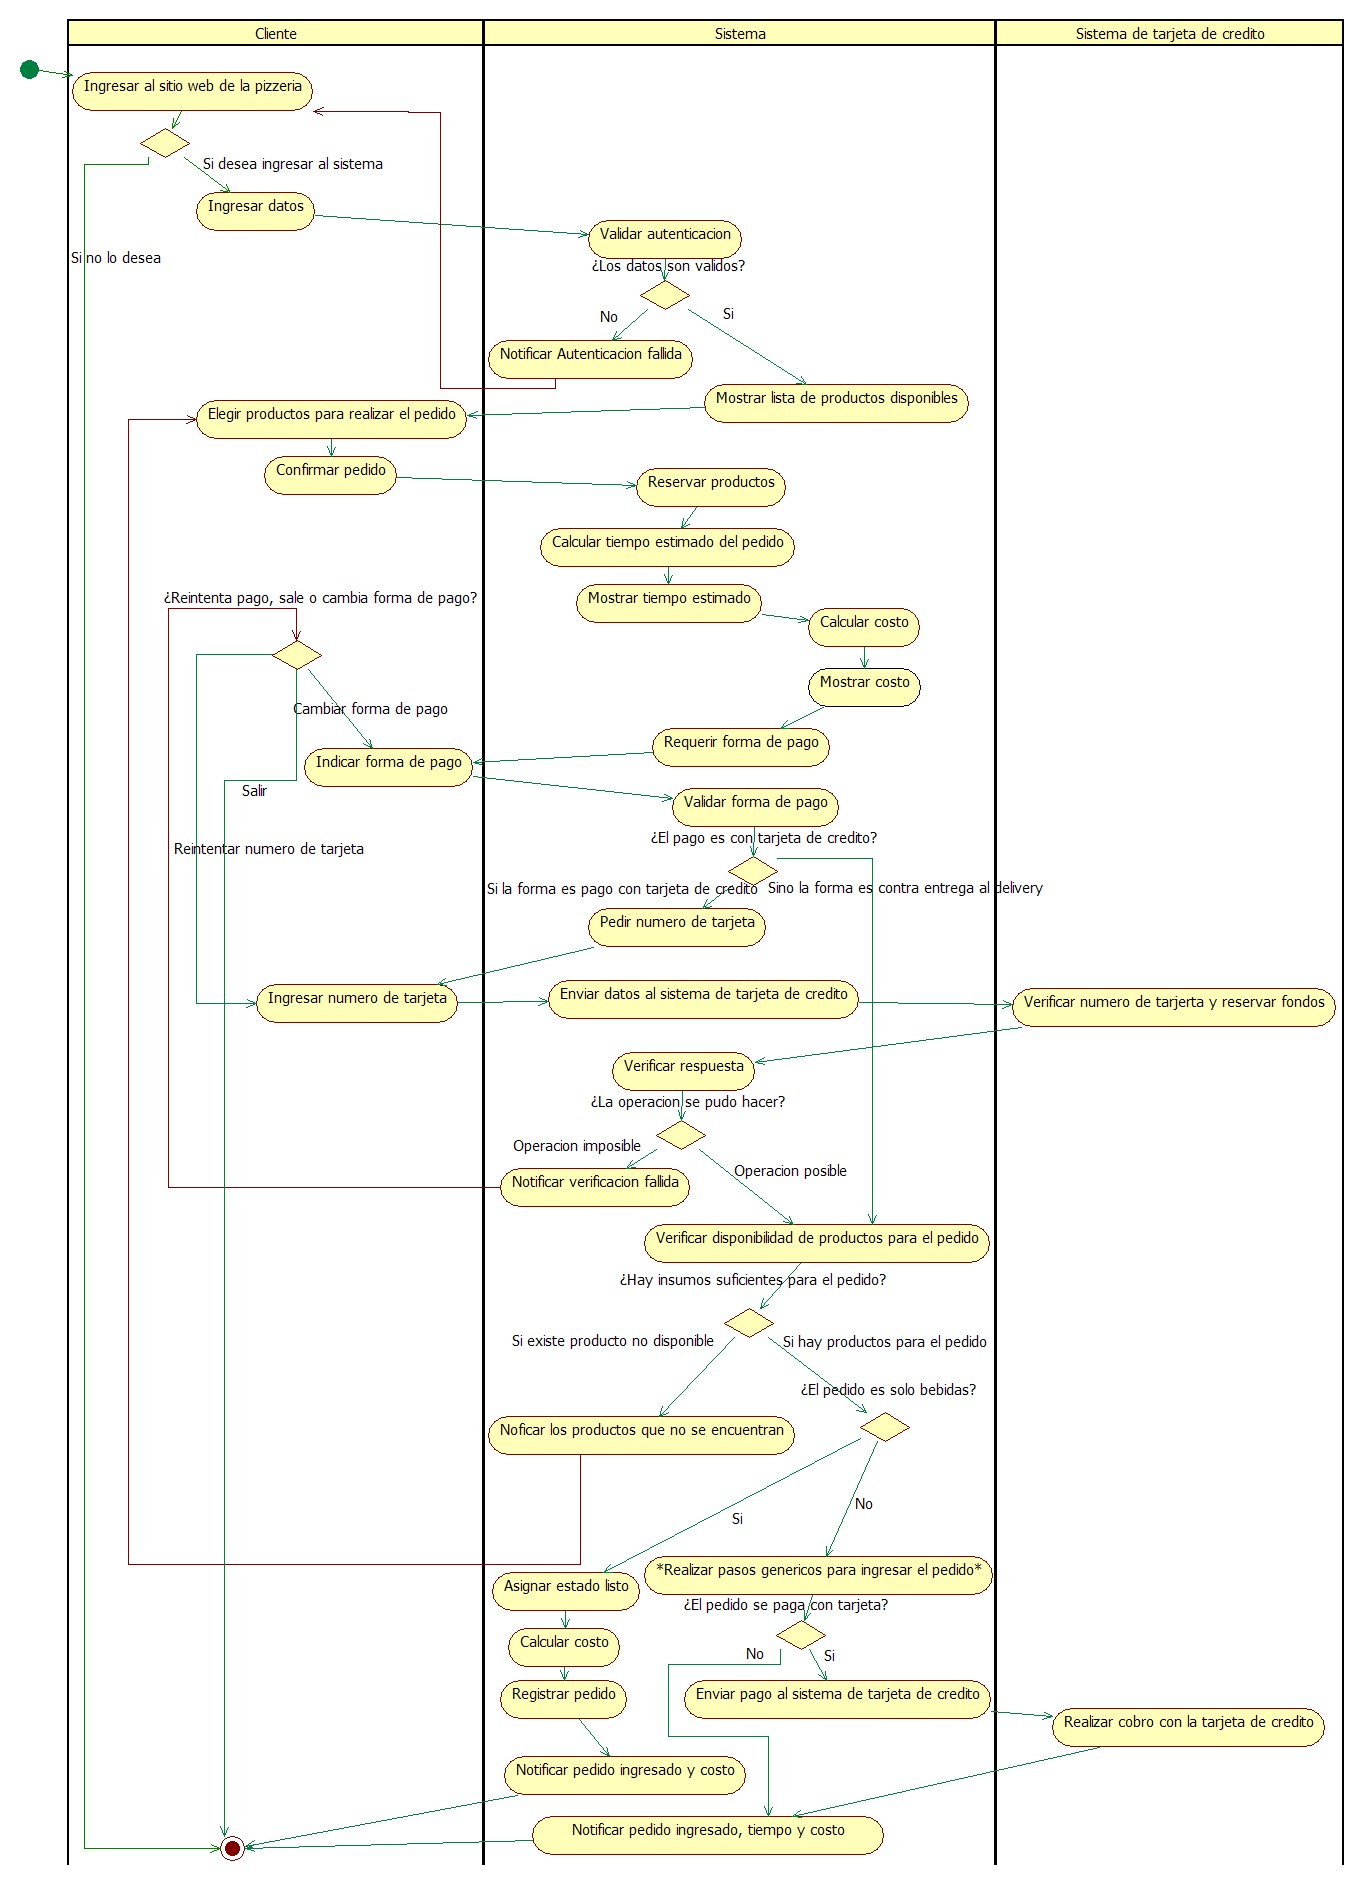
\includegraphics[height=23cm]{./figuras/diagramaActividadWeb}
\caption{Diagrama de actividad del ingreso de un pedido Web}
\end{figure}
%TODO:diagrama de actividad

\subsubsection{Pedidos SMS}
El cliente que desee realizar un pedido via sms debe enviar un mensaje al servidor sms de la pizzeria, junto con el pedido que quiere hacer. Si el celular no estaba registrado, el sistema descarta el pedido y le envia un mensaje sms al mismo sugiriendole registrarse por telefono o personalmente.

Para identificar los productos que desea pedir, el cliente cuenta con un cat�logo con c�digos de producto y de ``combos'' populares ya sea en papel o consultable via Internet.

El sistema verifica si es posible satisfacer el pedido. En caso de no ser posible el sistema le envia un mensaje al cliente para avisar que el pedido no podra ser satisfecho, indicando que producto no esta disponible. Si el pedido s� pod�a ser tomado, el sistema lo registra como ingresado, genera un identificador de pedido, estima el tiempo del mismo, calcula el costo total y luego de todo esto procede a enviarle un mensaje de respuesta de sms con esos datos al cliente. 

\begin{figure}[H]
\centering
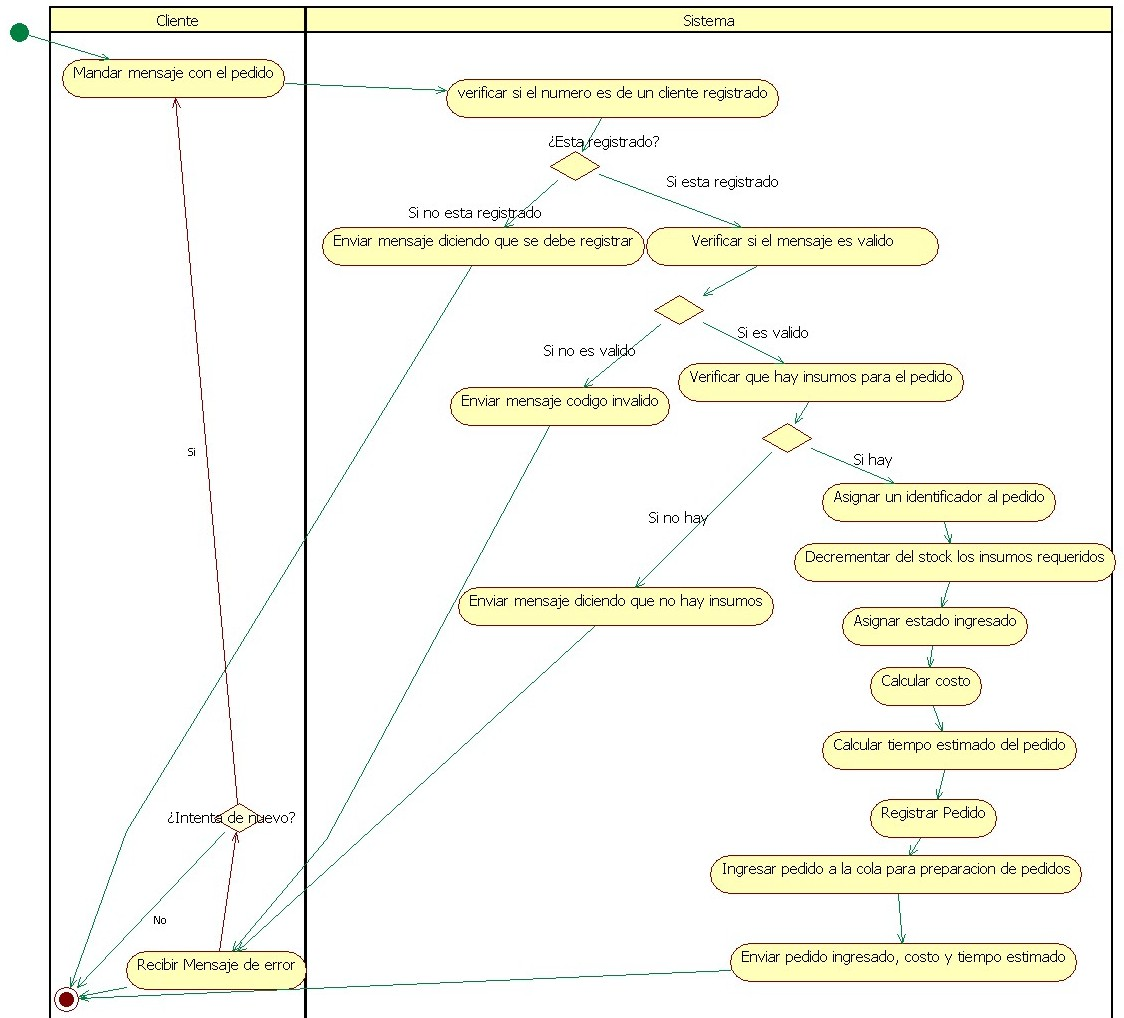
\includegraphics[height=17cm]{./figuras/diagramaActividadSMS}
\caption{Diagrama de actividad del ingreso de un pedido SMS}
\end{figure}

\subsection{Pedidos locales}
Los pedidos locales pueden realizarse a los mozos, quienes cuentan con una PDA para realizar el registro de los pedidos. Un cliente dicta su pedido a alg�n mozo, el cual marca los productos y sus cantidades en su PDA. una vez que el cliente dict� su pedido el mozo ingresa el pedido. El sistema verifica la factibilidad del mismo, si no es posible tomarlo, notifica al mozo para que informe de la situaci�n al cliente.

\begin{figure}[H]
\centering
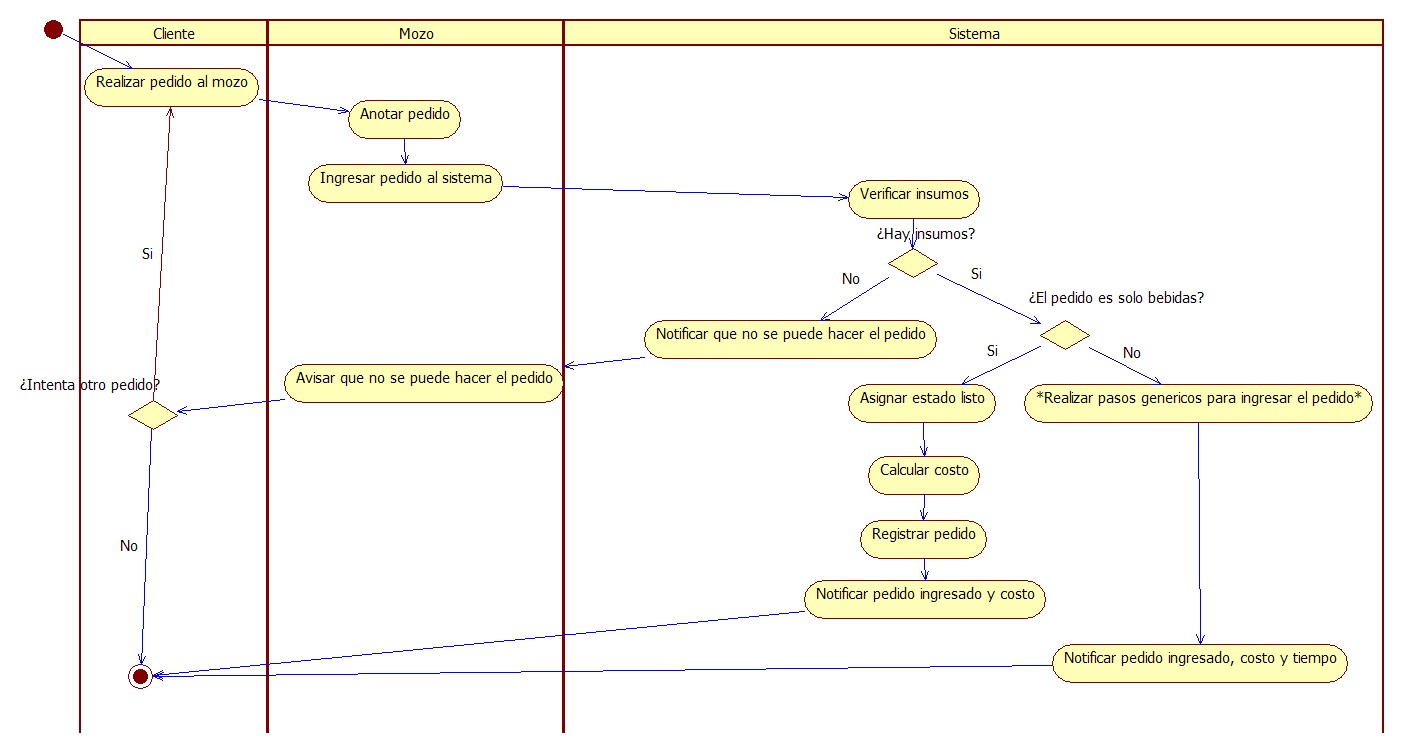
\includegraphics[height=9cm]{./figuras/diagramaActividadPedidoMozo.jpg}
\caption{Diagrama de actividad de toma de un pedido por parte del mozo}
\end{figure}

Si es posible ingresar el pedido el sistema genera el id del pedido, se estima el tiempo del mismo y se calcula el costo total. La asignaci�n del horno es tambi�n responsabilidad del sistema.

Por otro lado, un pedido local (de mostrador) se solicita al encargado de pedidos, quien registra los productos del pedido de manera similar a como registra los pedidos telefonicos, con le excepci�n de que en este caso pod�a no tener los datos del usuario.

%TODO:diagrama de actividad de ambos casos
\begin{figure}[H]
\centering
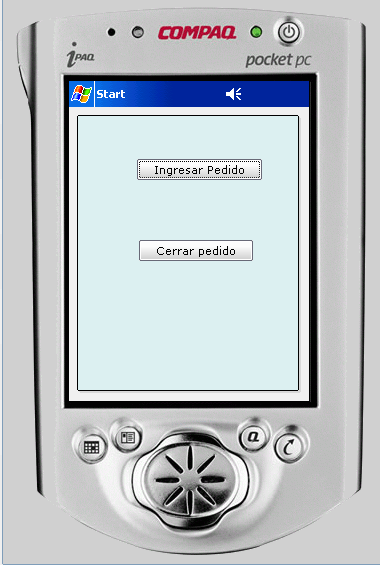
\includegraphics[height=12cm]{./figuras/pantallaBotonesMozo.png}
\caption{Interfaz del mozo para ingreso y cierre de pedido}
\end{figure}

\section{Registro de usuarios}
El registro de usuarios es responsabilidad del encargado de pedidos, y se realiza por via telefonica asi como tambi�n personalmente. 

Para registrar a un usuario el encargado de pedidos debe tomar los siguientes datos:
\begin{itemize}
\item Nombre
\item Apellido
\item Direcci�n
\item Telefono
\item Usuario, password (opcional, solo necesario para hacer pedidos via Web)
\item E-Mail (opcional)
\item C�lular (opcional, solo necesario para poder hacer pedidos vis SMS)
\end{itemize}

Una vez registrado el usuario puede en otro momento solicitar modificar algun dato, o agregar algun dato opcional.
%TODO: pantalla
Veamos operacionalmente como funciona el registro de un usuario:

La siguiente operaci�n permite registrar un usuario nuevo sin datos web ni SMS

\begin{funcion}{RegistroUsuario}{nombreC: String, apellidoC: String, CalleC: String, NumeroC: Integer}{}{}
   \precond{True}
   
   \poscond{Cliente.allinstances() $\rightarrow$ size() = Cliente@pre.allinstances() $\rightarrow$ size+1}
   
   \poscond{(Cliente.allinstances() -  Cliente@pre.allinstances()) $\rightarrow$ forall(c | c.oclIsNew() and c.Nombre = nombreC and c.apellido = apellidoC and c.calle = CalleC and c.Numero = NumeroC)} 
   
\end{funcion}

Si queremos agregar datos web a un usuario, se utiliza la siguiente operacion

\begin{funcion}{RegistroUsuario}{c:Cliente, nick:String, clave:String}{}{}
   \precond{DatoWeb@pre.allinstances().pass$\rightarrow$ includes(nick)}
   \precond{c.userYPass()$\rightarrow$ isEmpty()}
   
   \poscond{DatoWeb.allinstances() $\rightarrow$ size() = DatoWeb@pre.allinstances() $\rightarrow$ size+1}
   \poscond{(DatoWeb.allinstances() - DatoWeb@pre.allinstances())$\rightarrow$ forall(d | d.usr = nick and d.pass = clave and d.datosDe = c)}
\end{funcion}

De forma similar se puede definir una operacion que agregue datos para realizar pedidos por SMS.

\section{Facturacion}
La facturaci�n de los pedidos de la pizzer�a esta a cargo del software de facturaci�n que posee el establecimiento. El sistema solo provee de la facilidad de generar un archivo con los datos necesarios para realizar la factura cuando el cajero lo determine adecuado. 

El archivo se genera cuando un pedido esta listo para salir a entrega en el caso de que el mismo sea con delivery o mostrador, o en el momento en el que el cliente pide la cuenta al mozo. %TODO: caso de uso

A la hora de generar el archivo la forma de pago de los pedidos en alguna mesa debe ser ingresada por el mozo, tras preguntarsela al cliente. En este caso, el archivo se genera con los campos nombre de usuario, apellido y n�mero de cliente en blanco. En el caso de los pedidos via SMS o telefonicos, estos se pagan en efectivo al delivery. Por otro lado, para los pedidos via web, la forma de pago la determina el usuario.

%FSM de cuando como es la generaci�n de las facturas

\section{Cancelaci�n}
La cancelaci�n de un pedido se realiza via telefonica o personalmente. Una cancelaci�n se puede realizar siempre y cuando no se haya entregado el pedido, es decir que el pedido no se encuente en estado finalizado. 

Los productos ya elaborados, se descartan al cancelarse el pedido. En cambio los insumos no utilizados regresan al stock.
Dado que no se informa cada producto que se prepara, por ejemplo si hay que hacer 6 empanadas el maestro no notifica cada vez que arma una, podria ocurrir que el pedido se cancele mientras esta siendo preparado. En este caso el sistema muestra almaestro un mensaje informandole que el pedido se cancelo, y pidiendole que indique que parte de los insumos se puede reutilizar. Para pedidos mixtos el tratamiento de esta situaci�n es individual para cada cocinero. %TODO:agregar flecha al diag de contexto

Para cancelar un pedido via telefonica el usuario debe identificarse, y luego debe indicar que pedido quiere cancelar. En caso de un pedido hecho en el local, el cliente debe avisar al mozo, que notifica al encargado de pedidos, quien cancela el pedido, o directamente al encargado de pedidos.

Tambi�n se considera cancelado un pedido que no se pudo entregar por delivery.

%FSM de como es la onda de las cancelaciones

\section{Cola de pedidos}
Por cola de pedidos se entiende la cola que determina el orden en el cual se prepararan los pedidos ingresados al sistema. La cola es la que determina que pedido ingresado debe comenzar a preparse a continuaci�n. Dicha cola se gestiona de manera automatica, pero puede ser modificada por el encargado de pedidos. Ni bien un producto pasa a preparse, es decir se comienza a preparar cualquiera de sus partes el mismo deja de estar en esta cola.

Cuando todas las partes de un pedido fueron preparados, el pedido deja de estar en preparaci�n para pasar a estar en estado de preparado.

A continuaci�n, mostramos algunos prototipos de pantalla de la interfaz que tendra el encargado de pedidos con la cola
\begin{figure}[H]
\centering
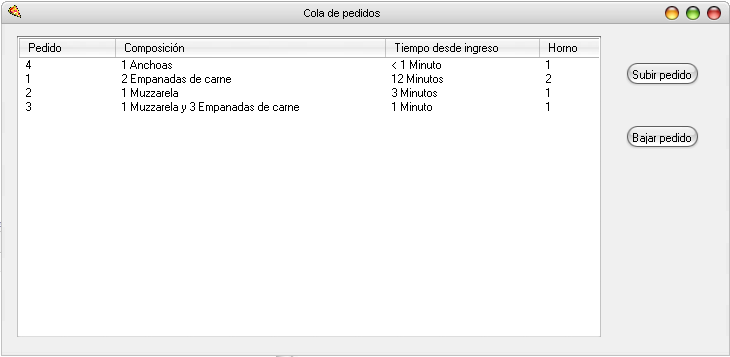
\includegraphics[scale=0.6]{./figuras/pantallaColaPedido3.png}
\caption{Prototipo de la vista de la cola de pedidos del encargado. El puede mover un pedido dandole mas o menos prioridad, en el ejemplo dio mas prioridad al pedido 4 recien ingresado}
\end{figure}

%operacion pedir proximo pedido a preparar
%TODO: aca hay que hacer diagramas seguro, pero no se me ocurren

\section{Cola de horno} 
La cola del horno es la cola que establece que pedido (que parte del mismo) se cocinara a continuaci�n. La cola se gestiona tambi�n de manera autom�tica. El maestro indica cuando saca algo de un pedido. El sistema informa que debe colocar al horno entonces. A partir del momento en que alguna parte del pedido es indicada para entrar al horno, el pedido pasa a ser considerado al horno. El sistema identifica que parte esta realmente en el horno, que parte aun no ingreso y que parte ya fue cocinada. Cuando todas las partes del pedido fueron cocinadas, se considera que el pedido fue cocinado. 

El sistema muestra que debe de colocarse en el horno. Cuando el maestro saca algo del horno, debe indicarselo al sistema a fin de que este pueda establecer que poner a continuaci�n.

La cola ingreso al horno admite varias politicas, una de ella es la de sectores agiles. En este caso, algunos modulos funcionan como modulos agiles y dan prioridad a los pedidos mas chicos. Es decir, que cuando se libera un modulo agil y el maestro pide que producto debe ingresar, el sistema tendra en cuenta la existencia de pedidos mas chicos que se puedan ingresar por completo al horno. 

El cambio de politica es ingresado por el encargado de pedidos, quien al cambiar la politica a sectores agiles, debe ingresar cuales son los modulos agiles. Las pol�ticas de horno no se modifican a lo largo del d�a (se elige al iniciar el sistema por la ma�ana). Adem�s, es global (no es por horno).

El tama�o y cantidad de los m�dulos del horno es configurable, sin embargo no se considera necesario un caso de uso para hacer esto. Lo mismo ocurre con la definici�n de pedido ``chico''.

A continuaci�n veremos en un diagrama de actividad las actividades que se producen cuando uno de los maestros indica que cocin� ciertos productos de un pedido. En el diagrama se nombra como pedido actual a aquel al cual pertenecen los productos que el maestro acaba de informar que termino de cocinar, ademas se considera que hay pedidos en la cola, de modo que el sistema debe informarle al maestro que poner a continuaci�n, esto no ocurre siempre, ya que si cuando el maestro informa que cocino algo no hay nada en la cola del horno, el sistema no le informa que poner sino hasta que exista algun pedido que deba ingresar al horno.


\begin{figure}[H]
\centering
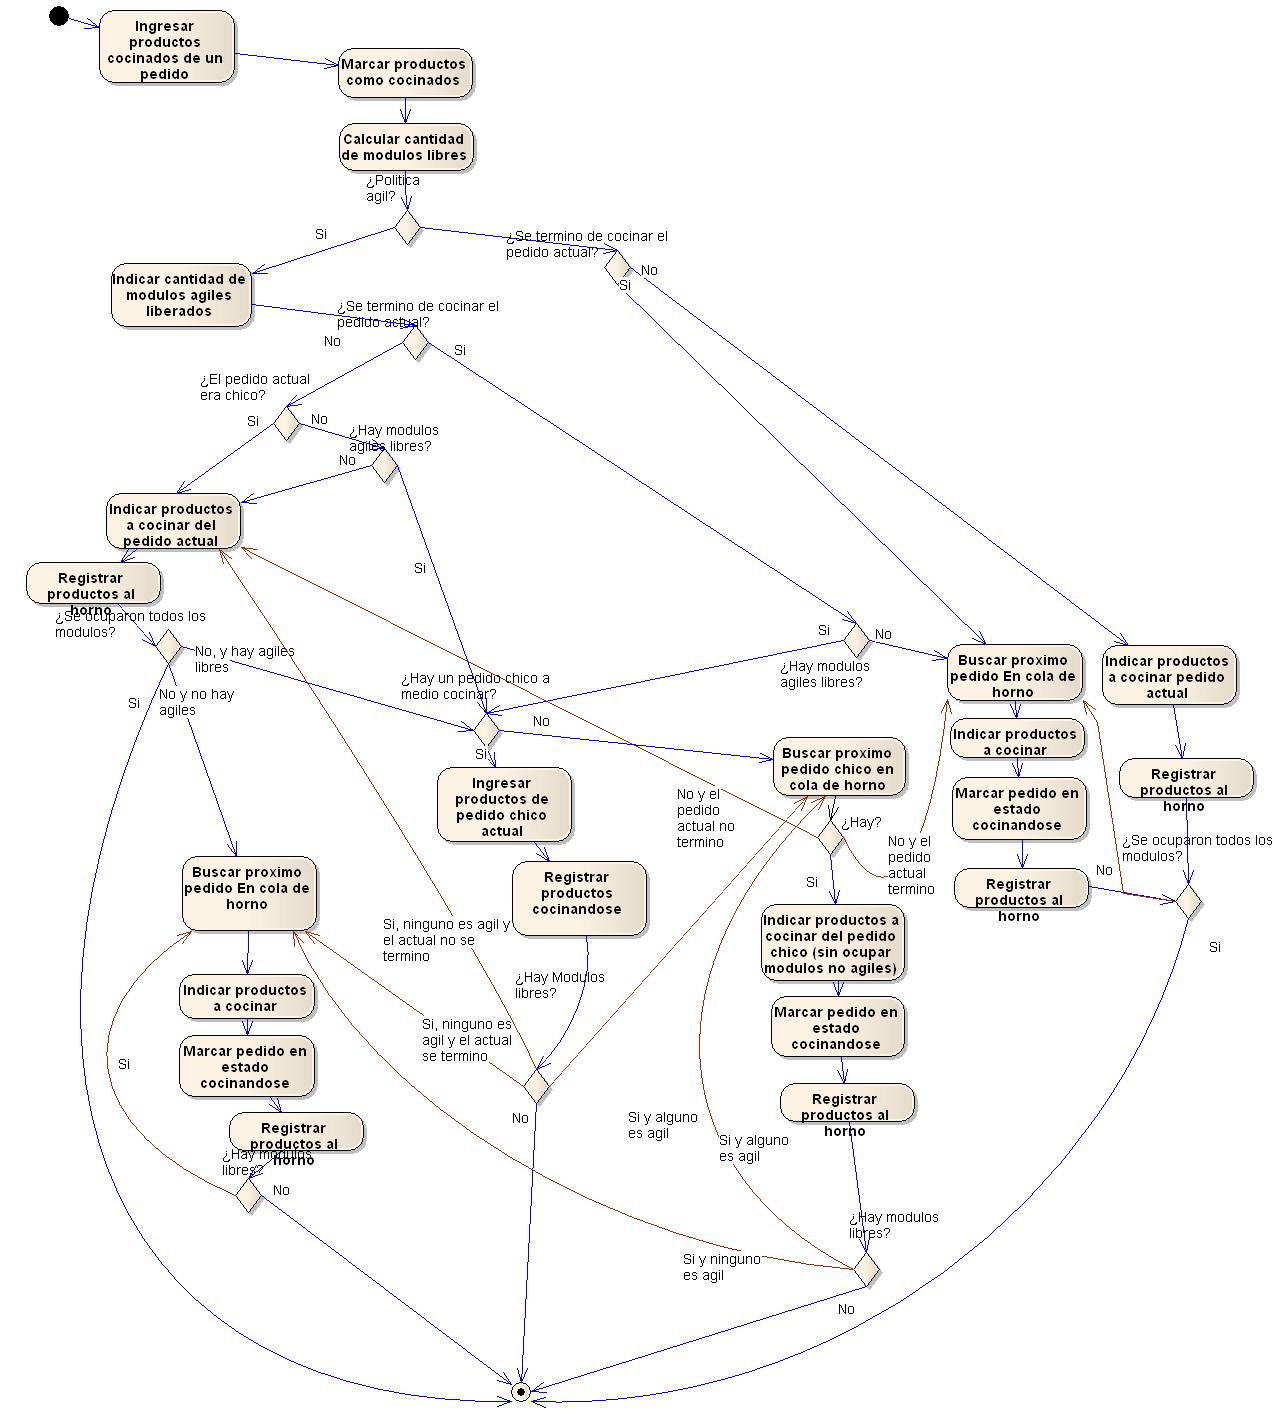
\includegraphics[scale=0.4]{figuras/actividadProxPedido.png}
\caption{Diagrama de actividad al informar productos cocinados}
\end{figure}

Lo que observamos es que en caso de politica agil el sistema debe ser informado de cuantos modulos agiles fueron liberados, esto podria evitarse si el sistema tuviera noci�n de que hay en cada modulo (ver posibilidades de mejora \ref{Extensiones}). Cuando se esta en politica agil lo que hace el sistema es buscar ocupar los modulos agiles, en la medida que se liberan, con pedidos chicos. En el caso de politica agil, puede ocurrir que existan dos pedidos con productos afuera del horno y dentro del horno. Por eso en el diagrama dice pedido actual y pedido chico actual. El pedido chico actual es un pedido chico que entro a cocinarse porque se libero algun modulo agil, pero quedo con alguno/s de sus productos sin cocinar

%Diagrama de actividad pedir proximo pedido

\section{Consulta de estado de pedidos}

Tanto el cliente como el encargado de pedidos pueden consultar el estado de un pedido determinado. El cliente puede hacerlo via web o mediante el encargado de pedidos por una llamada telefonica. Para consultar el estado de un pedido via web, el usuario tiene que autentificarse primero. Una vez autentificado podra acceder a la opci�n de consultar estado de sus pedidos. El sistema lista entonces los pedidos del usuario pendientes de entrega con su estado. 

Por otro lado, de manera similar el encargado de pedidos puede ingresar un n�mero de pedido para revisar su estado o ver los pedidos de un cliente.

%TODO: operacion del calculo de los tiempos

\section{Delivery}

El delivery posee una unica interacci�n con el sistema. Cuando entrega un pedido, debe enviar un mensaje SMS al sistema notificando la entrega del mismo.

Si el pedido no se pudo entregar el delivery debe notificarselo al encargado de pedidos, y el pedido pasara a ser considerado como cancelado

%todo: diagrama de actividad de entrega de pedidos


%\section{Alternativa de contingencia}
%El sistema posee la capacidad de funcionar en lo que denominamos modo de contingencia. Este modo esta pensado para premitir que el sistema siga siendo funcional aun cuando solo este disponible el puesto del encargado de pedidos.
  
%El sistema permite que toda la operatoria relacionada con la gesti�n y seguimiento de pedidos (recepci�n, asignaci�n de horno, armado, ingreso y salida de horno, despacho, control de entrega, actualizaci�n de lista de precios) se lleve adelante en el puesto del encargado de pedidos.

%En el modo de contingencia se considera que el software de facturaci�n no esta disponible, por lo cual la facturaci�n se realiza manualmente. Queda ademas fuera de este modo la consulta de estadisticas, asi como tambi�n la interacci�n directa del sistema con mozos, clientes y delivery.

%De esta manera el encargado de pedidos es el �nico agente que utiliza el sistema cuando se encuentra en este modo. Los clientes pueden hacer pedidos solo telefonicamente o en local a un mozo, mientras que los mozos deben comunicar el pedido al encargado para que este lo ingrese.

%De manera similar, los maestros deberan pedirle al encargado de pedidos que deben cocinar,preparar, asi como tambi�n informarle cuando terminaron de preparar algo o de cocinarlo.

%El delivery que en general utiliza SMS para informar al sistema la entrega de un pedido, ahora debera hacerlo comunicandose con el encargado de pedidos.

%Finalmente el due�o deber� informar al encargado de pedido los precios que pretende modificar.
\section{Alternativa de contingencia}
\label{alternativacontingencia}
\subsection{Diagrama de contexto del funcionamiento de contingencia}
%\begin{landscape}
%\begin{figure}[H]
%\centering
%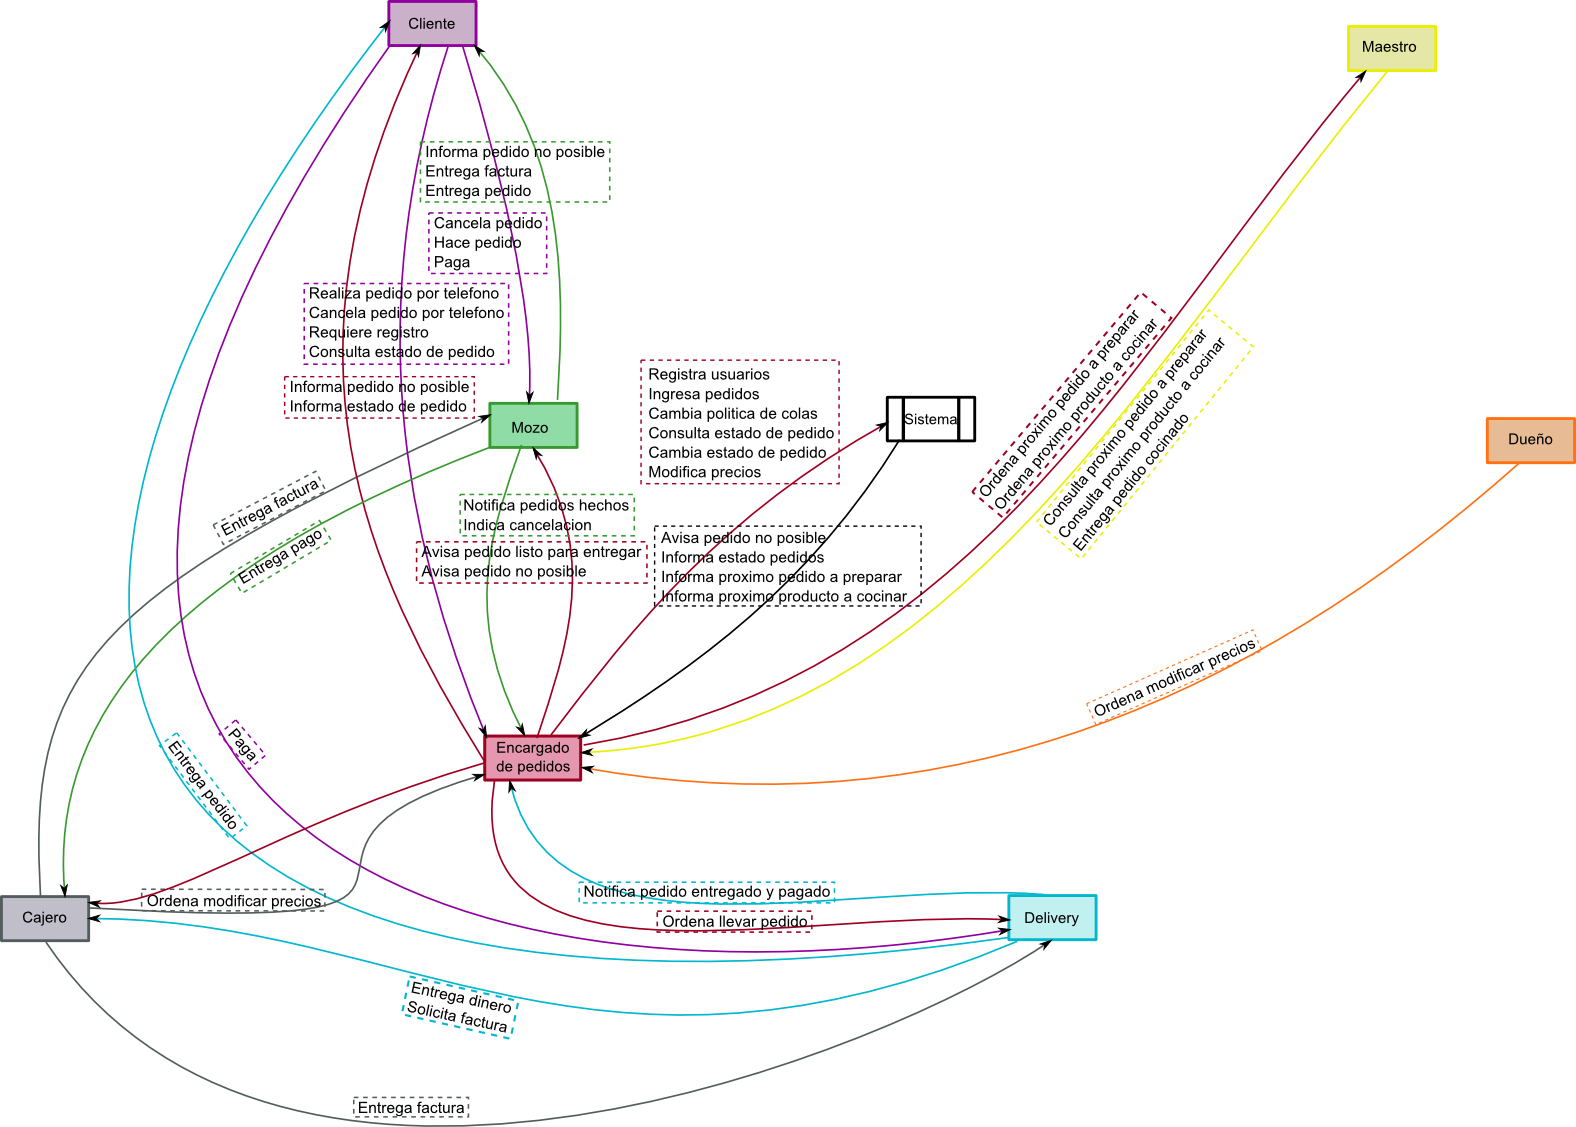
\includegraphics[height=17cm]{ContextoContingencia.png}
%\end{figure}
%\end{landscape}

Del diagrama observamos como las funciones principales en las que antes interactuaban otros agentes con el sistema, ahora son responsabilidad del encargado de pedidos, el cual suma a sus responsabilidades previas, tales como el ingreso de pedidos telefonicos, otras antes ajenas como informar pedidos preparados, etc.

Es muy importante notar la sobrecarga de trabajo del encargado de pedidos. La cantidad de tareas que debe desarrollar lo convierten en un cuello de botella para el funcionamiento de la pizzer�a, sin embargo dado que este escenario es para un caso de contingencia, en teoria un caso improbable, esta sobrecarga del encargado puede ser tolerada.

\subsection{Casos de uso contingencia}

A continuaci�n se presentan brevemente los casos de uso presentes cuando el sistema esta en estado de contingencia

\begin{figure}[H]
\centering
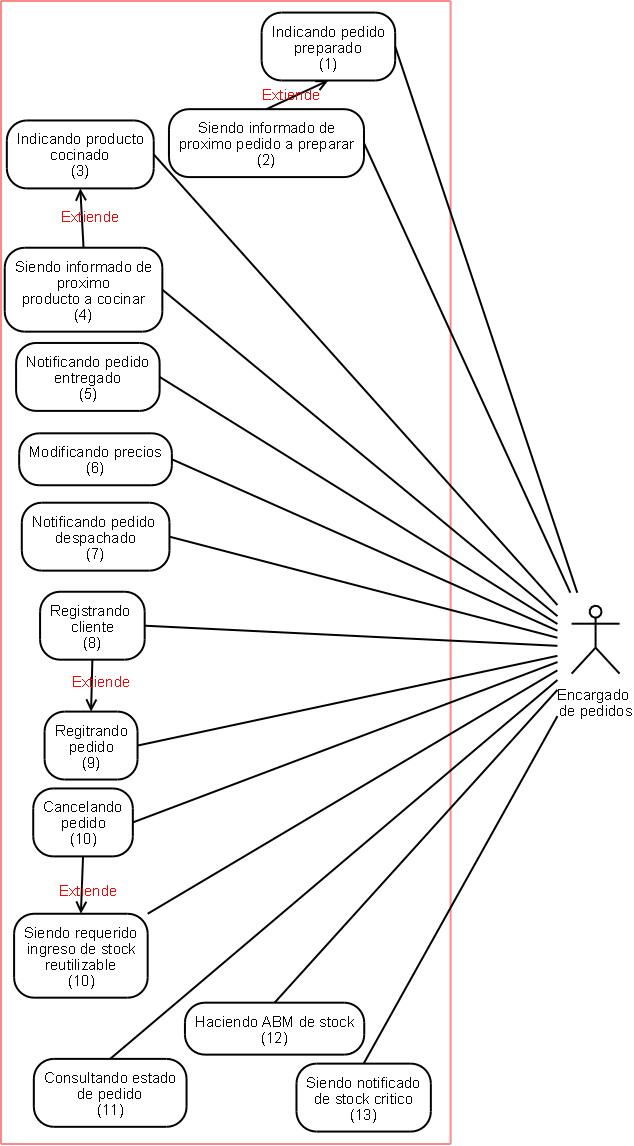
\includegraphics[height=16cm]{./figuras/casosDeUsoContingencia.png}
\end{figure}

El sistema posee la capacidad de funcionar en lo que denominamos modo de contingencia. Este modo esta pensado para permitir que siga siendo funcional a'un cuando solo est'e disponible el puesto del encargado de pedidos.
Podemos ver en el diagrama de contexto de contingencia el aumento de la densidad de eventos, con respecto al modo normal, que son controlados y monitoreados por el encargado de pedidos. Todas las responsabilidades que ten'ian los dem'as actores y que eran llevadas a cabo desde otras terminales del sistema ahora son tareas que los mismos deber'an llevar a cabo a trav'es del encargado de pedidos, ya que solo su terminal se mantiene en funcionamiento.

A continuaci'on describiremos brevemente los casos de uso en modo contingencia:
\begin{itemize}
\item Indicando pedido preparado y Indicando producto cocinado: el maestro le avisa al encargado de pedidos que termin'o la preparaci'on/cocci'on del pedido o producto y luego el encargado de pedidos procede a registrar tal evento en el sistema.
\item Siendo informado de proximo pedido a preparar y Siendo informado de proximo producto a cocinar: el encargado de pedidos solicita al sistema el proximo pedido/producto a preparar/cocinar y luego se lo informa al maestro.
\item Notificando pedido entregado: el delivery, al no poder enviar un mensaje al sistema para que registre la entrega (o cancelaci'on) del pedido, deber'a avisarle al encargado de pedidos para que este cambie el estado del mismo.
\item Modificando precios: el cajero o due�o desea cambiar el precio de los productos, para esto debe informarle al encargado de pedidos los datos necesarios para realizar la operaci'on. Este caso de uso reemplaza a Realizando ABM de productos, ya que hacer baja o alta de un producto no es una operacion cr'itica durante contingencia.
\item Notificando pedido despachado, Registrando cliente, Consultando estado de pedido y Cancelando pedido: estos casos de uso quedan igual a los casos en modo normal.
\item Registrando pedido: este caso de uso reemplaza a Registrando pedido telef'onico y Registrando pedido de mostrador. Su funcionamiento es igual a los anteriores.
\item Haciendo ABM de stock y Siendo notificado de stock cr'itico: ahora el encargado de pedidos asume las responsabilidades del encargado de stock. Estos son los mismos casos de uso que antes, aunque el actor es el encargado de pedidos.
\end{itemize}

Notese que la geeraci�n de archivo para facturaci'on en modo contingencia no est'a a cargo del sistema, por lo cual se realiza manualmente y est'a a cargo del cajero, como se puede ver en el diagrama de contexto de contingencia. Tambi'en queda fuera de este modo la consulta de estad'isticas, los pedidos por sms y, como ya fue dicho, el alta y baja de productos, ya que no son necesidades cr'iticas durante contingencia.

Los casos de uso de la alternativa de contingencia, son los que permiten satisfacer los requerimientos 16,17 y 18, ya que estos requerimientos eran los que establecian que el sistema deber�a ser capaz de funcionar con solo el puesto del encargado en estado funcional.

\section{Informacion estad�stica}
%FIXME: hay cosas q para calcularlas necesitamos info q no tenemos (segun el diag de concepto)
Con el fin de comprender m�s profundamente el comportamiento del negocio, desarrollamos para la pizzer�a un conjunto de indicadores que permitan analizar su rendimiento y predecir algunos de los par�metros que afectan su comportamiento, as� como optimizar algunas estrategias de venta y producci�n.

Los indicadores de rendimiento tienen por objetivo caracterizar el funcionamiento de la pizzer�a en un per�odo dado. Mediante el monitoreo del ingreso y salida de los pedidos, es posible realizar un seguimiento de algunos par�metros interesantes:
\begin{itemize}
\item \textbf{Tasa de producci�n de la cocina}: Permite evaluar el la capacidad de la cocina de atender pedidos, con el objeto de determinar sus posibilidades de producci�n y evaluar si en un momento dado la cocina funciona por debajo o por encima de su nivel habitual.
\item \textbf{Tasa de ingreso de pedidos}: Permite conocer la demanda que hubo en un momento dado y con esa informaci�n inferir la demanda de momentos futuros. Puede medirse de forma global o discriminada por origen de pedido, permitiendo observar cual es la forma m�s utilizada para ingresarlos.
\item \textbf{Tiempo medio de espera por un pedido}: Permite conocer el tiempo que debe esperar un cliente por su pedido en funci�n del momento en que realiz� su pedido. Puede medirse de forma discriminada para clientes locales o remotos.
\item \textbf{``Combos'' m�s populares}: Permite conocer algunos conjuntos de productos que suelen ser ordenados juntos por los clientes. 
\item \textbf{ ``Perfiles'' de cliente}: Permite evaluar los tipos de compras que realiza cada cliente gracias a la informaci�n personalizada que se tiene sobre cada uno. 
\item \textbf{Productos m�s populares}: Permite conocer cuales son los productos que circulan con mayor frecuencia y por tanto deber�an ser considerados m�s importantes para cuestiones tales como la ubicaci�n de los mismos en la carta.
\end{itemize}

En particular, el conocimiento sobre la demanda permite mantener un menor stock de productos, disminuyendo as� el costo financiero y manteniendo una mayor eficiencia en la administraci�n de los recursos. A su vez, determinar los productos y combinaciones m�s populares puede conducir a promociones m�s efectivas, as� como a disminuciones de costos por un mejor conocimiento de los insumos necesarios para su producci�n. Por �ltimo, los perfiles de cliente permiten ejecutar estrategias de fidelizaci�n: al conocer en detalle y de forma individual las compras que realiza cada cliente se puede determinar cuales son los clientes m�s importantes y en funci�n de eso ofrecerles alg�n tipo de beneficio.

\section{Modificaci�n de precios}
La modificaci�n de precios puede ser realizada por el due�o, o por el cajero. Para modificar precios se utiliza el sistema de ABM de productos que provee el sistema. (ver ABM de productos)

\section{ABM de productos}
El ABM de productos, permite ingresar nuevos productos, es decir nuevas variedades de pizzas, empanadas, etc. Al ingresar un nuevo producto se debe ingresar un tiempo estimado de cocci�n y preparaci�n. Por otro lado tambi�n se puede modificar los precios de los productos existentes, que no afectan a los pedidos ya registrados. Finalmente, tambi�n se puede dar de baja productos, por ejemplo productos que se venden muy poco.

%TODO: hacer operaciones abm

\section{ABM de stock}
El ABM de stock permite realizar altas, bajas y modificaciones de los kits y demas insumos para la elaboraci�n de productos. Ademas permite modificar el valor critico de cada insumo, de modo que el sistema pueda utilizar dicho valor para alertar al encargado de stock cuando la cantidad disponible de un producto descienda por debajo de dicho valor. La notificaci�n se realiza con un mensaje en pantalla 

Para ver como funciona el control por stock critico, analicemos las siguientes FSM, en las que se modela un ingreso de pedidos que consumen cierta cantidad de un stock determinado (figura \ref{ingresoDePedidos}) por simplicidad estamos usando que solo consume cierta cantidad de un insumo, pero se puede extender relativamente facil a varios insumos. El control de stock esta modelado en la FSM de la figura \ref{stockCritico}, como vemos, el sistema permite que se ingresen pedidos, pero cuando la cantidad de stock es menor al valor critico se produce un aviso, y luego se permite igualmente seguir ingresando pedidos. Cuando el encargado de stock \ref{encargadoStock} observa el aviso puede ingresar nuevos productos aumentando el stock. Entonces el sistema vuelve a monitorear el valor del stock para avisar si queda bajo el valor critico. En particula si el encargado deja el stock en un valor inferior al critico, el sistema volvera a mostrar el mensaje de stock critico.

En estas FSM utilizamos la variable, $stock : [0..MAX]$ que comienza inicializada en STOCK un valor constante. %TODO: ver q esta inicializacion aparezca en el diagrama
Por otro lado $critico$, $k$ y $n$ son valores constantes.

\begin{figure}[H]
\centering
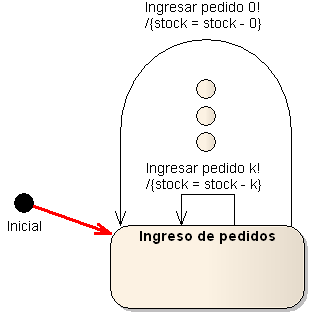
\includegraphics[scale=0.6]{./figuras/fsmingresador.png}
\caption{FSM ingresar pedidos}
\label{fsmIngresoPedidos}
\end{figure}

\begin{figure}[H]
\centering
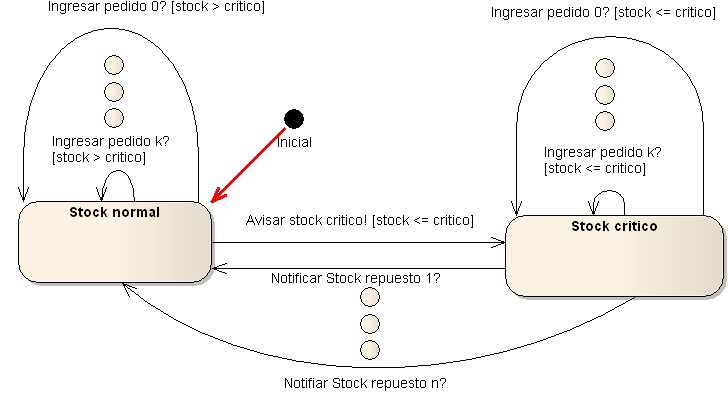
\includegraphics[scale=0.6]{./figuras/fsmstockcritico.png}
\caption{FSM aviso stock critico}
\label{fsmIngresoPedidos}
\end{figure}

\begin{figure}[H]
\centering
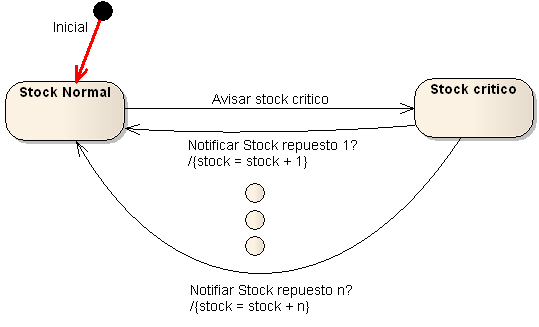
\includegraphics[scale=0.6]{./figuras/fsmreponerstock.png}
\caption{FSM responsable de stock}
\label{fsmIngresoPedidos}
\end{figure}
 
Entonces FSM Control de stock critico = FSM ingresar pedidos $||$ FSM aviso stock critico $||$ FSM responsable de stock

\section{Estimaci�n de tiempos}
A continuaci�n detallaremos las operaciones que permiten estimar el tiempo de finalizaci�n de un pedido. Notar que la misma es una estimaci�n, no intenta ser exacta, de hecho dado que no era requerido no se tiene en cuenta el tiempo de delivery, que en general podr�a no ser despreciable.

Para la estimaci�n utilizamos los tiempos de preparaci�n y de cocci�n aproximados dados por el maestro al momento que se ingresa un producto al sistema.

Veamos como es para el caso de un pedido recien ingresado, ya que para los otros casos es similar solo que no se cuenta el tiempo de las etapas que ya paso.

Primero se estima su tiempo de preparacion y coccion
 
Luego se estima el tiempo de preparacion y coccion de los productos que estan adelante de el en la cola de ingreso.

Luego se hace lo mismo para los pedidos que se estan preparando

Y finalmente se estima el tiempo de cocci�n de los pedidos que estan en la cola del horno correspondiente al pedido y de los que se estan cocinando.

Como vemos este valor dista de ser exacto, pero de hecho no pretende serlo, sino que sirve como una estimaci�n para el cliente.

Presentamos las operaciones a modo de quieries sin contexto que permiten estimar estos tiempos

Esta operacion nos permite obtener los pedidos que estan adelante del pedido p en la cola de preparacion

\textbf{pedidosAdelantePreparacion (p1:Pedido):set(pedido)\\}
Pedido.allInstances() \flecha  select (p $|$ p.estado = ingresado and p.posicionPreparaci�n \flecha  asOrderedSet() \flecha  first() $<$ p.posicionPreparaci�n \flecha asOrderedSet()\flecha first())

Esta calcula el tiempo de preparaci�n de un pedido en base a los tiempos de sus productos

\textbf{TiempoPreparacion(p:Pedido):Integer\\}
p.productos \flecha select(pr $|$ pr.iskindof(comida)) \flecha collect(pr $|$ pr.items() \flecha select(i $|$ i.pedidos = p)  \flecha asOrderedSet() \flecha first().cantidad * pr.asOclType(comida).tiempoPreparacion) \flecha sum()

Esta operacion permite calcular el tiempo de coccion de un pedido que tiene partes ya cocinadas

\textbf{TiempoDeCocci�nAlHorno(p:Pedido): Integer\\}
p.itemDe \flecha select(i $|$ i.producto.isKindOf(com)) \flecha collect(coccionDe \flecha  asOrderedSet() \flecha first()) \flecha collect(c $|$ c.itemDe.productos.\\ asOclType(Comida).tiempoCoccion * (c.itemDe.cantidad - c.cantidadCocinada)) \flecha sum() 

Esta nos permite obtener el tiempo de cocci�n de un pedido en base a los de sus productos

\textbf{TiempoDeCoccion(p:Pedido): Integer\\ }
p.productos \flecha select(pr $|$ pr.iskindof(comida)) \flecha collect(pr $|$ pr.items() \flecha select(i $|$ i.pedidos = p) \flecha asOrderedSet() \flecha first().cantidad * pr.asOclType(comida).tiempoCocion) \flecha sum()

Estas 3 operacinoes nos permiten conseguir a los pedidos que estan en preparacion, preparados (y esperan para el mismo horno que p tiene asignado) y por ultimo los pedidos que se estan cocinando en el horno asignado a p


\textbf{PedidosEnPreparacion() : Set(Pedido)\\}
Pedido.allInstances() \flecha select(p $|$ p.estado = En Preparacion)


\textbf{PedidosColaHorno(p:Pedido) : Set(Pedido)\\}
Pedido.allInstances() \flecha select(p1 $|$ p1.estado = Preparado and p.hornoDe = p1.hornoDe)


\textbf{PedidosHorno(p:pedido) : Set(Pedido)\\}
Pedido.allInstances() \flecha select(p1 $|$ p1.estado = Al horno and p.hornoDe = p1.hornoDe)

Estimamos entonces el tiempo hasta que p este listo

\textbf{EstimarTiempo(p: Pedido): Integer \\}
pedidosAdelantePreparacion \flecha collect(p1 $|$ TiempoDeCoccion(p1) + TiempoPrepracion(p1)) \flecha Sum() + pedidosEnPreparacion \flecha collect(p1 $|$ TiempoDeCoccion(p1) + TiempoPreparacion(p1)) \flecha Sum() + 
PedidosColaHorno(p) \flecha collect(p1 $|$ TiempoDeCoccion(p1)) +
PedidosHorno(p) \flecha collect(p1 $|$ TiempoDeCocionAlHorno(p1))
TiempoPreparacion(p) + TiempoCoccion(p)

\chapter{Ap�ndice I: Posibilidades de mejora}
\label{Extensiones}
%TODO: estimacion dinamica de tiempo de coccion de productos
%TODO: tal vez hacer algo de trazabilidad con esto?
Se detallan a continuaci�n algunas propuestas de mejora que consideramos pueden resultar de sumo inter�s para el funcionamiento de la pizzer�a. Estas mejoras se consideraron para su inclusi�n en el sistema especificado pero fueron dejadas de lado dadas las limitaciones de tiempo para el desarrollo.

La implementaci�n de estas funcionalidades podr� ser objeto de mejoras posteriores al sistema propuesto.

\section{Seguimiento de m�dulos del horno }

Una mejora sencilla de implementar es el seguimiento individual de cada m�dulo del horno as� como de qu� pedido lo ocupa en un momento dado. En la implementaci�n requerida, el sistema no puede determinar en qu� lugar del horno se encuentra un pedido.

Esto no representa una limitaci�n seria en contextos donde los tama�os y cualidades de los m�dulos son id�nticas en todos ellos. El seguimiento individual de cada m�dulo permitir�a tener divisiones irregulares del horno, lo cual puede ser necesario para algunos tipos de horno.

En cualquier caso, el seguimiento individual del m�dulo del horno permite ofrecer una mejora sustancial desde el punto de vista de usabilidad, ya que el individualizar cada m�dulo permite a un maestro indicar al sistema qu� pedido se ha terminado de cocinar sencillamente eligiendo cu�l es el m�dulo del horno que acaba de vaciar. Si los m�dulos son indistinguibles, el maestro deber� identificar el pedido dentro de una lista de pedidos en proceso de cocci�n, tarea que podr�a ser no trivial para pedidos similares.


\section{Seguimiento de tiempos por estado}

El hecho de seguir individualmente los tiempos que un pedido insume en cada estado ofrece una mejora importante desde un punto de vista estad�stico ya que permite individualizar los tiempos de cada parte del proceso de atenci�n de un pedido.

Si se dispone de esta informaci�n, se pueden hacer predicciones mucho m�s precisas del tiempo estimado para la salida de un pedido, o de la tasa de producci�n de la cocina, facilitando as� la indentificaci�n de cuellos de botella que limiten la capacidad de producci�n. 

La implementaci�n de esta funcionalidad se ve extendida por la caracter�stica de seguimiento individual de productos detallada m�s abajo


\section{Preparaci�n adelantada}

Al disponer de estad�sticas precisas sobre la demanda que recibe el local es posible, en funci�n de las predicciones hechas por el sistema, optimizar el uso de los recursos de producci�n del local abaratando as� costos.

Dado que el tama�o del staff de la pizzer�a depende principalmente de la cantidad de pedidos que se desea poder procesar en un lapso dado, es de esperarse que la pizzer�a emplee trabajadores suficientes para funcionar durante picos de demanda. Esto redunda en la disponibilidad de capacidad ociosa en los momentos de menor demanda. 

Si se pueden predecir adecuadamente los picos de demanda, el sistema puede indicar a los cocineros preparar pizzas que se sabe que se vender�n durante un pico de demanda. Al hacer esto durante momentos de capacidad ociosa, se puede maximizar la ocupaci�n de los cocineros manteniendo as� peque�o el tama�o del staff. 


Si se asume que el cuello de botella del proceso est� en los empleados, esto reduce los costos operativos del negocio, con lo  cual se trata de una caracter�stica muy deseable. Adem�s, el sistema puede controlar que los pedidos preparados no expiren sigui�ndolos individualmente.

% TODO: se puede hacer un grafico para ilustrar esto

\section{Carga diferida de pedidos}

El sistema contempla la necesidad de ser tolerante a fallos. Sin embargo, esta consideraci�n se limita a permitir la operaci�n de toda la pizzer�a a trav�s de la terminal del encargado de pedidos. Si bien esta funcionalidad es deseable, resulta importante tambi�n considerar qu� hacer en caso de una ca�da total. En la eventualidad de que esto ocurra, el sistema no podr� hacer ning�n procesamiento relativo al funcionamiento de la pizzer�a. 

Si bien no se puede hacer nada mientras la situaci�n que cause el problema se prolongue (falla de hardware, p�rdida de energ�a), tiene sentido permitir el ingreso diferido de pedidos que se procesaron manualmente durante la falla del sistema. La idea es registrar cuando el sistema vuelve a funcionar todos los eventos que se produjeron mientras �ste no era capaz de registrarlos.

Para esto es necesario agregar una interfaz especial del tipo ABM para el registro de dichos eventos. Esta interfaz deber�, adem�s de permitir ingresar los pedidos y sus datos, dejar que el usuario ingrese datos tales como los tiempos y duraciones de los eventos, y otras informaciones que durante la operatoria normal el sistema infiere por s� solo.

Esto permite realizar  un seguimiento apropiado del stock y ingresar datos sobre pedidos que de otro modo no ser�an registrados, con el fin de tener estad�sticas v�lidas del per�odo de falla.



\section{Seguimiento individual de cada producto}

Otra mejora interesante es ampliar el alcance del sistema de control de stock para permitir una visi�n m�s granular de los productos involucrados en el proceso de producci�n.

Esto abarca desde los lotes de stock hasta cada pizza producida, as� como eventualmente la relaci�n entre ambos (qu� lote de insumos fue utilizado para producir qu� pizza). Esto nos da algunas posibilidades interesantes, aunque produce un costo adicional importante de recursos ya que aumenta notoriamente la cantidad de datos que se almacenan.

Para empezar, es posible controlar los vencimientos de los insumos adquiridos adem�s de su stock, as� como la fecha de su compra y el costo de cada operaci�n. Esto permite no solo evitar problemas sanitarios, sino tambi�n observar la influencia de par�metros econ�micos como la inflaci�n en los costos de operaci�n de la pizzer�a.

En segunda instancia, controlar individualmente cada uno de los productos que salen del negocio permite mejorar sustancialmente la precisi�n de las estad�sticas y predicciones que puede hacer el sistema.

Por �ltimo, si se lleva registro de la vinculaci�n entre lotes de insumos y productos vendidos resulta m�s sencillo solucionar (o en su defecto, desvincularse de) responsabilidades en caso de tener alg�n problema sanitario. Si un cliente se enferma, el conocer exactamente cual es la partida de ingredientes que fueron utilizados en la preparaci�n de ese alimento permite aislarla para determinar si ten�a alg�n problema o sencillamente evitar seguirla utilizando.


\chapter{Glosario}
\section{Terminolog�a}
\begin{itemize}
\item \textbf{Pedido:} Se denomina ``pedido'' a todo pedido realizado por un cliente 
(a trav�s de alguno de los medios de contacto disponibles) y que ya ha sido 
procesado por el sistema. Un pedido no es tal, y no se registra informaci�n sobre �l,
hasta el momento en que se da de alta en el sistema.
\item \textbf{Encargado de pedidos:} El encargado de pedidos es un empleado cuya labor es la de administrar los pedidos y el funcionamiento generascontrola la facturaci�n y supervisa la distribuci�n de los pedidos. Adem�s tiene privilegios para situaciones especiales (reorganizaci�n de la cola de pedidos, cambios de pol�tica de pedidos, cancelaciones y acceso al ABM de usuarios). En caso de contingencia (sistema ca�do o con funcionalidad limitada), este agente deber� controlar el funcionamiento manual del sistema y posteriormente ingresar los datos de los pedidos recibidos para su registro en el sistema.
\item \textbf{Encargado de stock:} El encargado de stock es la persona responsable de
recibir las notificaciones relacionadas a los niveles de stock e ingresar los datos
respectivos a las altas y bajas del stock. En la mec�nica actual de la pizzer�a no
hay un encargado de stock definido. Si bien su papel ser� desempe�ado por alguno
de los otros agentes (due�o o encargado de pedidos), decidimos separar su rol puesto 
que se trata de una tarea independiente de las dem�s.
\item \textbf{Cajero:} El cajero se encarga de modificar los precios (capacidad que
comparte con el due�o), registrar los pagos que se hacen en el local, recibir el dinero
del \textit{delivery} e ingresar los pagos en el sistema, y solicitar la facturaci�n
de pedidos cuando sea necesario.
\item \textbf{Due�o:} El due�o es responsable de la gesti�n de la carta de la pizzer�a, sus precios y es el interesado en acceder a las estad�sticas sobre el funcionamiento del negocio.
\item \textbf{Cocinero:} El cocinero es cualquier persona que trabaja en la cocina. En principio es ya sea el maestro pizzero o el maestro empanadero, pero podr�a ser un ayudante de cocina en general.
\item \textbf{Estad�sticas:} Las estad�sticas son registros hist�ricos de los indicadores de rendimiento, que permiten evaluar la progresi�n del negocio a lo largo del tiempo.
\item \textbf{Indicadores de rendimiento:} Son valores num�ricos que describen el rendimiento de la pizzer�a en un per�odo determinado. Pueden depender de factores diversos. Algunos ejemplos de indicadores de rendimiento son la tasa de producci�n de la cocina, la tasa de ocupaci�n del horno, el tiempo medio de espera por un pedido o la cantidad de valoraciones negativas obtenidas por el sistema de feedback. Algunos de ellos se le presentan al encargado de pedidos en tiempo real.
\item \textbf{Maestro Pizzero:} Es el cocinero encargado de las pizzas, que se ocupa de determinar los ingredientes que componen a una pizza dada, prepararla y supervisar su cocci�n si se hace en su horno. En el contexto del sistema, es responsable de los cambios de estado de los pedidos en la secci�n que concierne a la cocina.
\item \textbf{Maestro Empanadero:} An�logo al maestro pizzero pero para la preparaci�n de empanadas.
\item \textbf{Mesero o Mozo:} Es el responsable de atender a los clientes en las mesas y registrar sus pedidos en el PDA que luego los transfiere al sistema. Si el sistema est� degradado y no dispone del PDA, registrar los pedidos mentalmente o en papel y luego se los entrega al encargado de pedidos.
\item \textbf{Cliente:} Es cualquier individuo que est� interesado en adquirir productos de la pizzer�a, a trav�s de cualquiera de los medios de contacto y pedido.
\item \textbf{Cliente local:} Cliente que concurre personalmente al local y es atendido por un mesero en su mesas.
\item \textbf{Cliente remoto:} Cliente que hace su pedido desde su casa u otro lugar y requiere que le sea entregado por el servicio de delivery.
\item \textbf{Cliente telef�nico:} Cliente remoto que realiza su pedido por tel�fono (es atendido por el encargado de pedidos que a su vez ingresa el pedido en el sistema manualmente.
\item \textbf{Cliente Web:} Cliente remoto que realiza su pedido a trav�s de la p�gina web de la pizzer�a. El sistema registra su pedido sin ninguna intervenci�n humana.
\item \textbf{Cliente SMS:} Cliente remoto que realiza su pedido a trav�s de mensajes de texto. El sistema registra su pedido sin ninguna intervenci�n humana.
\item \textbf{Servicio de delivery:} Servicio de entrega a domicilio de los pedidos. Este servicio se subcontrata a un tercero que provee toda la log�stica de entregas, debiendo la pizzer�a �nicamente indicar las entregas que deben realizarse.
\item \textbf{Cola de pedidos:} La cola de pedidos almacena los pedidos que deben prepararse y entregarse, y permite priorizarlos seg�n la pol�tica de cola elegida. Dichar priorizaci�n puede ser manual o autom�tica. 
\item \textbf{Pol�tica de cola:} La pol�tica de cola es el criterio que se utiliza para determinar la ubicaci�n de los pedidos en la cola de pedidos. En general se utiliza este t�rmino para denominar a un criterio algor�timico automatizado de ordenamiento de los pedidos, pero la pol�tica puede ser algo tan simple como ``el encargado de pedidos ordena la cola de pedidos''.
\item \textbf{Sistema de facturaci�n:} Es un sistema inform�tico externo que mediante una interfaz predefinida se encarga de la facturaci�n y emisi�n de comprobantes de todas las ventas que se producen en la pizzer�a.
\item \textbf{Sistema de SMS:} Es un sistema inform�tico externo que provee un servicio de interfaz con las empresas de telefon�a celular, permitiendo que el sistema procese mensajes que los clientes env�an a trav�s de SMS.
\item \textbf{Pedido diferido:} Los pedidos diferidos son pedidos que se realizaron por fuera del sistema (por diversas razones, una de las cuales puede ser una ca�da del sistema). Se permite al encargado registrar dichos pedidos despu�s de que fueron procesados manualmente para que sean tenidos en cuenta en las estad�sticas.
\item \textbf{Productos preparados de antemano:} En alguna situaciones pueden prepararse los productos de antemano dej�ndolos listos para ingresar al horno, antes de que los pedidos sean efectuados. Esto permite preparar la cocina para un pico de demanda. Es importante no confundir con las materias primas necesarias para la preparaci�n.
\end{itemize}

\section{Estados de pedido}
Los estados en los que puede encontrarse un pedido una vez que ingres� al sistema son:
\begin{itemize}
\item Ingresado: El pedido pas� los chequeos necesarios, se determin� que es posible llevarlo a cabo con �xito y se ingres� al sistema, yendo a parar a una cola donde espera a que la cocina est� lista para prepararlo.
\item	En preparaci�n: El pedido ya fue recibido por la cocina y est� siendo preparado por un cocinero.
\item	Preparado: El pedido ya fue preparado en su totalidad y est� listo para ingresar al horno cuando haya lugar disponible.
\item	En el horno: El pedido (o al menos una de sus partes) est� en el horno.
\item	Listo: El pedido est� listo para ser entregado al cliente.
\item	Enviado: El pedido fue entregado al delivery para su entrega a domicilio.
\item	Finalizado: El pedido fue entregado con �xito (ya sea a la mesa o a domicilio).
\item	Cancelado: El pedido fue cancelado antes de su entrega.
\end{itemize}
\begin{figure}
\centering
\includegraphics[scale=0.25]{ciclo_pedido.png}
\end{figure}

En breve, un proceso ingresa al sistema cuando es requerido por un cliente por alg�n medio de comunicaci�n. Enseguida se indica a la cocina que el pedido debe ser preparado. Una vez completada la preparaci�n de la comida, los responsables de cocina lo indican al sistema que planifica de forma independiente la asignaci�n de lugares en los hornos. Finalmente, despu�s de que el pedido es horneado, se entrega a la mesa o al delivery seg�n corresponda. Por �ltimo cuando existe confirmaci�n de la entrega se marca el pedido como finalizado y se almacena con fines de registro. El pedido puede ser cancelado en cualquier punto (salvo despu�s de ser finalizado), con implicaciones varias en el sistema de control de stock.

Los estados presentados tienen utilidad para el sistema puesto que hay necesidad de indicar al cliente sobre el estado de su pedido. As�, se podr� indicar si un pedido est� siendo preparado o ya fue enviado al destinatario. Si bien para estos fines alcanza con 3 estados (preparando, enviando, finalizado), se agregan los dem�s con fines de control para el sistema. Adem�s, la granularidad m�s fina permite al sistema hacer predicciones y organizaciones m�s eficientes del uso de los recursos. Por ejemplo, al controlar los tiempos de preparaci�n por separado de los de horneado resulta m�s sencillo, en caso de un cuello de botella en la cocina, determinar cual es el factor limitante.

\label{LastPage}
\end{document}
